\title{Compensating a Power Amplifier using Iterative Learning Control : from Design to Realisation  }
\author{Jules Hammenecker \\ Brussels Faculty of Engineering \\ Vrije Universiteit Brussel - Universit\'e Libre de Bruxelles}
\date{2014-2015}

\documentclass[a4paper,openright,twoside]{report}
	
	%%% FONTS %%%%
	\usepackage{times}
	\usepackage{a4wide}
	%%% FIGURES %%%
	\usepackage[pdftex]{graphicx}
	\usepackage{caption,subcaption}
	\usepackage{hyperref}
	\usepackage{pgfplots,tikz}
	\pgfplotsset{compat=newest}
	\pgfplotsset{plot coordinates/math parser=false}
		\newlength\figureheight 
		\newlength\figurewidth 
	\usetikzlibrary{external}
	\tikzexternalize[prefix=tikz/]

	%%% MATHS %%%
	\usepackage[cmex10]{amsmath}
	\usepackage{amsthm}
	\usepackage{steinmetz}
		\newtheorem{definition}{Definition}
	%%% PDF %%%
	\usepackage{hyperref}
\begin{document}

\maketitle

\section*{Thank You Note}

\begin{abstract}
	
\end{abstract}

\tableofcontents

\chapter{Introduction} 											
	\section{Why Digital Predistortion?}
	
	Power amplifiers are used in almost all wireless communication devices. They amplify the communication signal such that a good signal to noise ratio is obtained. They also are an important power consuming block in a communication chain. A power amplifier is often operated in a nonlinear operation mode to improve its efficiency. This nonlinear behavior should be compensated in a later step to reach the strict telecommunication requirements.
	A Digital Pre-Distortion (DPD) is a common technique to linearize the input-output behavior of a power amplifier. With DPD the input signal of the amplifier is modified such that the desired (i.e. linear) behavior is obtained. 

\section{Current Techniques of DPD}
	\subsection{Direct and Indirect Learning}
	\subsection{Nonlinear Models}
\section{The Best Linear Approximation}
	\subsection{What is the BLA?}
	\subsection{How to measure it?}
	\subsection{Out of Band BLA and the Tickler Tone}

\section{Iterative Learning Control}
	\subsection{The Algorithm}
	\subsection{Properties}
\chapter{Using the BLA in ILC for DPD} 							
	%
% Chapter : Using the BLA in ILC for DPD
%
\section{Introduction}

The plethora of abbreviations used in this title only hides a simple concept. What if one uses the BLA in the system inversion algorithm in ILC?

\section{The Blocky Tought Experiment}

		A nonlinear dynamic system can alternatively be represented by the combination of a linear transfer function $G_{BLA}$ and a nonlinear function F.
		\begin{figure}[hbtp]
			\centering
			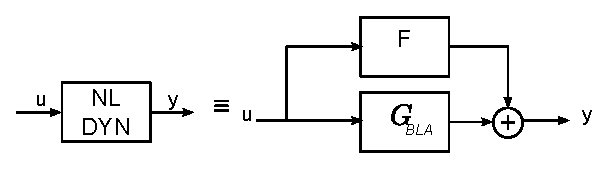
\includegraphics[scale=0.7]{images/lego1}
			\caption{Alternative representations of a nonlinear system. }
		\end{figure}
	
		\begin{figure}[hbtp]
			\centering
			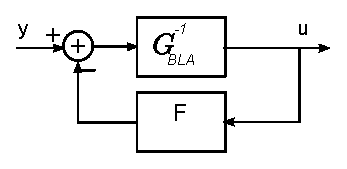
\includegraphics[scale=0.7]{images/lego2}
			\caption{Switching the input and output, creating the inverse of the nonlinear system. }
		\end{figure}

		\begin{figure}[hbtp]
			\centering
			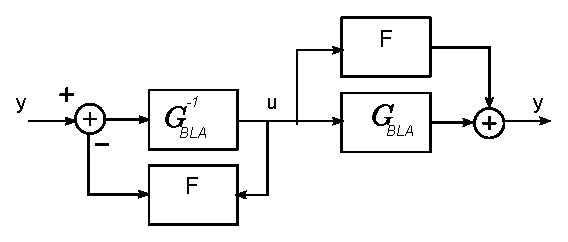
\includegraphics[scale=0.7]{images/lego3}
			\caption{Connecting the inverse and the original system together. }
		\end{figure}

		\begin{figure}[hbtp]
			\centering
			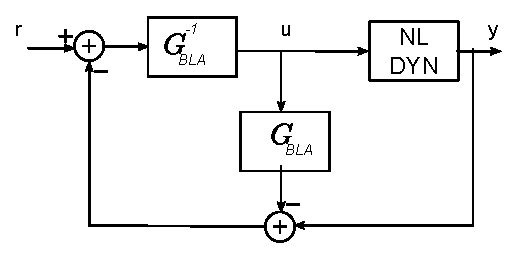
\includegraphics[scale=0.7]{images/lego4}
			\caption{Getting creative with the blocks. }
		\end{figure}

		\begin{figure}[hbtp]
			\centering
			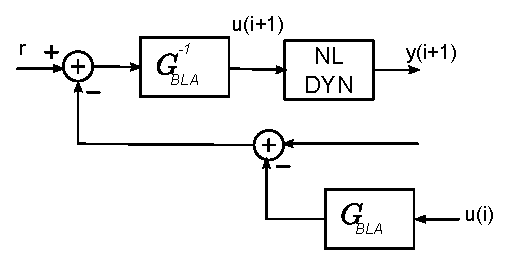
\includegraphics[scale=0.7]{images/lego5}
			\caption{Cut the loop! }
		\end{figure}

		\begin{figure}[hbtp]
			\centering
			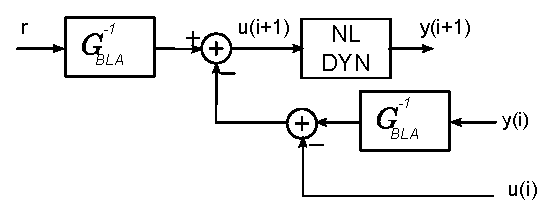
\includegraphics[scale=0.7]{images/lego6}
			\caption{Reorganise the blocks one last time. }
		\end{figure}

\section{Why can it work?}
\section{Creation of a standalone DPD}
\section{Estimating the Preinverse}
\chapter{Simulation Results} 									
	%
% Chapter : Simulations
%
\section{ILC with BLA}

	\subsection{Proof of Concept}
	Before constructing a solid framework for predistortion using ILC, a small number of simulations on test systems will be run to estimate the performance of this technique. A description of the systems will be given, followed by the measurement of their BLAs. The ILC compensation algorithm.

	\subsubsection{Presentation of Test Systems}
	\begin{description}
			\item[The Static Nonlinearity] that obeys the function \verb+y = 10*tanh(x/5)+

			 \item[The Wiener System] is a linear dynamic system followed by a static nonlinearity. The linear block is a Chebyshev filter and the nonlinearity is a $tanh()$ function. The MATLAB parameters of this system are as follows:
			\begin{enumerate}
			 	\item Input Block  : \verb+cheby1(1,1,2*1/15)+
			 	\item Nonlinearity : \verb+5*tanh(x/5)+
			 \end{enumerate} 

			\item[The Wiener Hammerstein System] which is a static nonlinearity sandwiched between two linear dynamic blocks. This particular system consists of two discrete-time Chebyshev filters and a $tanh()$ function as nonlinearity.
			The MATLAB parameters of this system are as follows:
			\begin{enumerate}
			 	\item Input Block  : \verb+cheby1(1,1,2*1/15)+
			 	\item Nonlinearity : \verb+5*tanh(x/1.2)+
			 	\item Output Block : \verb+cheby1(3,1,2*1/20)+
			 \end{enumerate} 
			 Additionally, measurement noise is simulated only on this system by adding zero-mean gaussian noise with $\sigma= 3.10^{-3}$
	\end{description}

	\subsubsection{Measuring the Best Linear Approximation}
	In figure \ref{fig:sim_BLA}, the BLA of each test system is plotted. All measurements had the same parameters that can be found in table 25 independent realisations, 2 measurement periods, 1 transient period and input signal rms of $0.3$.

	\begin{table}
	\renewcommand{\arraystretch}{1.3} \centering \caption{Parameters of multisine for robust measurement.} \label{robustparam} 
	\begin{tabular}
		{|c|c|} \hline Realizations M & 10\\
		\hline Periods P & 2\\
		\hline Excited Bandwith  & 0 to 0.1 $\frac{cycles}{sample}$  \\
		\hline Number of samples N & 4096\\
		\hline Multisine rms & 0.3 \\
		\hline 
	\end{tabular}
	\end{table}

	\begin{figure}
        \centering
        \begin{subfigure}[b]{0.3\textwidth}
            \centering
            \setlength\figureheight{3cm} 
			\setlength\figurewidth{0.5\linewidth}
			% This file was created by matlab2tikz.
% Minimal pgfplots version: 1.3
%
%The latest updates can be retrieved from
%  http://www.mathworks.com/matlabcentral/fileexchange/22022-matlab2tikz
%where you can also make suggestions and rate matlab2tikz.
%
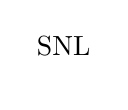
\begin{tikzpicture}

\begin{axis}[%
width=0.956388\figurewidth,
height=\figureheight,
at={(0\figurewidth,0\figureheight)},
scale only axis,
every outer x axis line/.append style={black},
every x tick label/.append style={font=\color{black}},
xtick={0,0.1},
xmin=0,
xmax=0.1,
xlabel={Frequency f/fs},
every outer y axis line/.append style={black},
every y tick label/.append style={font=\color{black}},
ymin=-70,
ymax=10,
ylabel={Amplitude [dB]},
title={SNL},
axis x line*=bottom,
axis y line*=left
]
\addplot [color=black,solid,forget plot]
  table[row sep=crcr]{%
0.000244140625	5.99642524383802\\
0.00048828125	5.9902268734636\\
0.000732421875	6.00033420698668\\
0.0009765625	5.98775583874669\\
0.001220703125	5.9937756549262\\
0.00146484375	5.98309266547375\\
0.001708984375	5.99249999271331\\
0.001953125	5.98792642903419\\
0.002197265625	5.98941336841125\\
0.00244140625	5.98903959592496\\
0.002685546875	5.99252567889374\\
0.0029296875	5.99531752664865\\
0.003173828125	5.98724152316174\\
0.00341796875	5.98835707875429\\
0.003662109375	5.9844551700528\\
0.00390625	5.99409356864373\\
0.004150390625	5.98924665633172\\
0.00439453125	6.00122404659692\\
0.004638671875	5.98972374544599\\
0.0048828125	5.99853959518913\\
0.005126953125	5.98747038362569\\
0.00537109375	5.98920027045995\\
0.005615234375	5.98676252216791\\
0.005859375	5.99036405586514\\
0.006103515625	5.9780661615041\\
0.00634765625	5.99276035694476\\
0.006591796875	5.98840101029219\\
0.0068359375	5.99367369692294\\
0.007080078125	5.99189201157185\\
0.00732421875	5.98455454366717\\
0.007568359375	5.98972372162035\\
0.0078125	5.99412306186849\\
0.008056640625	5.99400462825167\\
0.00830078125	5.99389158834833\\
0.008544921875	5.99356740491532\\
0.0087890625	5.99195395376199\\
0.009033203125	5.98718483226742\\
0.00927734375	5.98721432525628\\
0.009521484375	5.98296363108108\\
0.009765625	5.98408613685064\\
0.010009765625	5.9894135552463\\
0.01025390625	5.99283208940545\\
0.010498046875	5.99088621035764\\
0.0107421875	5.98217792723312\\
0.010986328125	5.99337540269931\\
0.01123046875	5.98949539097896\\
0.011474609375	5.99107110360586\\
0.01171875	5.98916380235607\\
0.011962890625	5.99244401028875\\
0.01220703125	5.98897681306181\\
0.012451171875	5.99145378183937\\
0.0126953125	5.98501701407361\\
0.012939453125	5.99270444013945\\
0.01318359375	5.98703023950935\\
0.013427734375	5.97976844920072\\
0.013671875	5.98601026896\\
0.013916015625	5.98814253274304\\
0.01416015625	5.98653234827793\\
0.014404296875	5.99583244021426\\
0.0146484375	5.98139759754741\\
0.014892578125	5.9855128165425\\
0.01513671875	5.98805006047951\\
0.015380859375	5.98849919476595\\
0.015625	5.98302268913915\\
0.015869140625	5.99022236304751\\
0.01611328125	5.99059547066025\\
0.016357421875	5.99395392582511\\
0.0166015625	5.98968960683942\\
0.016845703125	5.99392455553186\\
0.01708984375	5.99941861355518\\
0.017333984375	5.99713778362155\\
0.017578125	5.98856523288759\\
0.017822265625	6.00448938031957\\
0.01806640625	5.99566788313501\\
0.018310546875	5.98345218157436\\
0.0185546875	5.99051560164287\\
0.018798828125	5.98819756886786\\
0.01904296875	5.99582079874642\\
0.019287109375	5.98182166887182\\
0.01953125	5.98885966065313\\
0.019775390625	5.99185508350672\\
0.02001953125	5.98893340494283\\
0.020263671875	5.98718017040363\\
0.0205078125	5.99409259760972\\
0.020751953125	5.99471694807886\\
0.02099609375	5.99210452046117\\
0.021240234375	5.98692743072149\\
0.021484375	5.98891827840043\\
0.021728515625	5.98678813275041\\
0.02197265625	5.99044535125705\\
0.022216796875	5.99046881976756\\
0.0224609375	5.98970673152769\\
0.022705078125	5.98430278934762\\
0.02294921875	5.98445517525317\\
0.023193359375	5.99270895706439\\
0.0234375	5.99146214745588\\
0.023681640625	5.98741937389843\\
0.02392578125	5.98964928964\\
0.024169921875	5.98548961623976\\
0.0244140625	5.99094643692621\\
0.024658203125	5.99278470517027\\
0.02490234375	5.98524581115663\\
0.025146484375	5.99365173233548\\
0.025390625	5.99450853250914\\
0.025634765625	5.98555499897236\\
0.02587890625	5.99050923431082\\
0.026123046875	5.98385074726974\\
0.0263671875	5.99283765188119\\
0.026611328125	5.98553810556569\\
0.02685546875	5.98924281232166\\
0.027099609375	5.98448900598089\\
0.02734375	5.987207808981\\
0.027587890625	6.00062954171938\\
0.02783203125	5.99348597552898\\
0.028076171875	5.98055694451034\\
0.0283203125	5.98785658254735\\
0.028564453125	5.99120719718383\\
0.02880859375	5.99077943207465\\
0.029052734375	5.98508677381341\\
0.029296875	5.98631195072028\\
0.029541015625	5.98562974585428\\
0.02978515625	5.98953063711451\\
0.030029296875	5.98762201594911\\
0.0302734375	5.99336884113029\\
0.030517578125	5.99357186921958\\
0.03076171875	5.99222474404377\\
0.031005859375	5.98897132807838\\
0.03125	5.98788061671905\\
0.031494140625	5.99786067378471\\
0.03173828125	5.99642971306361\\
0.031982421875	5.98160204201491\\
0.0322265625	5.98599811347981\\
0.032470703125	5.99784882912536\\
0.03271484375	5.9905299612002\\
0.032958984375	5.99214781735282\\
0.033203125	5.99263662830708\\
0.033447265625	5.99339438340087\\
0.03369140625	5.98698337690291\\
0.033935546875	5.99629826349104\\
0.0341796875	6.00335306458783\\
0.034423828125	5.99358223683595\\
0.03466796875	5.99342437230638\\
0.034912109375	5.98496343059526\\
0.03515625	6.0017625827814\\
0.035400390625	5.99053310989359\\
0.03564453125	5.99291949941295\\
0.035888671875	5.99778781185717\\
0.0361328125	5.99208968814503\\
0.036376953125	5.99667804394835\\
0.03662109375	5.98718983449055\\
0.036865234375	5.99696668000416\\
0.037109375	5.99281303263251\\
0.037353515625	5.98499244430138\\
0.03759765625	5.9879607102792\\
0.037841796875	5.9883207973773\\
0.0380859375	5.99107863688022\\
0.038330078125	5.98915827068765\\
0.03857421875	5.99700293608458\\
0.038818359375	5.99446039452431\\
0.0390625	5.99012801943576\\
0.039306640625	5.98257768072693\\
0.03955078125	5.99166840256447\\
0.039794921875	5.98847394898053\\
0.0400390625	5.98735646930203\\
0.040283203125	5.98999002470413\\
0.04052734375	5.99055235785085\\
0.040771484375	5.99181127477578\\
0.041015625	5.99107121534485\\
0.041259765625	5.98434939356184\\
0.04150390625	5.98457213461825\\
0.041748046875	5.98927115676355\\
0.0419921875	5.99173107128598\\
0.042236328125	5.98513949129284\\
0.04248046875	5.9902529813296\\
0.042724609375	5.99270630923598\\
0.04296875	5.99168735975678\\
0.043212890625	5.9820090114618\\
0.04345703125	5.98830429898703\\
0.043701171875	5.99668284607355\\
0.0439453125	5.98984208969028\\
0.044189453125	5.98936307144947\\
0.04443359375	5.994281901688\\
0.044677734375	5.98531533281948\\
0.044921875	5.98456554465577\\
0.045166015625	5.9909428651826\\
0.04541015625	5.99545019231249\\
0.045654296875	5.99975590957382\\
0.0458984375	5.99537733504422\\
0.046142578125	5.9910358550498\\
0.04638671875	5.9924896118157\\
0.046630859375	5.9861407542196\\
0.046875	5.98856589720259\\
0.047119140625	5.98887996489481\\
0.04736328125	5.98882191751534\\
0.047607421875	5.99706934139419\\
0.0478515625	5.99346889327552\\
0.048095703125	5.98947494509963\\
0.04833984375	5.99128536428913\\
0.048583984375	5.98936832016017\\
0.048828125	5.98399501940474\\
0.049072265625	5.98697934665751\\
0.04931640625	5.99406995176435\\
0.049560546875	5.99636789510879\\
0.0498046875	5.99416726537254\\
0.050048828125	5.99210114782056\\
0.05029296875	5.99270377604853\\
0.050537109375	5.99410107803965\\
0.05078125	5.98538818562849\\
0.051025390625	5.99417640026167\\
0.05126953125	5.98116755821115\\
0.051513671875	5.99208269181099\\
0.0517578125	5.99238577164675\\
0.052001953125	5.99768711968949\\
0.05224609375	5.98695162700551\\
0.052490234375	5.98977639075969\\
0.052734375	5.9898827694218\\
0.052978515625	5.99313897371189\\
0.05322265625	5.99329820602702\\
0.053466796875	5.9889119272994\\
0.0537109375	5.99406665710501\\
0.053955078125	5.99569084991191\\
0.05419921875	5.98689636056815\\
0.054443359375	5.9877584690596\\
0.0546875	5.99013443449047\\
0.054931640625	5.97625293365843\\
0.05517578125	5.9907243758293\\
0.055419921875	5.99161354158736\\
0.0556640625	5.98577005409794\\
0.055908203125	5.98952807556469\\
0.05615234375	5.99343318934939\\
0.056396484375	5.98924910290407\\
0.056640625	5.98424838726532\\
0.056884765625	5.99528665817206\\
0.05712890625	5.99280025476457\\
0.057373046875	5.99037935491475\\
0.0576171875	5.99091020989329\\
0.057861328125	5.97962254665055\\
0.05810546875	5.99234790520302\\
0.058349609375	5.98712119926341\\
0.05859375	5.99356088312811\\
0.058837890625	5.99097408717194\\
0.05908203125	5.99411822947832\\
0.059326171875	5.99801268927314\\
0.0595703125	5.9908540505732\\
0.059814453125	5.9909416856799\\
0.06005859375	5.98925340019048\\
0.060302734375	5.98878457998364\\
0.060546875	6.001247575381\\
0.060791015625	5.98918733698241\\
0.06103515625	5.98580537801024\\
0.061279296875	5.98696395860082\\
0.0615234375	5.98552777940137\\
0.061767578125	5.9975267437901\\
0.06201171875	5.99416222988845\\
0.062255859375	5.99246600364847\\
0.0625	5.99094430715672\\
0.062744140625	5.99190838249672\\
0.06298828125	5.98770845254359\\
0.063232421875	5.9805402380041\\
0.0634765625	5.98897184176042\\
0.063720703125	5.99067374588657\\
0.06396484375	5.99905493186179\\
0.064208984375	5.99050377787438\\
0.064453125	5.99120823251172\\
0.064697265625	5.99374488753386\\
0.06494140625	5.99334555970074\\
0.065185546875	5.99133206060162\\
0.0654296875	5.98197888011811\\
0.065673828125	5.99044234060761\\
0.06591796875	5.99017111179938\\
0.066162109375	5.99338407267044\\
0.06640625	5.99685295931738\\
0.066650390625	5.98727903623399\\
0.06689453125	5.9901942301633\\
0.067138671875	5.99054457371005\\
0.0673828125	5.9881775255871\\
0.067626953125	5.99500875246207\\
0.06787109375	5.99503819017684\\
0.068115234375	5.99089541426463\\
0.068359375	5.98967676246787\\
0.068603515625	5.98941754184943\\
0.06884765625	5.99199817100856\\
0.069091796875	5.98555667142574\\
0.0693359375	5.98731030213207\\
0.069580078125	5.99203505723858\\
0.06982421875	5.99273184568739\\
0.070068359375	5.98863118227752\\
0.0703125	5.98357258469724\\
0.070556640625	5.98608429150528\\
0.07080078125	5.9875878378154\\
0.071044921875	5.99194466611192\\
0.0712890625	5.98640870434559\\
0.071533203125	5.99555939020678\\
0.07177734375	5.98635729845597\\
0.072021484375	5.98396620616421\\
0.072265625	5.9840213901976\\
0.072509765625	5.99117980035277\\
0.07275390625	5.99450072855115\\
0.072998046875	5.99588164552767\\
0.0732421875	5.99558370410745\\
0.073486328125	5.9871408303456\\
0.07373046875	5.99157383030467\\
0.073974609375	5.9946786440342\\
0.07421875	5.99383459220189\\
0.074462890625	5.98748541024662\\
0.07470703125	5.99089308596871\\
0.074951171875	5.99799275332583\\
0.0751953125	5.98550558905549\\
0.075439453125	5.99038382870742\\
0.07568359375	5.98703285681302\\
0.075927734375	5.99322375660228\\
0.076171875	5.98433646752392\\
0.076416015625	5.99073343412584\\
0.07666015625	5.98713750157611\\
0.076904296875	5.98695482800417\\
0.0771484375	5.9882647781987\\
0.077392578125	5.99462877572142\\
0.07763671875	5.98591669976582\\
0.077880859375	5.99052126777991\\
0.078125	5.99189925247327\\
0.078369140625	5.99152288839952\\
0.07861328125	5.98499179121785\\
0.078857421875	5.99447671047852\\
0.0791015625	5.98590080813341\\
0.079345703125	6.00239819865146\\
0.07958984375	5.99153733743645\\
0.079833984375	5.98951185554353\\
0.080078125	5.99080675193272\\
0.080322265625	5.98922672010883\\
0.08056640625	5.9915250116382\\
0.080810546875	5.99516707954592\\
0.0810546875	5.98884621931489\\
0.081298828125	5.9917308661615\\
0.08154296875	5.98876676026032\\
0.081787109375	5.99450447771801\\
0.08203125	5.99056528659656\\
0.082275390625	5.98380274134075\\
0.08251953125	5.99488650281222\\
0.082763671875	5.98622051537637\\
0.0830078125	5.99717091835959\\
0.083251953125	5.98936212998547\\
0.08349609375	5.98552503927351\\
0.083740234375	5.9905070111119\\
0.083984375	5.99138539471664\\
0.084228515625	5.9903120619386\\
0.08447265625	5.9860627616967\\
0.084716796875	5.98814726483329\\
0.0849609375	5.98634101960471\\
0.085205078125	5.98419845448967\\
0.08544921875	5.99251160942839\\
0.085693359375	5.99095766013784\\
0.0859375	5.98583767313733\\
0.086181640625	5.99050415709235\\
0.08642578125	5.99030851038765\\
0.086669921875	5.98636464136746\\
0.0869140625	5.99829568791671\\
0.087158203125	5.99515035526065\\
0.08740234375	5.99423290928638\\
0.087646484375	5.98856091496128\\
0.087890625	5.99130342050103\\
0.088134765625	5.98868142063458\\
0.08837890625	5.98687163764134\\
0.088623046875	5.98876384639703\\
0.0888671875	5.99728244093347\\
0.089111328125	5.98455349198014\\
0.08935546875	5.99188772705565\\
0.089599609375	5.99049291649141\\
0.08984375	5.98506331402268\\
0.090087890625	5.99384681475425\\
0.09033203125	5.9957685485312\\
0.090576171875	5.98886186789599\\
0.0908203125	5.98787233573279\\
0.091064453125	5.99535506076643\\
0.09130859375	5.99253134524264\\
0.091552734375	5.99452655476159\\
0.091796875	5.99515422582931\\
0.092041015625	5.99340860182048\\
0.09228515625	5.99083048935717\\
0.092529296875	5.98976893944149\\
0.0927734375	5.99168100564947\\
0.093017578125	5.98204069058858\\
0.09326171875	5.99027318515465\\
0.093505859375	5.9886632576098\\
0.09375	5.99012895047019\\
0.093994140625	5.99627601224103\\
0.09423828125	5.98484923482505\\
0.094482421875	5.98843315506434\\
0.0947265625	5.99001626422319\\
0.094970703125	5.99193207758628\\
0.09521484375	5.98963856421352\\
0.095458984375	5.99378951352918\\
0.095703125	5.98650774200934\\
0.095947265625	5.9945316150251\\
0.09619140625	5.99015826429127\\
0.096435546875	5.98879912370006\\
0.0966796875	5.98997283059151\\
0.096923828125	5.98781005160049\\
0.09716796875	5.99132601345718\\
0.097412109375	5.99013324005136\\
0.09765625	5.98539858333385\\
0.097900390625	5.99472539484901\\
0.09814453125	5.99650566929961\\
0.098388671875	5.98971478877331\\
0.0986328125	5.98921057023824\\
0.098876953125	5.99096677429975\\
0.09912109375	5.98925029956735\\
0.099365234375	5.98902392876414\\
0.099609375	5.98722140447137\\
0.099853515625	5.99568292946242\\
};
\addplot [color=blue,solid,forget plot]
  table[row sep=crcr]{%
0.000244140625	-45.5256758795488\\
0.00048828125	-45.3029498666006\\
0.000732421875	-43.7125856003324\\
0.0009765625	-45.2225757802604\\
0.001220703125	-47.0027160653116\\
0.00146484375	-45.0423992367462\\
0.001708984375	-45.9625044636691\\
0.001953125	-44.7367582736602\\
0.002197265625	-47.9378557304442\\
0.00244140625	-44.1685586085928\\
0.002685546875	-46.8718288986159\\
0.0029296875	-45.2594201757373\\
0.003173828125	-43.5467205927698\\
0.00341796875	-46.7486727326\\
0.003662109375	-48.5537266169892\\
0.00390625	-47.9285240503678\\
0.004150390625	-46.7088637008476\\
0.00439453125	-45.1399394974056\\
0.004638671875	-50.0665471006917\\
0.0048828125	-46.451356845642\\
0.005126953125	-47.0354020837287\\
0.00537109375	-47.896630454669\\
0.005615234375	-47.5482940095519\\
0.005859375	-45.2895278126031\\
0.006103515625	-45.3356770369632\\
0.00634765625	-45.9326447356194\\
0.006591796875	-45.6127964155842\\
0.0068359375	-47.1254347022476\\
0.007080078125	-44.4345154845822\\
0.00732421875	-46.918432046111\\
0.007568359375	-47.6885959571773\\
0.0078125	-47.7166171030544\\
0.008056640625	-46.2373626709031\\
0.00830078125	-49.4733599144163\\
0.008544921875	-46.4672672125274\\
0.0087890625	-46.1681949033534\\
0.009033203125	-46.1882167006284\\
0.00927734375	-50.1532491524807\\
0.009521484375	-45.840268255543\\
0.009765625	-46.2887096922926\\
0.010009765625	-50.2894470924579\\
0.01025390625	-48.6389301471096\\
0.010498046875	-46.4561555983282\\
0.0107421875	-47.6656354623249\\
0.010986328125	-49.4607417739382\\
0.01123046875	-46.2708385467695\\
0.011474609375	-46.7342422448898\\
0.01171875	-46.75614285296\\
0.011962890625	-46.7756139750782\\
0.01220703125	-49.6894261680591\\
0.012451171875	-47.051033670705\\
0.0126953125	-47.5945386286052\\
0.012939453125	-47.2085967772553\\
0.01318359375	-45.317434617927\\
0.013427734375	-47.286294985995\\
0.013671875	-44.6221234351011\\
0.013916015625	-45.9005147745506\\
0.01416015625	-46.0259448084732\\
0.014404296875	-45.0315063691675\\
0.0146484375	-48.5333952151629\\
0.014892578125	-49.6028269310659\\
0.01513671875	-45.1292120275955\\
0.015380859375	-46.4588883507879\\
0.015625	-45.6319498130119\\
0.015869140625	-49.6627159021897\\
0.01611328125	-46.2714380350891\\
0.016357421875	-47.0936373844989\\
0.0166015625	-49.3219537180137\\
0.016845703125	-47.546486003634\\
0.01708984375	-48.638280239704\\
0.017333984375	-47.6183307576215\\
0.017578125	-43.6725833253739\\
0.017822265625	-45.5442250609145\\
0.01806640625	-45.0033500886368\\
0.018310546875	-49.2610317084607\\
0.0185546875	-47.2107930943537\\
0.018798828125	-46.180225454098\\
0.01904296875	-44.5051236941118\\
0.019287109375	-43.9901631071205\\
0.01953125	-48.670920138689\\
0.019775390625	-47.2955862563393\\
0.02001953125	-45.692783580753\\
0.020263671875	-47.6614757878795\\
0.0205078125	-49.4528744693951\\
0.020751953125	-45.0981873608253\\
0.02099609375	-48.7431727610069\\
0.021240234375	-45.997400256958\\
0.021484375	-45.9325761472381\\
0.021728515625	-46.7464252236534\\
0.02197265625	-45.4641222309132\\
0.022216796875	-47.2119950746544\\
0.0224609375	-46.3186050922222\\
0.022705078125	-46.2049373335609\\
0.02294921875	-45.6839919181194\\
0.023193359375	-48.6711210320969\\
0.0234375	-47.0862638424127\\
0.023681640625	-46.4558399148666\\
0.02392578125	-47.6382911239143\\
0.024169921875	-47.748803031547\\
0.0244140625	-47.7444486910908\\
0.024658203125	-47.3420217701865\\
0.02490234375	-46.6224483843831\\
0.025146484375	-47.4695957080571\\
0.025390625	-44.3913269873115\\
0.025634765625	-45.89707297751\\
0.02587890625	-45.8131917460483\\
0.026123046875	-49.5242014704221\\
0.0263671875	-47.244159150048\\
0.026611328125	-43.7475922161515\\
0.02685546875	-47.2659394680513\\
0.027099609375	-46.0221332031092\\
0.02734375	-47.3539236805172\\
0.027587890625	-44.447064556\\
0.02783203125	-49.3461281192249\\
0.028076171875	-46.9785267710065\\
0.0283203125	-46.1808557316297\\
0.028564453125	-43.8435929838992\\
0.02880859375	-48.3866047992994\\
0.029052734375	-47.7262090445182\\
0.029296875	-45.9808933095757\\
0.029541015625	-46.7007693611637\\
0.02978515625	-47.1239453649251\\
0.030029296875	-45.0348702716445\\
0.0302734375	-46.2112229416227\\
0.030517578125	-45.881284159878\\
0.03076171875	-48.7242382045494\\
0.031005859375	-44.1639172539947\\
0.03125	-47.5699041283093\\
0.031494140625	-45.6808925785423\\
0.03173828125	-46.5723131390641\\
0.031982421875	-46.6232966252232\\
0.0322265625	-48.990747992415\\
0.032470703125	-47.6576368752751\\
0.03271484375	-49.6204307435245\\
0.032958984375	-49.1367956698098\\
0.033203125	-47.9609363383847\\
0.033447265625	-44.696209830597\\
0.03369140625	-47.7054852474037\\
0.033935546875	-45.0157218611143\\
0.0341796875	-48.8848363188615\\
0.034423828125	-46.3748807226289\\
0.03466796875	-47.5273627992217\\
0.034912109375	-46.9890282888477\\
0.03515625	-50.805367132614\\
0.035400390625	-43.3782705422529\\
0.03564453125	-44.9883914809969\\
0.035888671875	-44.6204066624113\\
0.0361328125	-46.1096674793337\\
0.036376953125	-46.5232087413652\\
0.03662109375	-45.9312148774626\\
0.036865234375	-46.1016620787009\\
0.037109375	-48.8684012913496\\
0.037353515625	-46.9667336256625\\
0.03759765625	-46.9912712909797\\
0.037841796875	-46.2444913211988\\
0.0380859375	-48.1057112188143\\
0.038330078125	-47.7494444465459\\
0.03857421875	-44.8017649543218\\
0.038818359375	-47.1582616939717\\
0.0390625	-46.0070010605954\\
0.039306640625	-47.3819490181712\\
0.03955078125	-45.4261695739229\\
0.039794921875	-48.1797798660457\\
0.0400390625	-46.7604002889486\\
0.040283203125	-46.782339260554\\
0.04052734375	-46.1041047605199\\
0.040771484375	-46.9789350502759\\
0.041015625	-49.874843430581\\
0.041259765625	-47.0932537096086\\
0.04150390625	-45.3150133638669\\
0.041748046875	-49.6332558767316\\
0.0419921875	-47.6772787283015\\
0.042236328125	-46.7568153226652\\
0.04248046875	-47.0248839389698\\
0.042724609375	-46.3924525237272\\
0.04296875	-50.5249526886894\\
0.043212890625	-49.8295492949468\\
0.04345703125	-46.5455393721806\\
0.043701171875	-47.7528839347259\\
0.0439453125	-47.0855329980117\\
0.044189453125	-49.2604946894836\\
0.04443359375	-48.3868193447902\\
0.044677734375	-44.6544161135701\\
0.044921875	-46.1179712759633\\
0.045166015625	-46.5627779956882\\
0.04541015625	-45.4282430165954\\
0.045654296875	-48.0418100111414\\
0.0458984375	-46.6440839222987\\
0.046142578125	-47.0347304559002\\
0.04638671875	-47.0454862893273\\
0.046630859375	-50.5212161907985\\
0.046875	-47.4335344805752\\
0.047119140625	-46.2577110862323\\
0.04736328125	-46.9776786353782\\
0.047607421875	-47.6876659543759\\
0.0478515625	-45.3289623361935\\
0.048095703125	-49.083590022547\\
0.04833984375	-48.1283887026171\\
0.048583984375	-48.7754668863801\\
0.048828125	-45.2239983666381\\
0.049072265625	-46.5558485818255\\
0.04931640625	-44.8460119136232\\
0.049560546875	-49.0917465063349\\
0.0498046875	-48.765302471618\\
0.050048828125	-48.4820966741192\\
0.05029296875	-48.9616774839432\\
0.050537109375	-48.084018865448\\
0.05078125	-45.9339799254735\\
0.051025390625	-49.3412776354792\\
0.05126953125	-48.3503823570157\\
0.051513671875	-47.0995810900114\\
0.0517578125	-47.9033494416217\\
0.052001953125	-47.4390384458512\\
0.05224609375	-46.8983474391429\\
0.052490234375	-44.9976304189721\\
0.052734375	-47.1634522957162\\
0.052978515625	-47.3748066182404\\
0.05322265625	-48.6633178388252\\
0.053466796875	-44.9664063209395\\
0.0537109375	-46.5444007079008\\
0.053955078125	-48.0294242886441\\
0.05419921875	-48.9518509655563\\
0.054443359375	-45.5955594563034\\
0.0546875	-45.5979533185895\\
0.054931640625	-49.7310298326333\\
0.05517578125	-47.040103572271\\
0.055419921875	-46.0337602942703\\
0.0556640625	-46.6306884874026\\
0.055908203125	-46.494522597983\\
0.05615234375	-46.5320112380392\\
0.056396484375	-47.8253291785545\\
0.056640625	-45.4954706167591\\
0.056884765625	-47.7442228208699\\
0.05712890625	-47.4079884842692\\
0.057373046875	-46.9598191557538\\
0.0576171875	-47.5315750011914\\
0.057861328125	-46.4804338437507\\
0.05810546875	-46.8366262879098\\
0.058349609375	-46.7903450074141\\
0.05859375	-47.1580337714275\\
0.058837890625	-43.8781532002497\\
0.05908203125	-49.3974048989859\\
0.059326171875	-43.9411712902162\\
0.0595703125	-46.9618846110506\\
0.059814453125	-47.5600439574978\\
0.06005859375	-49.1161554832333\\
0.060302734375	-45.1987120677125\\
0.060546875	-46.7644387845708\\
0.060791015625	-48.4865181639288\\
0.06103515625	-46.3105476980458\\
0.061279296875	-46.7100149318744\\
0.0615234375	-47.9808199596691\\
0.061767578125	-47.1983178683391\\
0.06201171875	-50.6118989550799\\
0.062255859375	-47.1193650385789\\
0.0625	-47.6132667053548\\
0.062744140625	-45.6993015333777\\
0.06298828125	-45.7929376258241\\
0.063232421875	-49.4997742583541\\
0.0634765625	-46.8358215283425\\
0.063720703125	-43.3122932244621\\
0.06396484375	-47.2539504517366\\
0.064208984375	-47.2286327137932\\
0.064453125	-46.2628049683356\\
0.064697265625	-46.3002944281035\\
0.06494140625	-46.1790292392633\\
0.065185546875	-46.9921623083508\\
0.0654296875	-46.4701275809679\\
0.065673828125	-46.207086339013\\
0.06591796875	-46.7774898037875\\
0.066162109375	-48.0151441464745\\
0.06640625	-45.5644027577259\\
0.066650390625	-49.2973755589504\\
0.06689453125	-47.9750677919902\\
0.067138671875	-48.4909730085788\\
0.0673828125	-45.0324009407338\\
0.067626953125	-46.1763605462247\\
0.06787109375	-46.8828245711234\\
0.068115234375	-48.7071788190809\\
0.068359375	-47.8163906763117\\
0.068603515625	-45.0289513572507\\
0.06884765625	-48.8241094131636\\
0.069091796875	-46.3744487131726\\
0.0693359375	-47.119481220678\\
0.069580078125	-45.7114786596715\\
0.06982421875	-46.845607191628\\
0.070068359375	-46.9148642209886\\
0.0703125	-48.0923492947615\\
0.070556640625	-48.8312984272245\\
0.07080078125	-48.293653448326\\
0.071044921875	-47.7721598604898\\
0.0712890625	-47.1201268824157\\
0.071533203125	-47.8275178357561\\
0.07177734375	-48.3951284981079\\
0.072021484375	-46.4742767923727\\
0.072265625	-45.9700868963921\\
0.072509765625	-49.501796401926\\
0.07275390625	-47.3878609661999\\
0.072998046875	-47.0409517879509\\
0.0732421875	-47.3078181518274\\
0.073486328125	-48.9817229509187\\
0.07373046875	-47.625954285835\\
0.073974609375	-48.4022200584502\\
0.07421875	-46.7798203985295\\
0.074462890625	-48.5006313385322\\
0.07470703125	-46.702093105305\\
0.074951171875	-45.8555851710177\\
0.0751953125	-48.4710794546767\\
0.075439453125	-49.6755587714901\\
0.07568359375	-47.0764577175257\\
0.075927734375	-46.6860759163406\\
0.076171875	-49.8784030020965\\
0.076416015625	-48.4193656621396\\
0.07666015625	-46.3364206302269\\
0.076904296875	-46.3769397094885\\
0.0771484375	-47.1912748721839\\
0.077392578125	-48.576832800982\\
0.07763671875	-46.9563375285044\\
0.077880859375	-48.3461669852129\\
0.078125	-47.9223767500117\\
0.078369140625	-46.342538788542\\
0.07861328125	-45.6898847683858\\
0.078857421875	-47.0883190024806\\
0.0791015625	-47.1488759225342\\
0.079345703125	-46.2835796287862\\
0.07958984375	-46.4658370214819\\
0.079833984375	-48.4958082735076\\
0.080078125	-47.1468282533939\\
0.080322265625	-49.3283528418369\\
0.08056640625	-50.8688178255907\\
0.080810546875	-46.793148953887\\
0.0810546875	-48.6422623935856\\
0.081298828125	-50.3359450619908\\
0.08154296875	-48.0496679328878\\
0.081787109375	-48.8961995369314\\
0.08203125	-51.0492437542264\\
0.082275390625	-48.7456722712764\\
0.08251953125	-47.3340588086083\\
0.082763671875	-44.011462580855\\
0.0830078125	-46.2925662547011\\
0.083251953125	-46.4423627856976\\
0.08349609375	-51.4052434529718\\
0.083740234375	-48.4342160716363\\
0.083984375	-50.3944369811297\\
0.084228515625	-47.4168792284629\\
0.08447265625	-46.6740313277928\\
0.084716796875	-50.3754591870236\\
0.0849609375	-47.6854818760647\\
0.085205078125	-47.4733172259661\\
0.08544921875	-44.764338899482\\
0.085693359375	-47.5811528686739\\
0.0859375	-47.6238256410775\\
0.086181640625	-49.0648934983342\\
0.08642578125	-45.8463421553526\\
0.086669921875	-48.2578250085049\\
0.0869140625	-49.5366349985891\\
0.087158203125	-45.7130991994914\\
0.08740234375	-48.3580897774746\\
0.087646484375	-49.1297574734838\\
0.087890625	-47.4819132461195\\
0.088134765625	-46.4406446601684\\
0.08837890625	-49.6558030632629\\
0.088623046875	-48.041125528752\\
0.0888671875	-48.2040516568914\\
0.089111328125	-46.7655958387804\\
0.08935546875	-46.7445763126576\\
0.089599609375	-45.2337511916462\\
0.08984375	-48.1062821629142\\
0.090087890625	-46.6848545746439\\
0.09033203125	-48.1614326664847\\
0.090576171875	-47.5064938012615\\
0.0908203125	-45.0298717864665\\
0.091064453125	-48.9945131656509\\
0.09130859375	-49.9270619603984\\
0.091552734375	-47.6430551631037\\
0.091796875	-44.6450937891134\\
0.092041015625	-48.1925855035159\\
0.09228515625	-46.2199478355888\\
0.092529296875	-48.1036887715123\\
0.0927734375	-49.5100444519674\\
0.093017578125	-48.1058827424067\\
0.09326171875	-48.5629811652832\\
0.093505859375	-47.8543602478695\\
0.09375	-47.2703546118096\\
0.093994140625	-49.1491627156904\\
0.09423828125	-47.0898527399262\\
0.094482421875	-47.4162105420019\\
0.0947265625	-47.0209858470677\\
0.094970703125	-47.828419964475\\
0.09521484375	-47.387814549016\\
0.095458984375	-48.13102999411\\
0.095703125	-47.9400638043164\\
0.095947265625	-47.0885669073361\\
0.09619140625	-48.0886829692107\\
0.096435546875	-48.8891847556932\\
0.0966796875	-46.8459392726448\\
0.096923828125	-47.8921034982351\\
0.09716796875	-47.6628839835421\\
0.097412109375	-46.4313601293737\\
0.09765625	-49.0085688860967\\
0.097900390625	-46.530336457168\\
0.09814453125	-49.4377775202575\\
0.098388671875	-46.1208086761072\\
0.0986328125	-46.7863677046065\\
0.098876953125	-48.9465354096433\\
0.09912109375	-48.9679737003885\\
0.099365234375	-46.4451335390125\\
0.099609375	-49.3653413111711\\
0.099853515625	-47.2939354829003\\
};
\addplot [color=red,solid,forget plot]
  table[row sep=crcr]{%
0.000244140625	-55.5256758795488\\
0.00048828125	-55.3029498666006\\
0.000732421875	-53.7125856003324\\
0.0009765625	-55.2225757802604\\
0.001220703125	-57.0027160653116\\
0.00146484375	-55.0423992367462\\
0.001708984375	-55.9625044636691\\
0.001953125	-54.7367582736602\\
0.002197265625	-57.9378557304442\\
0.00244140625	-54.1685586085928\\
0.002685546875	-56.8718288986159\\
0.0029296875	-55.2594201757373\\
0.003173828125	-53.5467205927698\\
0.00341796875	-56.7486727326\\
0.003662109375	-58.5537266169892\\
0.00390625	-57.9285240503678\\
0.004150390625	-56.7088637008476\\
0.00439453125	-55.1399394974056\\
0.004638671875	-60.0665471006917\\
0.0048828125	-56.451356845642\\
0.005126953125	-57.0354020837287\\
0.00537109375	-57.896630454669\\
0.005615234375	-57.5482940095519\\
0.005859375	-55.2895278126031\\
0.006103515625	-55.3356770369632\\
0.00634765625	-55.9326447356194\\
0.006591796875	-55.6127964155842\\
0.0068359375	-57.1254347022476\\
0.007080078125	-54.4345154845822\\
0.00732421875	-56.918432046111\\
0.007568359375	-57.6885959571773\\
0.0078125	-57.7166171030544\\
0.008056640625	-56.2373626709031\\
0.00830078125	-59.4733599144163\\
0.008544921875	-56.4672672125274\\
0.0087890625	-56.1681949033534\\
0.009033203125	-56.1882167006284\\
0.00927734375	-60.1532491524807\\
0.009521484375	-55.840268255543\\
0.009765625	-56.2887096922926\\
0.010009765625	-60.2894470924579\\
0.01025390625	-58.6389301471096\\
0.010498046875	-56.4561555983282\\
0.0107421875	-57.6656354623249\\
0.010986328125	-59.4607417739382\\
0.01123046875	-56.2708385467695\\
0.011474609375	-56.7342422448898\\
0.01171875	-56.75614285296\\
0.011962890625	-56.7756139750782\\
0.01220703125	-59.6894261680591\\
0.012451171875	-57.051033670705\\
0.0126953125	-57.5945386286052\\
0.012939453125	-57.2085967772553\\
0.01318359375	-55.317434617927\\
0.013427734375	-57.286294985995\\
0.013671875	-54.6221234351011\\
0.013916015625	-55.9005147745506\\
0.01416015625	-56.0259448084732\\
0.014404296875	-55.0315063691675\\
0.0146484375	-58.5333952151629\\
0.014892578125	-59.6028269310659\\
0.01513671875	-55.1292120275955\\
0.015380859375	-56.4588883507879\\
0.015625	-55.6319498130119\\
0.015869140625	-59.6627159021897\\
0.01611328125	-56.2714380350891\\
0.016357421875	-57.0936373844989\\
0.0166015625	-59.3219537180137\\
0.016845703125	-57.546486003634\\
0.01708984375	-58.638280239704\\
0.017333984375	-57.6183307576215\\
0.017578125	-53.6725833253739\\
0.017822265625	-55.5442250609145\\
0.01806640625	-55.0033500886368\\
0.018310546875	-59.2610317084607\\
0.0185546875	-57.2107930943537\\
0.018798828125	-56.180225454098\\
0.01904296875	-54.5051236941118\\
0.019287109375	-53.9901631071205\\
0.01953125	-58.670920138689\\
0.019775390625	-57.2955862563393\\
0.02001953125	-55.692783580753\\
0.020263671875	-57.6614757878795\\
0.0205078125	-59.4528744693951\\
0.020751953125	-55.0981873608253\\
0.02099609375	-58.7431727610069\\
0.021240234375	-55.997400256958\\
0.021484375	-55.9325761472381\\
0.021728515625	-56.7464252236534\\
0.02197265625	-55.4641222309132\\
0.022216796875	-57.2119950746544\\
0.0224609375	-56.3186050922222\\
0.022705078125	-56.2049373335609\\
0.02294921875	-55.6839919181194\\
0.023193359375	-58.6711210320969\\
0.0234375	-57.0862638424127\\
0.023681640625	-56.4558399148666\\
0.02392578125	-57.6382911239143\\
0.024169921875	-57.748803031547\\
0.0244140625	-57.7444486910908\\
0.024658203125	-57.3420217701865\\
0.02490234375	-56.6224483843831\\
0.025146484375	-57.4695957080571\\
0.025390625	-54.3913269873115\\
0.025634765625	-55.89707297751\\
0.02587890625	-55.8131917460483\\
0.026123046875	-59.5242014704221\\
0.0263671875	-57.244159150048\\
0.026611328125	-53.7475922161515\\
0.02685546875	-57.2659394680513\\
0.027099609375	-56.0221332031092\\
0.02734375	-57.3539236805172\\
0.027587890625	-54.447064556\\
0.02783203125	-59.3461281192249\\
0.028076171875	-56.9785267710065\\
0.0283203125	-56.1808557316297\\
0.028564453125	-53.8435929838992\\
0.02880859375	-58.3866047992994\\
0.029052734375	-57.7262090445182\\
0.029296875	-55.9808933095757\\
0.029541015625	-56.7007693611637\\
0.02978515625	-57.1239453649251\\
0.030029296875	-55.0348702716445\\
0.0302734375	-56.2112229416227\\
0.030517578125	-55.881284159878\\
0.03076171875	-58.7242382045494\\
0.031005859375	-54.1639172539947\\
0.03125	-57.5699041283093\\
0.031494140625	-55.6808925785423\\
0.03173828125	-56.5723131390641\\
0.031982421875	-56.6232966252232\\
0.0322265625	-58.990747992415\\
0.032470703125	-57.6576368752751\\
0.03271484375	-59.6204307435245\\
0.032958984375	-59.1367956698098\\
0.033203125	-57.9609363383847\\
0.033447265625	-54.696209830597\\
0.03369140625	-57.7054852474037\\
0.033935546875	-55.0157218611143\\
0.0341796875	-58.8848363188615\\
0.034423828125	-56.3748807226289\\
0.03466796875	-57.5273627992217\\
0.034912109375	-56.9890282888477\\
0.03515625	-60.805367132614\\
0.035400390625	-53.3782705422529\\
0.03564453125	-54.9883914809969\\
0.035888671875	-54.6204066624113\\
0.0361328125	-56.1096674793337\\
0.036376953125	-56.5232087413652\\
0.03662109375	-55.9312148774626\\
0.036865234375	-56.1016620787009\\
0.037109375	-58.8684012913496\\
0.037353515625	-56.9667336256625\\
0.03759765625	-56.9912712909797\\
0.037841796875	-56.2444913211988\\
0.0380859375	-58.1057112188143\\
0.038330078125	-57.7494444465459\\
0.03857421875	-54.8017649543218\\
0.038818359375	-57.1582616939717\\
0.0390625	-56.0070010605954\\
0.039306640625	-57.3819490181712\\
0.03955078125	-55.4261695739229\\
0.039794921875	-58.1797798660457\\
0.0400390625	-56.7604002889486\\
0.040283203125	-56.782339260554\\
0.04052734375	-56.1041047605199\\
0.040771484375	-56.9789350502759\\
0.041015625	-59.874843430581\\
0.041259765625	-57.0932537096086\\
0.04150390625	-55.3150133638669\\
0.041748046875	-59.6332558767316\\
0.0419921875	-57.6772787283015\\
0.042236328125	-56.7568153226652\\
0.04248046875	-57.0248839389698\\
0.042724609375	-56.3924525237272\\
0.04296875	-60.5249526886894\\
0.043212890625	-59.8295492949468\\
0.04345703125	-56.5455393721806\\
0.043701171875	-57.7528839347259\\
0.0439453125	-57.0855329980117\\
0.044189453125	-59.2604946894836\\
0.04443359375	-58.3868193447902\\
0.044677734375	-54.6544161135701\\
0.044921875	-56.1179712759633\\
0.045166015625	-56.5627779956882\\
0.04541015625	-55.4282430165954\\
0.045654296875	-58.0418100111414\\
0.0458984375	-56.6440839222987\\
0.046142578125	-57.0347304559002\\
0.04638671875	-57.0454862893273\\
0.046630859375	-60.5212161907985\\
0.046875	-57.4335344805752\\
0.047119140625	-56.2577110862323\\
0.04736328125	-56.9776786353782\\
0.047607421875	-57.6876659543759\\
0.0478515625	-55.3289623361935\\
0.048095703125	-59.083590022547\\
0.04833984375	-58.1283887026171\\
0.048583984375	-58.7754668863801\\
0.048828125	-55.2239983666381\\
0.049072265625	-56.5558485818255\\
0.04931640625	-54.8460119136232\\
0.049560546875	-59.0917465063349\\
0.0498046875	-58.765302471618\\
0.050048828125	-58.4820966741192\\
0.05029296875	-58.9616774839432\\
0.050537109375	-58.084018865448\\
0.05078125	-55.9339799254735\\
0.051025390625	-59.3412776354792\\
0.05126953125	-58.3503823570157\\
0.051513671875	-57.0995810900114\\
0.0517578125	-57.9033494416217\\
0.052001953125	-57.4390384458512\\
0.05224609375	-56.8983474391429\\
0.052490234375	-54.9976304189721\\
0.052734375	-57.1634522957162\\
0.052978515625	-57.3748066182404\\
0.05322265625	-58.6633178388252\\
0.053466796875	-54.9664063209395\\
0.0537109375	-56.5444007079008\\
0.053955078125	-58.0294242886441\\
0.05419921875	-58.9518509655563\\
0.054443359375	-55.5955594563034\\
0.0546875	-55.5979533185895\\
0.054931640625	-59.7310298326333\\
0.05517578125	-57.040103572271\\
0.055419921875	-56.0337602942703\\
0.0556640625	-56.6306884874026\\
0.055908203125	-56.494522597983\\
0.05615234375	-56.5320112380392\\
0.056396484375	-57.8253291785545\\
0.056640625	-55.4954706167591\\
0.056884765625	-57.7442228208699\\
0.05712890625	-57.4079884842692\\
0.057373046875	-56.9598191557538\\
0.0576171875	-57.5315750011914\\
0.057861328125	-56.4804338437507\\
0.05810546875	-56.8366262879098\\
0.058349609375	-56.7903450074141\\
0.05859375	-57.1580337714275\\
0.058837890625	-53.8781532002497\\
0.05908203125	-59.3974048989859\\
0.059326171875	-53.9411712902162\\
0.0595703125	-56.9618846110506\\
0.059814453125	-57.5600439574978\\
0.06005859375	-59.1161554832333\\
0.060302734375	-55.1987120677125\\
0.060546875	-56.7644387845708\\
0.060791015625	-58.4865181639288\\
0.06103515625	-56.3105476980458\\
0.061279296875	-56.7100149318744\\
0.0615234375	-57.9808199596691\\
0.061767578125	-57.1983178683391\\
0.06201171875	-60.6118989550799\\
0.062255859375	-57.1193650385789\\
0.0625	-57.6132667053548\\
0.062744140625	-55.6993015333777\\
0.06298828125	-55.7929376258241\\
0.063232421875	-59.4997742583541\\
0.0634765625	-56.8358215283425\\
0.063720703125	-53.3122932244621\\
0.06396484375	-57.2539504517366\\
0.064208984375	-57.2286327137932\\
0.064453125	-56.2628049683356\\
0.064697265625	-56.3002944281035\\
0.06494140625	-56.1790292392633\\
0.065185546875	-56.9921623083508\\
0.0654296875	-56.4701275809679\\
0.065673828125	-56.207086339013\\
0.06591796875	-56.7774898037875\\
0.066162109375	-58.0151441464745\\
0.06640625	-55.5644027577259\\
0.066650390625	-59.2973755589504\\
0.06689453125	-57.9750677919902\\
0.067138671875	-58.4909730085788\\
0.0673828125	-55.0324009407338\\
0.067626953125	-56.1763605462247\\
0.06787109375	-56.8828245711234\\
0.068115234375	-58.7071788190809\\
0.068359375	-57.8163906763117\\
0.068603515625	-55.0289513572507\\
0.06884765625	-58.8241094131636\\
0.069091796875	-56.3744487131726\\
0.0693359375	-57.119481220678\\
0.069580078125	-55.7114786596715\\
0.06982421875	-56.845607191628\\
0.070068359375	-56.9148642209886\\
0.0703125	-58.0923492947615\\
0.070556640625	-58.8312984272245\\
0.07080078125	-58.293653448326\\
0.071044921875	-57.7721598604898\\
0.0712890625	-57.1201268824157\\
0.071533203125	-57.8275178357561\\
0.07177734375	-58.3951284981079\\
0.072021484375	-56.4742767923727\\
0.072265625	-55.9700868963921\\
0.072509765625	-59.501796401926\\
0.07275390625	-57.3878609661999\\
0.072998046875	-57.0409517879509\\
0.0732421875	-57.3078181518274\\
0.073486328125	-58.9817229509187\\
0.07373046875	-57.625954285835\\
0.073974609375	-58.4022200584502\\
0.07421875	-56.7798203985295\\
0.074462890625	-58.5006313385322\\
0.07470703125	-56.702093105305\\
0.074951171875	-55.8555851710177\\
0.0751953125	-58.4710794546767\\
0.075439453125	-59.6755587714901\\
0.07568359375	-57.0764577175257\\
0.075927734375	-56.6860759163406\\
0.076171875	-59.8784030020965\\
0.076416015625	-58.4193656621396\\
0.07666015625	-56.3364206302269\\
0.076904296875	-56.3769397094885\\
0.0771484375	-57.1912748721839\\
0.077392578125	-58.576832800982\\
0.07763671875	-56.9563375285044\\
0.077880859375	-58.3461669852129\\
0.078125	-57.9223767500117\\
0.078369140625	-56.342538788542\\
0.07861328125	-55.6898847683858\\
0.078857421875	-57.0883190024806\\
0.0791015625	-57.1488759225342\\
0.079345703125	-56.2835796287862\\
0.07958984375	-56.4658370214819\\
0.079833984375	-58.4958082735076\\
0.080078125	-57.1468282533939\\
0.080322265625	-59.3283528418369\\
0.08056640625	-60.8688178255907\\
0.080810546875	-56.793148953887\\
0.0810546875	-58.6422623935856\\
0.081298828125	-60.3359450619908\\
0.08154296875	-58.0496679328878\\
0.081787109375	-58.8961995369314\\
0.08203125	-61.0492437542264\\
0.082275390625	-58.7456722712764\\
0.08251953125	-57.3340588086083\\
0.082763671875	-54.011462580855\\
0.0830078125	-56.2925662547011\\
0.083251953125	-56.4423627856976\\
0.08349609375	-61.4052434529718\\
0.083740234375	-58.4342160716363\\
0.083984375	-60.3944369811297\\
0.084228515625	-57.4168792284629\\
0.08447265625	-56.6740313277928\\
0.084716796875	-60.3754591870236\\
0.0849609375	-57.6854818760647\\
0.085205078125	-57.4733172259661\\
0.08544921875	-54.764338899482\\
0.085693359375	-57.5811528686739\\
0.0859375	-57.6238256410775\\
0.086181640625	-59.0648934983342\\
0.08642578125	-55.8463421553526\\
0.086669921875	-58.2578250085049\\
0.0869140625	-59.5366349985891\\
0.087158203125	-55.7130991994914\\
0.08740234375	-58.3580897774746\\
0.087646484375	-59.1297574734838\\
0.087890625	-57.4819132461195\\
0.088134765625	-56.4406446601684\\
0.08837890625	-59.6558030632629\\
0.088623046875	-58.041125528752\\
0.0888671875	-58.2040516568914\\
0.089111328125	-56.7655958387804\\
0.08935546875	-56.7445763126576\\
0.089599609375	-55.2337511916462\\
0.08984375	-58.1062821629142\\
0.090087890625	-56.6848545746439\\
0.09033203125	-58.1614326664847\\
0.090576171875	-57.5064938012615\\
0.0908203125	-55.0298717864665\\
0.091064453125	-58.9945131656509\\
0.09130859375	-59.9270619603984\\
0.091552734375	-57.6430551631037\\
0.091796875	-54.6450937891134\\
0.092041015625	-58.1925855035159\\
0.09228515625	-56.2199478355888\\
0.092529296875	-58.1036887715123\\
0.0927734375	-59.5100444519674\\
0.093017578125	-58.1058827424067\\
0.09326171875	-58.5629811652832\\
0.093505859375	-57.8543602478695\\
0.09375	-57.2703546118096\\
0.093994140625	-59.1491627156904\\
0.09423828125	-57.0898527399262\\
0.094482421875	-57.4162105420019\\
0.0947265625	-57.0209858470677\\
0.094970703125	-57.828419964475\\
0.09521484375	-57.387814549016\\
0.095458984375	-58.13102999411\\
0.095703125	-57.9400638043164\\
0.095947265625	-57.0885669073361\\
0.09619140625	-58.0886829692107\\
0.096435546875	-58.8891847556932\\
0.0966796875	-56.8459392726448\\
0.096923828125	-57.8921034982351\\
0.09716796875	-57.6628839835421\\
0.097412109375	-56.4313601293737\\
0.09765625	-59.0085688860967\\
0.097900390625	-56.530336457168\\
0.09814453125	-59.4377775202575\\
0.098388671875	-56.1208086761072\\
0.0986328125	-56.7863677046065\\
0.098876953125	-58.9465354096433\\
0.09912109375	-58.9679737003885\\
0.099365234375	-56.4451335390125\\
0.099609375	-59.3653413111711\\
0.099853515625	-57.2939354829003\\
};
\end{axis}
\end{tikzpicture}%

        \end{subfigure}%
        ~ 
        \begin{subfigure}[b]{0.3\textwidth}
        	\centering
            \setlength\figureheight{3cm} 
			\setlength\figurewidth{0.5\linewidth}
			% This file was created by matlab2tikz.
% Minimal pgfplots version: 1.3
%
%The latest updates can be retrieved from
%  http://www.mathworks.com/matlabcentral/fileexchange/22022-matlab2tikz
%where you can also make suggestions and rate matlab2tikz.
%
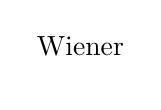
\begin{tikzpicture}

\begin{axis}[%
width=0.899202\figurewidth,
height=\figureheight,
at={(0\figurewidth,0\figureheight)},
scale only axis,
every outer x axis line/.append style={black},
every x tick label/.append style={font=\color{black}},
xtick={0,0.1},
xmin=0,
xmax=0.1,
xlabel={Frequency f/fs},
every outer y axis line/.append style={black},
every y tick label/.append style={font=\color{black}},
ymin=-80,
ymax=0,
title={Wiener},
axis x line*=bottom,
axis y line*=left
]
\addplot [color=black,solid,forget plot]
  table[row sep=crcr]{%
0.000244140625	-0.0268990251985883\\
0.00048828125	-0.0266313719953928\\
0.000732421875	-0.024196334554631\\
0.0009765625	-0.0277466784189073\\
0.001220703125	-0.0304334460414566\\
0.00146484375	-0.028768340595775\\
0.001708984375	-0.0269048798406857\\
0.001953125	-0.0224792372741831\\
0.002197265625	-0.026451875836301\\
0.00244140625	-0.0233326221382413\\
0.002685546875	-0.03219266341398\\
0.0029296875	-0.0283127453066641\\
0.003173828125	-0.0284485702256347\\
0.00341796875	-0.0309905882033377\\
0.003662109375	-0.0272170595091552\\
0.00390625	-0.0306677956976387\\
0.004150390625	-0.0299058857636396\\
0.00439453125	-0.030753627508318\\
0.004638671875	-0.036166757614069\\
0.0048828125	-0.0298326902157555\\
0.005126953125	-0.0398030881880231\\
0.00537109375	-0.0361606340314324\\
0.005615234375	-0.032637107426126\\
0.005859375	-0.0333663905918229\\
0.006103515625	-0.0363293771391113\\
0.00634765625	-0.0262834100905138\\
0.006591796875	-0.032933331382651\\
0.0068359375	-0.0410151535243131\\
0.007080078125	-0.0307747237459353\\
0.00732421875	-0.0409925436971434\\
0.007568359375	-0.0397875920839397\\
0.0078125	-0.0411336996853606\\
0.008056640625	-0.0382287037115816\\
0.00830078125	-0.0510539503461018\\
0.008544921875	-0.0475436945421279\\
0.0087890625	-0.0464456534008377\\
0.009033203125	-0.040123917609094\\
0.00927734375	-0.0495352138611338\\
0.009521484375	-0.0574719629629499\\
0.009765625	-0.0419762677072413\\
0.010009765625	-0.045776117567641\\
0.01025390625	-0.0609713647780268\\
0.010498046875	-0.0521386117709994\\
0.0107421875	-0.0563894235661451\\
0.010986328125	-0.0561900185091986\\
0.01123046875	-0.0596678474621513\\
0.011474609375	-0.0615958363605955\\
0.01171875	-0.0677023777940917\\
0.011962890625	-0.054921021669827\\
0.01220703125	-0.069533333515551\\
0.012451171875	-0.0610930331400255\\
0.0126953125	-0.0658029468465884\\
0.012939453125	-0.0705556920301547\\
0.01318359375	-0.0745777821961724\\
0.013427734375	-0.068614684603574\\
0.013671875	-0.0813167207492143\\
0.013916015625	-0.0750936140407816\\
0.01416015625	-0.077717634311341\\
0.014404296875	-0.0748064969811821\\
0.0146484375	-0.0763038046263773\\
0.014892578125	-0.0760025691840269\\
0.01513671875	-0.075872547073061\\
0.015380859375	-0.0809295409833908\\
0.015625	-0.0861101907365764\\
0.015869140625	-0.0803926397278474\\
0.01611328125	-0.0895753142235094\\
0.016357421875	-0.0960949788353105\\
0.0166015625	-0.0947726513138036\\
0.016845703125	-0.0997721005812764\\
0.01708984375	-0.106147505971819\\
0.017333984375	-0.105034234208745\\
0.017578125	-0.104320693530383\\
0.017822265625	-0.105514915167248\\
0.01806640625	-0.113987851145168\\
0.018310546875	-0.106849353484222\\
0.0185546875	-0.110155974673546\\
0.018798828125	-0.110986559638945\\
0.01904296875	-0.118892387089886\\
0.019287109375	-0.120538681767016\\
0.01953125	-0.120013856575497\\
0.019775390625	-0.122268106007994\\
0.02001953125	-0.131134811044205\\
0.020263671875	-0.13117780935886\\
0.0205078125	-0.130655596291092\\
0.020751953125	-0.13784190342875\\
0.02099609375	-0.134265991456004\\
0.021240234375	-0.142852462044743\\
0.021484375	-0.139103364627374\\
0.021728515625	-0.140517522781579\\
0.02197265625	-0.145356753622423\\
0.022216796875	-0.13954642782204\\
0.0224609375	-0.144977710375315\\
0.022705078125	-0.15211402389474\\
0.02294921875	-0.154662196990557\\
0.023193359375	-0.155921362970957\\
0.0234375	-0.160568798303814\\
0.023681640625	-0.164341531710022\\
0.02392578125	-0.169291633839009\\
0.024169921875	-0.170115594022889\\
0.0244140625	-0.167365848230588\\
0.024658203125	-0.169556433347964\\
0.02490234375	-0.176143011100862\\
0.025146484375	-0.179110643722538\\
0.025390625	-0.181548903497912\\
0.025634765625	-0.191104301245332\\
0.02587890625	-0.192190143340213\\
0.026123046875	-0.198157778222935\\
0.0263671875	-0.196521203354678\\
0.026611328125	-0.197994324904244\\
0.02685546875	-0.202729950366631\\
0.027099609375	-0.207954087249675\\
0.02734375	-0.202832668621966\\
0.027587890625	-0.209439585593259\\
0.02783203125	-0.214216294099799\\
0.028076171875	-0.218283495258049\\
0.0283203125	-0.225610146251256\\
0.028564453125	-0.225657686951251\\
0.02880859375	-0.227328128453109\\
0.029052734375	-0.238098716569823\\
0.029296875	-0.2367804433336\\
0.029541015625	-0.239761341670146\\
0.02978515625	-0.239081973918474\\
0.030029296875	-0.246634910265357\\
0.0302734375	-0.243431356363317\\
0.030517578125	-0.253208149568479\\
0.03076171875	-0.24639012534999\\
0.031005859375	-0.261783632113179\\
0.03125	-0.259106895942978\\
0.031494140625	-0.264066932623223\\
0.03173828125	-0.264528445892267\\
0.031982421875	-0.273082865956098\\
0.0322265625	-0.273129137170031\\
0.032470703125	-0.278682679221617\\
0.03271484375	-0.282598332670489\\
0.032958984375	-0.286817273194515\\
0.033203125	-0.28847499792937\\
0.033447265625	-0.288943215537245\\
0.03369140625	-0.291543019200049\\
0.033935546875	-0.301490965997914\\
0.0341796875	-0.303857708827366\\
0.034423828125	-0.316655997402222\\
0.03466796875	-0.318418558342387\\
0.034912109375	-0.319780096591842\\
0.03515625	-0.328073518326676\\
0.035400390625	-0.327386571114573\\
0.03564453125	-0.335401075712923\\
0.035888671875	-0.337170747402013\\
0.0361328125	-0.341555706096358\\
0.036376953125	-0.338960103223087\\
0.03662109375	-0.340283062167316\\
0.036865234375	-0.33935343124341\\
0.037109375	-0.357111413774987\\
0.037353515625	-0.360331544633709\\
0.03759765625	-0.360461686711517\\
0.037841796875	-0.368405359551446\\
0.0380859375	-0.368923227081893\\
0.038330078125	-0.383261548915357\\
0.03857421875	-0.383643094285333\\
0.038818359375	-0.389696209521219\\
0.0390625	-0.383045425508385\\
0.039306640625	-0.400718581255433\\
0.03955078125	-0.392944875738692\\
0.039794921875	-0.401848727285028\\
0.0400390625	-0.404273883511848\\
0.040283203125	-0.414634980173503\\
0.04052734375	-0.420206507712521\\
0.040771484375	-0.423178677839587\\
0.041015625	-0.432144892460485\\
0.041259765625	-0.433866379420294\\
0.04150390625	-0.432316656151727\\
0.041748046875	-0.437819677626123\\
0.0419921875	-0.451310199029649\\
0.042236328125	-0.44387768063558\\
0.04248046875	-0.444475240601889\\
0.042724609375	-0.455651429624993\\
0.04296875	-0.474093351620411\\
0.043212890625	-0.465655942358183\\
0.04345703125	-0.469514583283967\\
0.043701171875	-0.475508874270076\\
0.0439453125	-0.483604625637327\\
0.044189453125	-0.484516974808059\\
0.04443359375	-0.492926640662006\\
0.044677734375	-0.510455285758212\\
0.044921875	-0.500193859578985\\
0.045166015625	-0.50788857699996\\
0.04541015625	-0.516403492147447\\
0.045654296875	-0.518590716264043\\
0.0458984375	-0.517124317004857\\
0.046142578125	-0.521086644347292\\
0.04638671875	-0.536582879579555\\
0.046630859375	-0.533541783534531\\
0.046875	-0.540859826177041\\
0.047119140625	-0.548291929050151\\
0.04736328125	-0.553665858701493\\
0.047607421875	-0.559040416198968\\
0.0478515625	-0.560686519822468\\
0.048095703125	-0.57081946294926\\
0.04833984375	-0.57344288319058\\
0.048583984375	-0.584152752347734\\
0.048828125	-0.58541662893424\\
0.049072265625	-0.588948975242999\\
0.04931640625	-0.602520582343232\\
0.049560546875	-0.600662627741258\\
0.0498046875	-0.607036245409461\\
0.050048828125	-0.606059336939552\\
0.05029296875	-0.612649705703291\\
0.050537109375	-0.616431797401049\\
0.05078125	-0.628794732516553\\
0.051025390625	-0.634946375302661\\
0.05126953125	-0.636312673518319\\
0.051513671875	-0.635376561263911\\
0.0517578125	-0.653228720992786\\
0.052001953125	-0.65610608911328\\
0.05224609375	-0.662437262204776\\
0.052490234375	-0.665153345205965\\
0.052734375	-0.673883210319161\\
0.052978515625	-0.679477158323266\\
0.05322265625	-0.6839885374348\\
0.053466796875	-0.694561395443145\\
0.0537109375	-0.685106357416316\\
0.053955078125	-0.704866346191352\\
0.05419921875	-0.707284333996256\\
0.054443359375	-0.70598945571129\\
0.0546875	-0.716506957637023\\
0.054931640625	-0.723742711443492\\
0.05517578125	-0.735315688534229\\
0.055419921875	-0.727889287421192\\
0.0556640625	-0.744123808361735\\
0.055908203125	-0.745706822872535\\
0.05615234375	-0.756247454636309\\
0.056396484375	-0.762394853916078\\
0.056640625	-0.772092327633686\\
0.056884765625	-0.766172554185516\\
0.05712890625	-0.778186029522658\\
0.057373046875	-0.775157298306851\\
0.0576171875	-0.787757828191161\\
0.057861328125	-0.788483233405543\\
0.05810546875	-0.806156601170244\\
0.058349609375	-0.804183500478189\\
0.05859375	-0.823325305903722\\
0.058837890625	-0.81334507862897\\
0.05908203125	-0.830206037172502\\
0.059326171875	-0.835982540653845\\
0.0595703125	-0.837739320406797\\
0.059814453125	-0.844720287577672\\
0.06005859375	-0.850940373806054\\
0.060302734375	-0.858339589389743\\
0.060546875	-0.860867451900049\\
0.060791015625	-0.870277758957002\\
0.06103515625	-0.883032173796948\\
0.061279296875	-0.878484171835851\\
0.0615234375	-0.882618140728823\\
0.061767578125	-0.893828501113376\\
0.06201171875	-0.901721749033072\\
0.062255859375	-0.906723606130186\\
0.0625	-0.911077628990029\\
0.062744140625	-0.91910480370916\\
0.06298828125	-0.926584996871327\\
0.063232421875	-0.932167837445149\\
0.0634765625	-0.94614199656462\\
0.063720703125	-0.943358940518806\\
0.06396484375	-0.94307000876654\\
0.064208984375	-0.96889111765978\\
0.064453125	-0.967026528092845\\
0.064697265625	-0.975655536450802\\
0.06494140625	-0.983608950897462\\
0.065185546875	-0.989111653603686\\
0.0654296875	-0.994438188307072\\
0.065673828125	-1.00244920685049\\
0.06591796875	-1.00635073727722\\
0.066162109375	-1.01199974482648\\
0.06640625	-1.01553138911021\\
0.066650390625	-1.0280182614805\\
0.06689453125	-1.03808218877259\\
0.067138671875	-1.03879015226727\\
0.0673828125	-1.04686735351129\\
0.067626953125	-1.04928365919\\
0.06787109375	-1.06325411732564\\
0.068115234375	-1.0682349309397\\
0.068359375	-1.06959883814318\\
0.068603515625	-1.0822973638011\\
0.06884765625	-1.08131129412493\\
0.069091796875	-1.09509332910886\\
0.0693359375	-1.0993720015739\\
0.069580078125	-1.11007664769147\\
0.06982421875	-1.11502559185317\\
0.070068359375	-1.12017018371904\\
0.0703125	-1.12469060679734\\
0.070556640625	-1.13634147094115\\
0.07080078125	-1.14634696104577\\
0.071044921875	-1.15480509581118\\
0.0712890625	-1.15413786222302\\
0.071533203125	-1.16235895412342\\
0.07177734375	-1.16353295395436\\
0.072021484375	-1.18025148242754\\
0.072265625	-1.18975634811142\\
0.072509765625	-1.19747124862857\\
0.07275390625	-1.1977259862287\\
0.072998046875	-1.21010567074688\\
0.0732421875	-1.21076194803123\\
0.073486328125	-1.21550808552263\\
0.07373046875	-1.22929191283498\\
0.073974609375	-1.23732591399124\\
0.07421875	-1.24406402543968\\
0.074462890625	-1.24833578410903\\
0.07470703125	-1.25499343042696\\
0.074951171875	-1.24859246875423\\
0.0751953125	-1.27984319977395\\
0.075439453125	-1.28162331022446\\
0.07568359375	-1.28664636902437\\
0.075927734375	-1.29922921413896\\
0.076171875	-1.30765820893447\\
0.076416015625	-1.30987576184316\\
0.07666015625	-1.31253980091685\\
0.076904296875	-1.32629091291852\\
0.0771484375	-1.32796587571488\\
0.077392578125	-1.33795268285979\\
0.07763671875	-1.34255155509538\\
0.077880859375	-1.35485019267082\\
0.078125	-1.35790371832132\\
0.078369140625	-1.36708156292008\\
0.07861328125	-1.37620056591379\\
0.078857421875	-1.37943727156801\\
0.0791015625	-1.38933024506156\\
0.079345703125	-1.40115470093048\\
0.07958984375	-1.40483946045543\\
0.079833984375	-1.41171656436507\\
0.080078125	-1.41790353574851\\
0.080322265625	-1.43324399728522\\
0.08056640625	-1.43542383869539\\
0.080810546875	-1.44486316257064\\
0.0810546875	-1.45132321481378\\
0.081298828125	-1.4494299957621\\
0.08154296875	-1.46689451829849\\
0.081787109375	-1.47239818839364\\
0.08203125	-1.4851153143133\\
0.082275390625	-1.4817172273606\\
0.08251953125	-1.50049899160109\\
0.082763671875	-1.49307787737791\\
0.0830078125	-1.51300073150117\\
0.083251953125	-1.52717933871548\\
0.08349609375	-1.52943152665114\\
0.083740234375	-1.53411484825943\\
0.083984375	-1.53620918316886\\
0.084228515625	-1.54327363173866\\
0.08447265625	-1.56020042101045\\
0.084716796875	-1.56624136800735\\
0.0849609375	-1.58001047151237\\
0.085205078125	-1.58239831255003\\
0.08544921875	-1.59253522729711\\
0.085693359375	-1.59723041174141\\
0.0859375	-1.60714689921019\\
0.086181640625	-1.61713385056805\\
0.08642578125	-1.61582091097586\\
0.086669921875	-1.63353516366374\\
0.0869140625	-1.63272691956644\\
0.087158203125	-1.64993798826549\\
0.08740234375	-1.65325036746714\\
0.087646484375	-1.65839003857144\\
0.087890625	-1.66642322030788\\
0.088134765625	-1.67681797046276\\
0.08837890625	-1.68664966975643\\
0.088623046875	-1.69132669198854\\
0.0888671875	-1.70673806360384\\
0.089111328125	-1.7120502167129\\
0.08935546875	-1.71628372565959\\
0.089599609375	-1.72287936096723\\
0.08984375	-1.72891967598099\\
0.090087890625	-1.73952597823359\\
0.09033203125	-1.75179460840519\\
0.090576171875	-1.75958680369263\\
0.0908203125	-1.77511538743966\\
0.091064453125	-1.77649539125076\\
0.09130859375	-1.78624623260202\\
0.091552734375	-1.79360698168284\\
0.091796875	-1.80591914910474\\
0.092041015625	-1.80967950611785\\
0.09228515625	-1.8174887507048\\
0.092529296875	-1.82797649692446\\
0.0927734375	-1.83766888906212\\
0.093017578125	-1.83942445123137\\
0.09326171875	-1.85401178995539\\
0.093505859375	-1.85991376996549\\
0.09375	-1.86902646590698\\
0.093994140625	-1.87715778587273\\
0.09423828125	-1.87479307166552\\
0.094482421875	-1.88715800960654\\
0.0947265625	-1.9038436790679\\
0.094970703125	-1.90870828771961\\
0.09521484375	-1.91610297255704\\
0.095458984375	-1.92455555751434\\
0.095703125	-1.93520208871092\\
0.095947265625	-1.94497411637957\\
0.09619140625	-1.95471195793658\\
0.096435546875	-1.95645991424027\\
0.0966796875	-1.96807895237203\\
0.096923828125	-1.9794147389461\\
0.09716796875	-1.98216852125341\\
0.097412109375	-1.98912281388021\\
0.09765625	-1.99893519918828\\
0.097900390625	-2.00505584377902\\
0.09814453125	-2.01501721603029\\
0.098388671875	-2.01867526479737\\
0.0986328125	-2.03360287570433\\
0.098876953125	-2.04155555578848\\
0.09912109375	-2.04955588045351\\
0.099365234375	-2.06081239140644\\
0.099609375	-2.06437160901146\\
0.099853515625	-2.08765306360402\\
};
\addplot [color=blue,solid,forget plot]
  table[row sep=crcr]{%
0.000244140625	-53.8784348337131\\
0.00048828125	-54.8525756401823\\
0.000732421875	-55.288282625768\\
0.0009765625	-55.4403131652681\\
0.001220703125	-53.5224925822404\\
0.00146484375	-55.1058818314117\\
0.001708984375	-57.0388386276866\\
0.001953125	-54.1778839124116\\
0.002197265625	-52.6631343872772\\
0.00244140625	-51.3481390255117\\
0.002685546875	-53.8008123691667\\
0.0029296875	-51.9046925278799\\
0.003173828125	-52.1968455857261\\
0.00341796875	-55.8363622900919\\
0.003662109375	-54.1011361668977\\
0.00390625	-53.3603631612056\\
0.004150390625	-52.4997823444883\\
0.00439453125	-52.8744067296813\\
0.004638671875	-53.4427173634807\\
0.0048828125	-54.469813544182\\
0.005126953125	-58.0998123430072\\
0.00537109375	-54.4946950004931\\
0.005615234375	-55.373544406907\\
0.005859375	-53.1732778598026\\
0.006103515625	-52.6425086052251\\
0.00634765625	-53.8069358668692\\
0.006591796875	-53.5258710344074\\
0.0068359375	-54.7853875919884\\
0.007080078125	-52.3693831983685\\
0.00732421875	-51.9395649177693\\
0.007568359375	-53.6423737490604\\
0.0078125	-56.5703739083117\\
0.008056640625	-58.1357883004675\\
0.00830078125	-54.6170824761863\\
0.008544921875	-53.8935901332732\\
0.0087890625	-55.1065562891114\\
0.009033203125	-54.3598009235389\\
0.00927734375	-53.4188860797603\\
0.009521484375	-52.599146490422\\
0.009765625	-51.9331446595714\\
0.010009765625	-53.794530707001\\
0.01025390625	-52.3538893794097\\
0.010498046875	-52.5727969903\\
0.0107421875	-52.9769431807755\\
0.010986328125	-53.7711984173069\\
0.01123046875	-53.29474849634\\
0.011474609375	-52.8649476531187\\
0.01171875	-51.1419473978657\\
0.011962890625	-55.7483410804082\\
0.01220703125	-54.0191244030322\\
0.012451171875	-52.5876910713431\\
0.0126953125	-54.6013162988796\\
0.012939453125	-55.1711992313422\\
0.01318359375	-52.3952436662911\\
0.013427734375	-51.4388193859806\\
0.013671875	-54.4141586839582\\
0.013916015625	-57.1785367349569\\
0.01416015625	-51.9622084538479\\
0.014404296875	-54.4158991994356\\
0.0146484375	-54.5489664885307\\
0.014892578125	-55.2058142618249\\
0.01513671875	-55.6932381521653\\
0.015380859375	-54.1109743240974\\
0.015625	-55.5595520004971\\
0.015869140625	-52.8840557346269\\
0.01611328125	-53.2606130335407\\
0.016357421875	-54.3150376615963\\
0.0166015625	-53.2177208769891\\
0.016845703125	-53.9680653630891\\
0.01708984375	-56.7277711180464\\
0.017333984375	-51.3672509313477\\
0.017578125	-50.5538990631017\\
0.017822265625	-53.0970442124783\\
0.01806640625	-55.4975898517285\\
0.018310546875	-55.4485912726317\\
0.0185546875	-52.5661256796734\\
0.018798828125	-52.9330391719632\\
0.01904296875	-52.0139690949943\\
0.019287109375	-54.6232598965122\\
0.01953125	-53.4489400713875\\
0.019775390625	-55.4375737448858\\
0.02001953125	-54.9474221045545\\
0.020263671875	-52.6891067232809\\
0.0205078125	-55.4644163771152\\
0.020751953125	-52.2270856185481\\
0.02099609375	-55.4533901901955\\
0.021240234375	-55.1974160888742\\
0.021484375	-50.545437983338\\
0.021728515625	-55.6852219923671\\
0.02197265625	-54.4088249257398\\
0.022216796875	-56.3290990128532\\
0.0224609375	-55.3829727399332\\
0.022705078125	-53.6489198735316\\
0.02294921875	-55.4692053998817\\
0.023193359375	-55.0058232839743\\
0.0234375	-53.8801685656596\\
0.023681640625	-53.8057812818609\\
0.02392578125	-51.2259658078794\\
0.024169921875	-52.9091892753931\\
0.0244140625	-56.2287165913976\\
0.024658203125	-53.6141292304178\\
0.02490234375	-53.0336904882909\\
0.025146484375	-54.6280318884711\\
0.025390625	-53.156745923971\\
0.025634765625	-53.3278627537076\\
0.02587890625	-55.5784548382794\\
0.026123046875	-51.814440146233\\
0.0263671875	-53.4022244844452\\
0.026611328125	-54.2454824472758\\
0.02685546875	-55.883656831698\\
0.027099609375	-53.2737922948977\\
0.02734375	-55.1160439707818\\
0.027587890625	-53.6946041665326\\
0.02783203125	-54.1672480596172\\
0.028076171875	-53.3980181070313\\
0.0283203125	-52.4744731153142\\
0.028564453125	-53.3210707799365\\
0.02880859375	-53.9030122393089\\
0.029052734375	-53.1508870643759\\
0.029296875	-50.5748836219158\\
0.029541015625	-54.4405578584673\\
0.02978515625	-56.0904822413239\\
0.030029296875	-54.5067627266152\\
0.0302734375	-51.4573600084703\\
0.030517578125	-57.0422286955239\\
0.03076171875	-54.3670146232926\\
0.031005859375	-53.2515016116588\\
0.03125	-51.2056429253407\\
0.031494140625	-54.3204025038096\\
0.03173828125	-55.5051206246061\\
0.031982421875	-54.4440393276361\\
0.0322265625	-54.4158816738249\\
0.032470703125	-54.8021788907369\\
0.03271484375	-55.5860684501359\\
0.032958984375	-55.3558669652614\\
0.033203125	-56.0120158214702\\
0.033447265625	-56.6252677359103\\
0.03369140625	-56.4067390115187\\
0.033935546875	-52.7555344747383\\
0.0341796875	-52.0417257450208\\
0.034423828125	-55.186627085794\\
0.03466796875	-55.3213816183853\\
0.034912109375	-55.1520206635709\\
0.03515625	-53.3665969171389\\
0.035400390625	-54.4514882586383\\
0.03564453125	-54.1350039436471\\
0.035888671875	-56.8619155474954\\
0.0361328125	-56.3785912760883\\
0.036376953125	-52.8849963215248\\
0.03662109375	-55.2747742127194\\
0.036865234375	-54.8404512883298\\
0.037109375	-54.5443811026765\\
0.037353515625	-53.9450832397413\\
0.03759765625	-54.761122571229\\
0.037841796875	-56.6663637281208\\
0.0380859375	-55.1609186819161\\
0.038330078125	-55.0702554729202\\
0.03857421875	-53.0389333922465\\
0.038818359375	-53.3660371974\\
0.0390625	-53.6890612503748\\
0.039306640625	-52.6390525403118\\
0.03955078125	-54.0298192170209\\
0.039794921875	-54.5436875498363\\
0.0400390625	-55.212155264118\\
0.040283203125	-54.5844988511201\\
0.04052734375	-51.4693020313129\\
0.040771484375	-54.5564561834402\\
0.041015625	-54.2193876314682\\
0.041259765625	-56.9301448422873\\
0.04150390625	-55.0474934889353\\
0.041748046875	-54.4313937264992\\
0.0419921875	-55.3348437313047\\
0.042236328125	-52.9151842150604\\
0.04248046875	-55.6491670047391\\
0.042724609375	-53.172581732775\\
0.04296875	-55.6764196848727\\
0.043212890625	-53.5244017485301\\
0.04345703125	-53.2410962671119\\
0.043701171875	-55.4375458203076\\
0.0439453125	-55.2872748733061\\
0.044189453125	-56.846336909213\\
0.04443359375	-52.8465640473575\\
0.044677734375	-52.4205619684465\\
0.044921875	-55.3553714543091\\
0.045166015625	-55.0404033473722\\
0.04541015625	-52.7240405697065\\
0.045654296875	-53.6641874664489\\
0.0458984375	-54.8608606674558\\
0.046142578125	-55.7435247160648\\
0.04638671875	-56.7461829271591\\
0.046630859375	-54.1559292333394\\
0.046875	-55.0934643771159\\
0.047119140625	-53.6700236958017\\
0.04736328125	-54.2842286606233\\
0.047607421875	-54.6324699968289\\
0.0478515625	-54.178213760535\\
0.048095703125	-54.9839670469075\\
0.04833984375	-54.1565850337342\\
0.048583984375	-53.8702149539918\\
0.048828125	-55.6284061489178\\
0.049072265625	-52.0438608323286\\
0.04931640625	-54.4562192328928\\
0.049560546875	-54.4565589468917\\
0.0498046875	-56.0662353802029\\
0.050048828125	-57.2194334708649\\
0.05029296875	-52.5365968456642\\
0.050537109375	-53.8218536777679\\
0.05078125	-52.677479960429\\
0.051025390625	-57.9848328274016\\
0.05126953125	-55.7904112938541\\
0.051513671875	-57.3864822282677\\
0.0517578125	-55.4427838477998\\
0.052001953125	-54.2581779942792\\
0.05224609375	-50.5189049131889\\
0.052490234375	-53.2174944136171\\
0.052734375	-53.426052357997\\
0.052978515625	-55.8275533094076\\
0.05322265625	-51.8419774718865\\
0.053466796875	-55.3205730315842\\
0.0537109375	-53.0744366586834\\
0.053955078125	-57.731890424504\\
0.05419921875	-52.5285147869115\\
0.054443359375	-52.8732985192745\\
0.0546875	-53.7384166681647\\
0.054931640625	-57.0752599943849\\
0.05517578125	-53.7877727665206\\
0.055419921875	-55.1012930595208\\
0.0556640625	-55.88311049298\\
0.055908203125	-57.254460537384\\
0.05615234375	-54.2345282791233\\
0.056396484375	-53.375610730466\\
0.056640625	-55.0132734562498\\
0.056884765625	-54.6926772974301\\
0.05712890625	-52.4818852681148\\
0.057373046875	-53.3536257221398\\
0.0576171875	-53.3956962028853\\
0.057861328125	-54.8700908263754\\
0.05810546875	-54.4182425667761\\
0.058349609375	-53.2733745834238\\
0.05859375	-56.6497979191403\\
0.058837890625	-52.9491039285951\\
0.05908203125	-53.9741725306388\\
0.059326171875	-53.6418440543415\\
0.0595703125	-56.7855718074982\\
0.059814453125	-55.9056447329201\\
0.06005859375	-54.7931030443393\\
0.060302734375	-52.5528993307645\\
0.060546875	-55.9618961759579\\
0.060791015625	-54.7978353473602\\
0.06103515625	-57.5231624297682\\
0.061279296875	-56.5181130219059\\
0.0615234375	-53.9639728538355\\
0.061767578125	-55.2481282646714\\
0.06201171875	-53.1009915850276\\
0.062255859375	-55.0366685618173\\
0.0625	-54.8013138704835\\
0.062744140625	-52.1798497382877\\
0.06298828125	-53.8917678354033\\
0.063232421875	-55.4190174076463\\
0.0634765625	-56.921452634001\\
0.063720703125	-53.5606614511711\\
0.06396484375	-53.8008600173829\\
0.064208984375	-54.1204559503089\\
0.064453125	-55.4508885744972\\
0.064697265625	-54.2551765141347\\
0.06494140625	-55.4378950082506\\
0.065185546875	-54.3007125565248\\
0.0654296875	-52.7957724741523\\
0.065673828125	-55.5170443370749\\
0.06591796875	-55.8191144469525\\
0.066162109375	-53.1627194755715\\
0.06640625	-56.3023103476661\\
0.066650390625	-53.7652190030078\\
0.06689453125	-56.3660418786315\\
0.067138671875	-54.333466774643\\
0.0673828125	-55.1703841328525\\
0.067626953125	-55.9950139349654\\
0.06787109375	-54.8605227462394\\
0.068115234375	-52.4526146181927\\
0.068359375	-55.5892627781691\\
0.068603515625	-54.938029602369\\
0.06884765625	-55.3081518584345\\
0.069091796875	-54.2475814370281\\
0.0693359375	-54.0679224333228\\
0.069580078125	-55.3788304701316\\
0.06982421875	-53.1676268133606\\
0.070068359375	-52.5199958214646\\
0.0703125	-56.7383733280532\\
0.070556640625	-57.1417923910814\\
0.07080078125	-55.7492146180022\\
0.071044921875	-55.7304943060302\\
0.0712890625	-58.2318270473524\\
0.071533203125	-57.3265172943647\\
0.07177734375	-53.246332011371\\
0.072021484375	-51.5497593617589\\
0.072265625	-55.905699351598\\
0.072509765625	-56.6325045097702\\
0.07275390625	-52.3918615329584\\
0.072998046875	-56.3024134730324\\
0.0732421875	-56.0467753131102\\
0.073486328125	-52.2918078095972\\
0.07373046875	-53.6263497259659\\
0.073974609375	-56.6128631191834\\
0.07421875	-54.4897219184875\\
0.074462890625	-55.2133891058469\\
0.07470703125	-55.5846804256014\\
0.074951171875	-54.8902096587184\\
0.0751953125	-54.85491797134\\
0.075439453125	-53.3241181737085\\
0.07568359375	-55.1880599061719\\
0.075927734375	-53.1550546038736\\
0.076171875	-52.6383477219884\\
0.076416015625	-53.7906981402387\\
0.07666015625	-54.220720145177\\
0.076904296875	-54.8740277870721\\
0.0771484375	-54.0355755866169\\
0.077392578125	-55.4932953774424\\
0.07763671875	-56.2563301016764\\
0.077880859375	-54.59522357605\\
0.078125	-53.156930839823\\
0.078369140625	-55.2050651407545\\
0.07861328125	-53.1711188741939\\
0.078857421875	-56.612247793001\\
0.0791015625	-57.3394581531103\\
0.079345703125	-54.6141915525973\\
0.07958984375	-57.7242032065353\\
0.079833984375	-56.9050306777176\\
0.080078125	-55.1166987619566\\
0.080322265625	-54.2684987466805\\
0.08056640625	-55.976010967275\\
0.080810546875	-54.3322247912335\\
0.0810546875	-56.6977347069553\\
0.081298828125	-54.8995104928955\\
0.08154296875	-56.6584319727035\\
0.081787109375	-55.7960843528676\\
0.08203125	-54.1958769156049\\
0.082275390625	-55.3040803617358\\
0.08251953125	-52.5205212568359\\
0.082763671875	-55.6688988700723\\
0.0830078125	-57.1698338253136\\
0.083251953125	-55.1802357441352\\
0.08349609375	-56.4962597211701\\
0.083740234375	-59.2722393440201\\
0.083984375	-59.0306178478417\\
0.084228515625	-62.1612275676239\\
0.08447265625	-54.6669237898542\\
0.084716796875	-54.0285846443007\\
0.0849609375	-54.9764260144393\\
0.085205078125	-55.6507177198766\\
0.08544921875	-54.265374010902\\
0.085693359375	-54.9590493114611\\
0.0859375	-53.728101587298\\
0.086181640625	-56.5413276086559\\
0.08642578125	-56.6332715590462\\
0.086669921875	-55.2292019279428\\
0.0869140625	-54.2658411155241\\
0.087158203125	-54.9704006776233\\
0.08740234375	-53.1568577478277\\
0.087646484375	-55.0324686048926\\
0.087890625	-54.9291200353109\\
0.088134765625	-57.0280227084036\\
0.08837890625	-56.6193821207463\\
0.088623046875	-56.3635096321585\\
0.0888671875	-53.6299538714551\\
0.089111328125	-58.273865289041\\
0.08935546875	-55.4897616491374\\
0.089599609375	-54.0567512447928\\
0.08984375	-59.5792826612287\\
0.090087890625	-57.0086161537064\\
0.09033203125	-58.014398946407\\
0.090576171875	-57.7310563345563\\
0.0908203125	-56.3306960814763\\
0.091064453125	-55.1864380140353\\
0.09130859375	-56.6222108952312\\
0.091552734375	-56.875956554554\\
0.091796875	-56.9562431325164\\
0.092041015625	-55.7377234868611\\
0.09228515625	-52.3638887544162\\
0.092529296875	-54.083133767165\\
0.0927734375	-56.3876300282207\\
0.093017578125	-61.1038434952526\\
0.09326171875	-57.0753508812373\\
0.093505859375	-56.823545641362\\
0.09375	-55.3180195824305\\
0.093994140625	-57.1915147883074\\
0.09423828125	-54.3087112254942\\
0.094482421875	-52.566685961383\\
0.0947265625	-57.2123153381826\\
0.094970703125	-56.5706660703719\\
0.09521484375	-56.3223428003685\\
0.095458984375	-54.3139644762165\\
0.095703125	-54.5983786860446\\
0.095947265625	-56.3910908174589\\
0.09619140625	-54.3013967391479\\
0.096435546875	-58.0086700971407\\
0.0966796875	-55.5980350189639\\
0.096923828125	-56.8016165184947\\
0.09716796875	-53.9139870496481\\
0.097412109375	-55.0097864977906\\
0.09765625	-54.0007173798396\\
0.097900390625	-56.632748925472\\
0.09814453125	-57.378452360133\\
0.098388671875	-55.5750190938871\\
0.0986328125	-55.9632301813043\\
0.098876953125	-55.3807364876162\\
0.09912109375	-57.3153405710292\\
0.099365234375	-54.7998936889032\\
0.099609375	-54.7771531056356\\
0.099853515625	-55.2202488521334\\
};
\addplot [color=red,solid,forget plot]
  table[row sep=crcr]{%
0.000244140625	-63.8784348337131\\
0.00048828125	-64.8525756401823\\
0.000732421875	-65.288282625768\\
0.0009765625	-65.4403131652681\\
0.001220703125	-63.5224925822404\\
0.00146484375	-65.1058818314117\\
0.001708984375	-67.0388386276866\\
0.001953125	-64.1778839124116\\
0.002197265625	-62.6631343872772\\
0.00244140625	-61.3481390255117\\
0.002685546875	-63.8008123691667\\
0.0029296875	-61.9046925278799\\
0.003173828125	-62.1968455857261\\
0.00341796875	-65.8363622900919\\
0.003662109375	-64.1011361668977\\
0.00390625	-63.3603631612056\\
0.004150390625	-62.4997823444883\\
0.00439453125	-62.8744067296813\\
0.004638671875	-63.4427173634807\\
0.0048828125	-64.469813544182\\
0.005126953125	-68.0998123430072\\
0.00537109375	-64.4946950004931\\
0.005615234375	-65.373544406907\\
0.005859375	-63.1732778598026\\
0.006103515625	-62.6425086052251\\
0.00634765625	-63.8069358668692\\
0.006591796875	-63.5258710344074\\
0.0068359375	-64.7853875919884\\
0.007080078125	-62.3693831983685\\
0.00732421875	-61.9395649177693\\
0.007568359375	-63.6423737490604\\
0.0078125	-66.5703739083117\\
0.008056640625	-68.1357883004675\\
0.00830078125	-64.6170824761863\\
0.008544921875	-63.8935901332732\\
0.0087890625	-65.1065562891114\\
0.009033203125	-64.3598009235389\\
0.00927734375	-63.4188860797603\\
0.009521484375	-62.599146490422\\
0.009765625	-61.9331446595714\\
0.010009765625	-63.794530707001\\
0.01025390625	-62.3538893794097\\
0.010498046875	-62.5727969903\\
0.0107421875	-62.9769431807755\\
0.010986328125	-63.7711984173069\\
0.01123046875	-63.29474849634\\
0.011474609375	-62.8649476531187\\
0.01171875	-61.1419473978657\\
0.011962890625	-65.7483410804082\\
0.01220703125	-64.0191244030322\\
0.012451171875	-62.5876910713431\\
0.0126953125	-64.6013162988796\\
0.012939453125	-65.1711992313422\\
0.01318359375	-62.3952436662911\\
0.013427734375	-61.4388193859806\\
0.013671875	-64.4141586839582\\
0.013916015625	-67.1785367349569\\
0.01416015625	-61.9622084538479\\
0.014404296875	-64.4158991994356\\
0.0146484375	-64.5489664885307\\
0.014892578125	-65.2058142618249\\
0.01513671875	-65.6932381521653\\
0.015380859375	-64.1109743240974\\
0.015625	-65.5595520004971\\
0.015869140625	-62.8840557346269\\
0.01611328125	-63.2606130335407\\
0.016357421875	-64.3150376615963\\
0.0166015625	-63.2177208769891\\
0.016845703125	-63.9680653630891\\
0.01708984375	-66.7277711180465\\
0.017333984375	-61.3672509313477\\
0.017578125	-60.5538990631017\\
0.017822265625	-63.0970442124783\\
0.01806640625	-65.4975898517285\\
0.018310546875	-65.4485912726317\\
0.0185546875	-62.5661256796734\\
0.018798828125	-62.9330391719632\\
0.01904296875	-62.0139690949943\\
0.019287109375	-64.6232598965122\\
0.01953125	-63.4489400713875\\
0.019775390625	-65.4375737448858\\
0.02001953125	-64.9474221045545\\
0.020263671875	-62.6891067232809\\
0.0205078125	-65.4644163771152\\
0.020751953125	-62.2270856185481\\
0.02099609375	-65.4533901901955\\
0.021240234375	-65.1974160888742\\
0.021484375	-60.545437983338\\
0.021728515625	-65.6852219923671\\
0.02197265625	-64.4088249257398\\
0.022216796875	-66.3290990128532\\
0.0224609375	-65.3829727399332\\
0.022705078125	-63.6489198735316\\
0.02294921875	-65.4692053998817\\
0.023193359375	-65.0058232839743\\
0.0234375	-63.8801685656596\\
0.023681640625	-63.8057812818609\\
0.02392578125	-61.2259658078794\\
0.024169921875	-62.9091892753931\\
0.0244140625	-66.2287165913976\\
0.024658203125	-63.6141292304178\\
0.02490234375	-63.0336904882909\\
0.025146484375	-64.6280318884711\\
0.025390625	-63.156745923971\\
0.025634765625	-63.3278627537076\\
0.02587890625	-65.5784548382794\\
0.026123046875	-61.814440146233\\
0.0263671875	-63.4022244844452\\
0.026611328125	-64.2454824472758\\
0.02685546875	-65.883656831698\\
0.027099609375	-63.2737922948977\\
0.02734375	-65.1160439707818\\
0.027587890625	-63.6946041665326\\
0.02783203125	-64.1672480596172\\
0.028076171875	-63.3980181070313\\
0.0283203125	-62.4744731153142\\
0.028564453125	-63.3210707799365\\
0.02880859375	-63.9030122393089\\
0.029052734375	-63.1508870643759\\
0.029296875	-60.5748836219158\\
0.029541015625	-64.4405578584673\\
0.02978515625	-66.0904822413239\\
0.030029296875	-64.5067627266152\\
0.0302734375	-61.4573600084703\\
0.030517578125	-67.0422286955239\\
0.03076171875	-64.3670146232926\\
0.031005859375	-63.2515016116588\\
0.03125	-61.2056429253407\\
0.031494140625	-64.3204025038096\\
0.03173828125	-65.5051206246061\\
0.031982421875	-64.4440393276361\\
0.0322265625	-64.4158816738249\\
0.032470703125	-64.8021788907369\\
0.03271484375	-65.5860684501359\\
0.032958984375	-65.3558669652614\\
0.033203125	-66.0120158214702\\
0.033447265625	-66.6252677359103\\
0.03369140625	-66.4067390115187\\
0.033935546875	-62.7555344747383\\
0.0341796875	-62.0417257450208\\
0.034423828125	-65.186627085794\\
0.03466796875	-65.3213816183853\\
0.034912109375	-65.1520206635709\\
0.03515625	-63.3665969171389\\
0.035400390625	-64.4514882586383\\
0.03564453125	-64.1350039436471\\
0.035888671875	-66.8619155474954\\
0.0361328125	-66.3785912760883\\
0.036376953125	-62.8849963215248\\
0.03662109375	-65.2747742127194\\
0.036865234375	-64.8404512883298\\
0.037109375	-64.5443811026764\\
0.037353515625	-63.9450832397413\\
0.03759765625	-64.761122571229\\
0.037841796875	-66.6663637281208\\
0.0380859375	-65.1609186819161\\
0.038330078125	-65.0702554729202\\
0.03857421875	-63.0389333922465\\
0.038818359375	-63.3660371974\\
0.0390625	-63.6890612503748\\
0.039306640625	-62.6390525403118\\
0.03955078125	-64.0298192170209\\
0.039794921875	-64.5436875498363\\
0.0400390625	-65.212155264118\\
0.040283203125	-64.5844988511201\\
0.04052734375	-61.4693020313129\\
0.040771484375	-64.5564561834402\\
0.041015625	-64.2193876314682\\
0.041259765625	-66.9301448422872\\
0.04150390625	-65.0474934889353\\
0.041748046875	-64.4313937264992\\
0.0419921875	-65.3348437313047\\
0.042236328125	-62.9151842150604\\
0.04248046875	-65.6491670047391\\
0.042724609375	-63.172581732775\\
0.04296875	-65.6764196848727\\
0.043212890625	-63.5244017485301\\
0.04345703125	-63.2410962671119\\
0.043701171875	-65.4375458203076\\
0.0439453125	-65.2872748733061\\
0.044189453125	-66.846336909213\\
0.04443359375	-62.8465640473575\\
0.044677734375	-62.4205619684465\\
0.044921875	-65.3553714543091\\
0.045166015625	-65.0404033473722\\
0.04541015625	-62.7240405697065\\
0.045654296875	-63.6641874664489\\
0.0458984375	-64.8608606674558\\
0.046142578125	-65.7435247160648\\
0.04638671875	-66.7461829271591\\
0.046630859375	-64.1559292333394\\
0.046875	-65.0934643771159\\
0.047119140625	-63.6700236958017\\
0.04736328125	-64.2842286606233\\
0.047607421875	-64.6324699968289\\
0.0478515625	-64.178213760535\\
0.048095703125	-64.9839670469075\\
0.04833984375	-64.1565850337342\\
0.048583984375	-63.8702149539918\\
0.048828125	-65.6284061489178\\
0.049072265625	-62.0438608323286\\
0.04931640625	-64.4562192328928\\
0.049560546875	-64.4565589468917\\
0.0498046875	-66.0662353802029\\
0.050048828125	-67.2194334708649\\
0.05029296875	-62.5365968456642\\
0.050537109375	-63.8218536777679\\
0.05078125	-62.677479960429\\
0.051025390625	-67.9848328274016\\
0.05126953125	-65.7904112938541\\
0.051513671875	-67.3864822282677\\
0.0517578125	-65.4427838477998\\
0.052001953125	-64.2581779942792\\
0.05224609375	-60.5189049131889\\
0.052490234375	-63.2174944136171\\
0.052734375	-63.426052357997\\
0.052978515625	-65.8275533094076\\
0.05322265625	-61.8419774718865\\
0.053466796875	-65.3205730315843\\
0.0537109375	-63.0744366586834\\
0.053955078125	-67.731890424504\\
0.05419921875	-62.5285147869115\\
0.054443359375	-62.8732985192745\\
0.0546875	-63.7384166681647\\
0.054931640625	-67.0752599943849\\
0.05517578125	-63.7877727665206\\
0.055419921875	-65.1012930595208\\
0.0556640625	-65.88311049298\\
0.055908203125	-67.254460537384\\
0.05615234375	-64.2345282791233\\
0.056396484375	-63.375610730466\\
0.056640625	-65.0132734562498\\
0.056884765625	-64.6926772974301\\
0.05712890625	-62.4818852681148\\
0.057373046875	-63.3536257221398\\
0.0576171875	-63.3956962028853\\
0.057861328125	-64.8700908263754\\
0.05810546875	-64.4182425667761\\
0.058349609375	-63.2733745834238\\
0.05859375	-66.6497979191403\\
0.058837890625	-62.9491039285951\\
0.05908203125	-63.9741725306388\\
0.059326171875	-63.6418440543415\\
0.0595703125	-66.7855718074982\\
0.059814453125	-65.9056447329201\\
0.06005859375	-64.7931030443393\\
0.060302734375	-62.5528993307645\\
0.060546875	-65.9618961759579\\
0.060791015625	-64.7978353473602\\
0.06103515625	-67.5231624297682\\
0.061279296875	-66.5181130219059\\
0.0615234375	-63.9639728538355\\
0.061767578125	-65.2481282646714\\
0.06201171875	-63.1009915850276\\
0.062255859375	-65.0366685618173\\
0.0625	-64.8013138704835\\
0.062744140625	-62.1798497382877\\
0.06298828125	-63.8917678354033\\
0.063232421875	-65.4190174076463\\
0.0634765625	-66.921452634001\\
0.063720703125	-63.5606614511711\\
0.06396484375	-63.8008600173829\\
0.064208984375	-64.1204559503089\\
0.064453125	-65.4508885744972\\
0.064697265625	-64.2551765141347\\
0.06494140625	-65.4378950082506\\
0.065185546875	-64.3007125565248\\
0.0654296875	-62.7957724741523\\
0.065673828125	-65.5170443370749\\
0.06591796875	-65.8191144469525\\
0.066162109375	-63.1627194755715\\
0.06640625	-66.3023103476661\\
0.066650390625	-63.7652190030078\\
0.06689453125	-66.3660418786315\\
0.067138671875	-64.333466774643\\
0.0673828125	-65.1703841328525\\
0.067626953125	-65.9950139349654\\
0.06787109375	-64.8605227462394\\
0.068115234375	-62.4526146181927\\
0.068359375	-65.5892627781691\\
0.068603515625	-64.938029602369\\
0.06884765625	-65.3081518584345\\
0.069091796875	-64.2475814370281\\
0.0693359375	-64.0679224333228\\
0.069580078125	-65.3788304701316\\
0.06982421875	-63.1676268133606\\
0.070068359375	-62.5199958214646\\
0.0703125	-66.7383733280532\\
0.070556640625	-67.1417923910814\\
0.07080078125	-65.7492146180022\\
0.071044921875	-65.7304943060302\\
0.0712890625	-68.2318270473524\\
0.071533203125	-67.3265172943647\\
0.07177734375	-63.246332011371\\
0.072021484375	-61.5497593617589\\
0.072265625	-65.905699351598\\
0.072509765625	-66.6325045097702\\
0.07275390625	-62.3918615329584\\
0.072998046875	-66.3024134730324\\
0.0732421875	-66.0467753131102\\
0.073486328125	-62.2918078095972\\
0.07373046875	-63.6263497259659\\
0.073974609375	-66.6128631191834\\
0.07421875	-64.4897219184875\\
0.074462890625	-65.2133891058469\\
0.07470703125	-65.5846804256014\\
0.074951171875	-64.8902096587184\\
0.0751953125	-64.85491797134\\
0.075439453125	-63.3241181737085\\
0.07568359375	-65.1880599061719\\
0.075927734375	-63.1550546038736\\
0.076171875	-62.6383477219884\\
0.076416015625	-63.7906981402387\\
0.07666015625	-64.220720145177\\
0.076904296875	-64.8740277870721\\
0.0771484375	-64.0355755866169\\
0.077392578125	-65.4932953774424\\
0.07763671875	-66.2563301016764\\
0.077880859375	-64.59522357605\\
0.078125	-63.156930839823\\
0.078369140625	-65.2050651407545\\
0.07861328125	-63.1711188741939\\
0.078857421875	-66.612247793001\\
0.0791015625	-67.3394581531103\\
0.079345703125	-64.6141915525973\\
0.07958984375	-67.7242032065353\\
0.079833984375	-66.9050306777176\\
0.080078125	-65.1166987619566\\
0.080322265625	-64.2684987466805\\
0.08056640625	-65.976010967275\\
0.080810546875	-64.3322247912335\\
0.0810546875	-66.6977347069553\\
0.081298828125	-64.8995104928955\\
0.08154296875	-66.6584319727035\\
0.081787109375	-65.7960843528676\\
0.08203125	-64.1958769156049\\
0.082275390625	-65.3040803617358\\
0.08251953125	-62.5205212568359\\
0.082763671875	-65.6688988700723\\
0.0830078125	-67.1698338253136\\
0.083251953125	-65.1802357441352\\
0.08349609375	-66.4962597211701\\
0.083740234375	-69.2722393440201\\
0.083984375	-69.0306178478417\\
0.084228515625	-72.1612275676239\\
0.08447265625	-64.6669237898542\\
0.084716796875	-64.0285846443007\\
0.0849609375	-64.9764260144393\\
0.085205078125	-65.6507177198766\\
0.08544921875	-64.265374010902\\
0.085693359375	-64.9590493114611\\
0.0859375	-63.728101587298\\
0.086181640625	-66.5413276086559\\
0.08642578125	-66.6332715590462\\
0.086669921875	-65.2292019279428\\
0.0869140625	-64.2658411155241\\
0.087158203125	-64.9704006776233\\
0.08740234375	-63.1568577478277\\
0.087646484375	-65.0324686048926\\
0.087890625	-64.9291200353109\\
0.088134765625	-67.0280227084036\\
0.08837890625	-66.6193821207463\\
0.088623046875	-66.3635096321585\\
0.0888671875	-63.6299538714551\\
0.089111328125	-68.273865289041\\
0.08935546875	-65.4897616491374\\
0.089599609375	-64.0567512447928\\
0.08984375	-69.5792826612287\\
0.090087890625	-67.0086161537064\\
0.09033203125	-68.014398946407\\
0.090576171875	-67.7310563345563\\
0.0908203125	-66.3306960814763\\
0.091064453125	-65.1864380140353\\
0.09130859375	-66.6222108952312\\
0.091552734375	-66.875956554554\\
0.091796875	-66.9562431325164\\
0.092041015625	-65.7377234868611\\
0.09228515625	-62.3638887544162\\
0.092529296875	-64.083133767165\\
0.0927734375	-66.3876300282207\\
0.093017578125	-71.1038434952526\\
0.09326171875	-67.0753508812373\\
0.093505859375	-66.823545641362\\
0.09375	-65.3180195824305\\
0.093994140625	-67.1915147883074\\
0.09423828125	-64.3087112254942\\
0.094482421875	-62.566685961383\\
0.0947265625	-67.2123153381826\\
0.094970703125	-66.5706660703719\\
0.09521484375	-66.3223428003685\\
0.095458984375	-64.3139644762165\\
0.095703125	-64.5983786860446\\
0.095947265625	-66.3910908174589\\
0.09619140625	-64.3013967391479\\
0.096435546875	-68.0086700971407\\
0.0966796875	-65.5980350189639\\
0.096923828125	-66.8016165184947\\
0.09716796875	-63.9139870496481\\
0.097412109375	-65.0097864977906\\
0.09765625	-64.0007173798396\\
0.097900390625	-66.632748925472\\
0.09814453125	-67.378452360133\\
0.098388671875	-65.5750190938871\\
0.0986328125	-65.9632301813043\\
0.098876953125	-65.3807364876162\\
0.09912109375	-67.3153405710292\\
0.099365234375	-64.7998936889032\\
0.099609375	-64.7771531056356\\
0.099853515625	-65.2202488521334\\
};
\end{axis}
\end{tikzpicture}%
        \end{subfigure}
        ~ 
        \begin{subfigure}[b]{0.3\textwidth}
        	\centering
            \setlength\figureheight{3cm} 
			\setlength\figurewidth{0.5\linewidth}
			% This file was created by matlab2tikz.
% Minimal pgfplots version: 1.3
%
%The latest updates can be retrieved from
%  http://www.mathworks.com/matlabcentral/fileexchange/22022-matlab2tikz
%where you can also make suggestions and rate matlab2tikz.
%
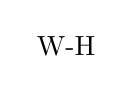
\begin{tikzpicture}

\begin{axis}[%
width=0.95092\figurewidth,
height=\figureheight,
at={(0\figurewidth,0\figureheight)},
scale only axis,
every outer x axis line/.append style={black},
every x tick label/.append style={font=\color{black}},
xtick={0,0.1},
xmin=0,
xmax=0.1,
xlabel={Frequency f/fs},
every outer y axis line/.append style={black},
every y tick label/.append style={font=\color{black}},
ymin=-70,
ymax=20,
title={W-H},
axis x line*=bottom,
axis y line*=left
]
\addplot [color=black,solid,forget plot]
  table[row sep=crcr]{%
0.000244140625	11.8967673623951\\
0.00048828125	11.9461970794956\\
0.000732421875	11.9109400314314\\
0.0009765625	11.9899704340962\\
0.001220703125	11.9641879413097\\
0.00146484375	11.975174899293\\
0.001708984375	11.9879684836488\\
0.001953125	12.0027309138707\\
0.002197265625	11.8927551225188\\
0.00244140625	11.9840275751726\\
0.002685546875	11.9119362208253\\
0.0029296875	11.98279928547\\
0.003173828125	11.8474264342537\\
0.00341796875	11.9713901746289\\
0.003662109375	11.9401750931528\\
0.00390625	11.8502489151233\\
0.004150390625	11.9250031297572\\
0.00439453125	11.8111500921863\\
0.004638671875	11.8777366016921\\
0.0048828125	11.8481720026577\\
0.005126953125	11.7151153870007\\
0.00537109375	11.9034773821419\\
0.005615234375	11.7491084813392\\
0.005859375	11.8494561707548\\
0.006103515625	11.9118715586623\\
0.00634765625	11.8022932851925\\
0.006591796875	11.7684930817235\\
0.0068359375	11.8030294177545\\
0.007080078125	11.7642211244117\\
0.00732421875	11.6452802629357\\
0.007568359375	11.7339238073401\\
0.0078125	11.7545729869236\\
0.008056640625	11.7432627159873\\
0.00830078125	11.6598991539054\\
0.008544921875	11.6893783816333\\
0.0087890625	11.798912787872\\
0.009033203125	11.6588229014871\\
0.00927734375	11.654511905707\\
0.009521484375	11.6124199118888\\
0.009765625	11.5689058058296\\
0.010009765625	11.4995253171451\\
0.01025390625	11.6495657008593\\
0.010498046875	11.5420976516015\\
0.0107421875	11.5120541591511\\
0.010986328125	11.5094508915556\\
0.01123046875	11.5522988522447\\
0.011474609375	11.4878059983628\\
0.01171875	11.3640227807729\\
0.011962890625	11.454588243027\\
0.01220703125	11.4318068592941\\
0.012451171875	11.5392855053971\\
0.0126953125	11.459452281474\\
0.012939453125	11.4307279184538\\
0.01318359375	11.4138723590599\\
0.013427734375	11.2816031869457\\
0.013671875	11.3461664750844\\
0.013916015625	11.3456766002286\\
0.01416015625	11.2889704727424\\
0.014404296875	11.3042944641746\\
0.0146484375	11.2751854741115\\
0.014892578125	11.3530076964502\\
0.01513671875	11.3739427269121\\
0.015380859375	11.1270194427665\\
0.015625	11.2561911238761\\
0.015869140625	11.0754933372789\\
0.01611328125	11.2711142256783\\
0.016357421875	11.0916739657849\\
0.0166015625	11.2228028988069\\
0.016845703125	11.1510281813323\\
0.01708984375	10.962789564049\\
0.017333984375	11.109423823249\\
0.017578125	11.1022308687647\\
0.017822265625	11.0325827610728\\
0.01806640625	10.9566826534437\\
0.018310546875	11.0363870215108\\
0.0185546875	11.1760470921088\\
0.018798828125	10.9292833609753\\
0.01904296875	10.9222608521813\\
0.019287109375	11.0906824680104\\
0.01953125	10.8794695283946\\
0.019775390625	11.0479921728057\\
0.02001953125	10.9366969392211\\
0.020263671875	10.9417689153969\\
0.0205078125	10.916126206332\\
0.020751953125	10.8500008017625\\
0.02099609375	10.9011136169206\\
0.021240234375	10.9548573454983\\
0.021484375	10.8302390779762\\
0.021728515625	10.9438267777942\\
0.02197265625	10.9425684270734\\
0.022216796875	10.8509164404979\\
0.0224609375	10.8781615229768\\
0.022705078125	10.9773870965202\\
0.02294921875	10.9314351732688\\
0.023193359375	10.9626986677973\\
0.0234375	10.8315165507452\\
0.023681640625	10.8928345222742\\
0.02392578125	10.8151738133106\\
0.024169921875	10.7381451056665\\
0.0244140625	10.8011858760136\\
0.024658203125	10.8591886058924\\
0.02490234375	10.8697248435891\\
0.025146484375	10.7370128988359\\
0.025390625	10.6736234749205\\
0.025634765625	10.8149386530881\\
0.02587890625	10.8041393881481\\
0.026123046875	10.7756785743406\\
0.0263671875	10.7093436165761\\
0.026611328125	10.8061259897503\\
0.02685546875	10.7732959348025\\
0.027099609375	10.8616780960849\\
0.02734375	10.7951794011655\\
0.027587890625	10.7758715175829\\
0.02783203125	10.8716590530415\\
0.028076171875	10.9245081172693\\
0.0283203125	10.8734172206113\\
0.028564453125	10.7737396279495\\
0.02880859375	10.7740569536602\\
0.029052734375	10.8373378793347\\
0.029296875	10.8404240536425\\
0.029541015625	10.7661003623268\\
0.02978515625	10.8510517213624\\
0.030029296875	10.8260666408167\\
0.0302734375	10.8494777684235\\
0.030517578125	10.8107092348204\\
0.03076171875	10.8246969300857\\
0.031005859375	10.9778779374677\\
0.03125	10.9441743750944\\
0.031494140625	10.942993407025\\
0.03173828125	11.0302472771694\\
0.031982421875	10.9406252776228\\
0.0322265625	10.9008943134378\\
0.032470703125	10.9622895250565\\
0.03271484375	10.9927156720959\\
0.032958984375	11.1559413068186\\
0.033203125	10.9300605822337\\
0.033447265625	11.0440726060792\\
0.03369140625	10.8683180769843\\
0.033935546875	10.964972487597\\
0.0341796875	11.1078652055571\\
0.034423828125	11.1133655997153\\
0.03466796875	11.0257513830983\\
0.034912109375	11.0460252220323\\
0.03515625	11.168202606684\\
0.035400390625	11.0692259299478\\
0.03564453125	11.1819521168939\\
0.035888671875	11.2339944206053\\
0.0361328125	11.1369212222397\\
0.036376953125	11.2357322260212\\
0.03662109375	11.2512726726085\\
0.036865234375	11.2486433517956\\
0.037109375	11.2441317564784\\
0.037353515625	11.2533314209157\\
0.03759765625	11.2752946141053\\
0.037841796875	11.3600051764651\\
0.0380859375	11.3209219839002\\
0.038330078125	11.4148012256632\\
0.03857421875	11.2803411056506\\
0.038818359375	11.3009137784343\\
0.0390625	11.4475595073291\\
0.039306640625	11.3237728001062\\
0.03955078125	11.2898680125511\\
0.039794921875	11.3227145211979\\
0.0400390625	11.4869002960432\\
0.040283203125	11.4232122593625\\
0.04052734375	11.4337443532263\\
0.040771484375	11.4787389231116\\
0.041015625	11.4752652836864\\
0.041259765625	11.5359886728405\\
0.04150390625	11.5227826828053\\
0.041748046875	11.5505735406571\\
0.0419921875	11.4719132933298\\
0.042236328125	11.5241089174805\\
0.04248046875	11.4400539352363\\
0.042724609375	11.5867936119404\\
0.04296875	11.5000352452\\
0.043212890625	11.4529973598893\\
0.04345703125	11.555386666006\\
0.043701171875	11.5548506615763\\
0.0439453125	11.5020480898589\\
0.044189453125	11.4851667298369\\
0.04443359375	11.3923721371974\\
0.044677734375	11.4582902736834\\
0.044921875	11.4305084860237\\
0.045166015625	11.3003844989548\\
0.04541015625	11.3996397099041\\
0.045654296875	11.3927921033565\\
0.0458984375	11.3747109102515\\
0.046142578125	11.3343742627104\\
0.04638671875	11.2551140959841\\
0.046630859375	11.1516612708439\\
0.046875	11.2067493556906\\
0.047119140625	11.1760479397363\\
0.04736328125	11.1704283361356\\
0.047607421875	10.9950060497436\\
0.0478515625	10.9239329279278\\
0.048095703125	10.9033612100858\\
0.04833984375	10.9623597819265\\
0.048583984375	10.8460212599238\\
0.048828125	10.7964132979894\\
0.049072265625	10.7537378739859\\
0.04931640625	10.5825132458122\\
0.049560546875	10.4304030460294\\
0.0498046875	10.4708916782022\\
0.050048828125	10.3427319484714\\
0.05029296875	10.2463134420859\\
0.050537109375	10.1564371355034\\
0.05078125	10.0685482718835\\
0.051025390625	10.0417975933067\\
0.05126953125	9.92840100869262\\
0.051513671875	9.76616432730003\\
0.0517578125	9.69056050812191\\
0.052001953125	9.60175590218711\\
0.05224609375	9.5329920390779\\
0.052490234375	9.33983437651654\\
0.052734375	9.3292888851426\\
0.052978515625	9.13449661550993\\
0.05322265625	8.98764031407143\\
0.053466796875	8.9027295425671\\
0.0537109375	8.77631645335885\\
0.053955078125	8.77449151010262\\
0.05419921875	8.61458830390461\\
0.054443359375	8.32866499924171\\
0.0546875	8.19699941391269\\
0.054931640625	8.11618199747107\\
0.05517578125	8.06597729452653\\
0.055419921875	7.82808089022427\\
0.0556640625	7.61587866401976\\
0.055908203125	7.57517724139029\\
0.05615234375	7.42430330821082\\
0.056396484375	7.31298768100493\\
0.056640625	7.04494167404863\\
0.056884765625	6.95919499788579\\
0.05712890625	6.88985803582835\\
0.057373046875	6.70848093985893\\
0.0576171875	6.75176439049972\\
0.057861328125	6.51296290389706\\
0.05810546875	6.31342503884912\\
0.058349609375	6.18223213390024\\
0.05859375	5.99709543524483\\
0.058837890625	5.94026347297654\\
0.05908203125	5.76213438532119\\
0.059326171875	5.51075565142247\\
0.0595703125	5.3689155955027\\
0.059814453125	5.32230886438316\\
0.06005859375	5.16862913357704\\
0.060302734375	5.03469458233945\\
0.060546875	4.89333339049932\\
0.060791015625	4.7957401431317\\
0.06103515625	4.63509771429847\\
0.061279296875	4.42705333519962\\
0.0615234375	4.25820374993845\\
0.061767578125	4.17846528880625\\
0.06201171875	3.93992434827533\\
0.062255859375	3.94461741466336\\
0.0625	3.73972990958021\\
0.062744140625	3.61285401955746\\
0.06298828125	3.44976701522637\\
0.063232421875	3.26777132789152\\
0.0634765625	3.06229069310871\\
0.063720703125	2.98525209498615\\
0.06396484375	2.92157099121584\\
0.064208984375	2.76405986084455\\
0.064453125	2.6837717813687\\
0.064697265625	2.38964853434788\\
0.06494140625	2.27819540199954\\
0.065185546875	2.07087077772707\\
0.0654296875	1.97344896423414\\
0.065673828125	1.72965329287064\\
0.06591796875	1.78718506435871\\
0.066162109375	1.59190482100075\\
0.06640625	1.5906731668112\\
0.066650390625	1.2993633647435\\
0.06689453125	1.15718652908168\\
0.067138671875	1.09006931343379\\
0.0673828125	0.991389743773254\\
0.067626953125	0.805498067262874\\
0.06787109375	0.709585063220516\\
0.068115234375	0.579802814040761\\
0.068359375	0.501271556144843\\
0.068603515625	0.137727997596414\\
0.06884765625	0.0698208905877777\\
0.069091796875	0.0198012001828261\\
0.0693359375	-0.11719573804703\\
0.069580078125	-0.442427963042405\\
0.06982421875	-0.403630853588879\\
0.070068359375	-0.600219197747322\\
0.0703125	-0.705446611192428\\
0.070556640625	-0.824825791774174\\
0.07080078125	-0.906503037357083\\
0.071044921875	-1.07962650312152\\
0.0712890625	-1.13182038248874\\
0.071533203125	-1.27021560634785\\
0.07177734375	-1.47720773237666\\
0.072021484375	-1.61094509592527\\
0.072265625	-1.61478861227346\\
0.072509765625	-1.84433537272042\\
0.07275390625	-1.92491749817344\\
0.072998046875	-1.97116162735819\\
0.0732421875	-2.25135789370523\\
0.073486328125	-2.4379328539074\\
0.07373046875	-2.49776247292669\\
0.073974609375	-2.60918304955533\\
0.07421875	-2.59525167379155\\
0.074462890625	-2.74418497599612\\
0.07470703125	-2.92733581254492\\
0.074951171875	-2.86581515363412\\
0.0751953125	-3.13266853239082\\
0.075439453125	-3.15845409601201\\
0.07568359375	-3.30368177995507\\
0.075927734375	-3.55696481839914\\
0.076171875	-3.59199262428825\\
0.076416015625	-3.77395123923134\\
0.07666015625	-3.96998023498668\\
0.076904296875	-3.95960386318279\\
0.0771484375	-4.09149149884604\\
0.077392578125	-4.2908120233655\\
0.07763671875	-4.26700368555856\\
0.077880859375	-4.33038160459364\\
0.078125	-4.45828737985556\\
0.078369140625	-4.59272508961516\\
0.07861328125	-4.78639182236748\\
0.078857421875	-4.79134172420015\\
0.0791015625	-4.99251500728809\\
0.079345703125	-5.01007535255752\\
0.07958984375	-5.20546299501871\\
0.079833984375	-5.35483448774175\\
0.080078125	-5.40516847915188\\
0.080322265625	-5.64698203625642\\
0.08056640625	-5.56313989407005\\
0.080810546875	-5.70737623774733\\
0.0810546875	-5.78976257105029\\
0.081298828125	-5.94342861204183\\
0.08154296875	-6.11455503500241\\
0.081787109375	-6.23255486873558\\
0.08203125	-6.36893792320978\\
0.082275390625	-6.27100132230629\\
0.08251953125	-6.47901506270409\\
0.082763671875	-6.71544031375885\\
0.0830078125	-6.68571001026788\\
0.083251953125	-6.88359590948301\\
0.08349609375	-6.85801612139505\\
0.083740234375	-6.95741197219866\\
0.083984375	-7.10045597950943\\
0.084228515625	-7.22081192728831\\
0.08447265625	-7.31164306562266\\
0.084716796875	-7.38348476678357\\
0.0849609375	-7.58832465450712\\
0.085205078125	-7.70008484264571\\
0.08544921875	-7.9359146858518\\
0.085693359375	-7.8728427398151\\
0.0859375	-8.00167174130138\\
0.086181640625	-8.11751394916661\\
0.08642578125	-8.12631668935325\\
0.086669921875	-8.17499335927789\\
0.0869140625	-8.28204938185706\\
0.087158203125	-8.39618958768864\\
0.08740234375	-8.53672214019701\\
0.087646484375	-8.6926250575508\\
0.087890625	-8.74437440815194\\
0.088134765625	-8.71953630723931\\
0.08837890625	-8.95426362228943\\
0.088623046875	-8.95767476446326\\
0.0888671875	-9.20771453849494\\
0.089111328125	-9.14304877827095\\
0.08935546875	-9.30263119799451\\
0.089599609375	-9.46110795365792\\
0.08984375	-9.48404266281193\\
0.090087890625	-9.58213152840699\\
0.09033203125	-9.69503642029463\\
0.090576171875	-9.75674210195353\\
0.0908203125	-10.034081029752\\
0.091064453125	-9.98759297851387\\
0.09130859375	-10.0934944428195\\
0.091552734375	-10.239532046874\\
0.091796875	-10.3763588191916\\
0.092041015625	-10.3917049264256\\
0.09228515625	-10.4592467549293\\
0.092529296875	-10.5434789932366\\
0.0927734375	-10.6709540098997\\
0.093017578125	-10.7425020726404\\
0.09326171875	-10.8090933256947\\
0.093505859375	-10.9065707469809\\
0.09375	-10.9067949067456\\
0.093994140625	-11.0087203679117\\
0.09423828125	-11.1446824429572\\
0.094482421875	-11.3349554996053\\
0.0947265625	-11.4023589788622\\
0.094970703125	-11.5371893540749\\
0.09521484375	-11.5419145756013\\
0.095458984375	-11.6146621651778\\
0.095703125	-11.8429253579775\\
0.095947265625	-11.8303986235952\\
0.09619140625	-11.9560371578222\\
0.096435546875	-12.0898986348986\\
0.0966796875	-12.0798071403929\\
0.096923828125	-12.1832358150968\\
0.09716796875	-12.3373034861751\\
0.097412109375	-12.50162916148\\
0.09765625	-12.49407531758\\
0.097900390625	-12.4602311782955\\
0.09814453125	-12.7021320836827\\
0.098388671875	-12.7292300583144\\
0.0986328125	-12.8081960187865\\
0.098876953125	-12.8590349431216\\
0.09912109375	-13.0331466092161\\
0.099365234375	-13.1282264692277\\
0.099609375	-13.2403487982526\\
0.099853515625	-13.1331636015722\\
};
\addplot [color=blue,solid,forget plot]
  table[row sep=crcr]{%
0.000244140625	-17.6365716382082\\
0.00048828125	-16.4964699298994\\
0.000732421875	-19.7113823288877\\
0.0009765625	-18.5009893823567\\
0.001220703125	-18.1393673665044\\
0.00146484375	-19.4049463302477\\
0.001708984375	-17.4500591579966\\
0.001953125	-17.8248801593517\\
0.002197265625	-17.9621607424444\\
0.00244140625	-17.1961390584435\\
0.002685546875	-15.6998507395566\\
0.0029296875	-19.1229774377889\\
0.003173828125	-19.2737093591144\\
0.00341796875	-19.1514845954975\\
0.003662109375	-17.7258067475125\\
0.00390625	-21.5026723646887\\
0.004150390625	-18.3141242361821\\
0.00439453125	-18.166565840876\\
0.004638671875	-15.6239626363626\\
0.0048828125	-20.6207820031885\\
0.005126953125	-21.4500430914475\\
0.00537109375	-19.7874817580728\\
0.005615234375	-19.4124128666638\\
0.005859375	-17.4319289265802\\
0.006103515625	-16.4798613153141\\
0.00634765625	-16.340150725841\\
0.006591796875	-18.714046681117\\
0.0068359375	-18.1983035165082\\
0.007080078125	-16.9683845458072\\
0.00732421875	-16.7718928424292\\
0.007568359375	-15.7301927626432\\
0.0078125	-18.9564409143126\\
0.008056640625	-19.3804383948045\\
0.00830078125	-19.5410396846357\\
0.008544921875	-18.1476042235116\\
0.0087890625	-18.7943911073962\\
0.009033203125	-18.498531819803\\
0.00927734375	-17.1637938125918\\
0.009521484375	-17.7369932296658\\
0.009765625	-21.2408731412089\\
0.010009765625	-20.1763986705263\\
0.01025390625	-19.6725331182952\\
0.010498046875	-16.19979574318\\
0.0107421875	-23.9022196571688\\
0.010986328125	-17.0837115903685\\
0.01123046875	-17.987617647594\\
0.011474609375	-18.1736923491521\\
0.01171875	-17.0488013546019\\
0.011962890625	-18.4737826731291\\
0.01220703125	-18.5860672573737\\
0.012451171875	-19.0114592962811\\
0.0126953125	-16.9667076796624\\
0.012939453125	-16.8229656431505\\
0.01318359375	-19.8814721657172\\
0.013427734375	-19.5806100298412\\
0.013671875	-18.6952027072421\\
0.013916015625	-18.7912097492374\\
0.01416015625	-20.8517188211848\\
0.014404296875	-17.3525804601253\\
0.0146484375	-20.7500491951423\\
0.014892578125	-19.3081288581438\\
0.01513671875	-17.4958974482598\\
0.015380859375	-18.3577609966547\\
0.015625	-17.2409275542159\\
0.015869140625	-20.4307388817366\\
0.01611328125	-19.9083109065506\\
0.016357421875	-16.9388910794553\\
0.0166015625	-19.2015569731469\\
0.016845703125	-20.8963230979374\\
0.01708984375	-19.1836914901409\\
0.017333984375	-20.3512549939121\\
0.017578125	-17.7326755534794\\
0.017822265625	-19.9267983482068\\
0.01806640625	-20.5823902317377\\
0.018310546875	-19.0790297499913\\
0.0185546875	-17.7773759960341\\
0.018798828125	-20.4415805217155\\
0.01904296875	-17.8808209157539\\
0.019287109375	-17.2275333234631\\
0.01953125	-19.9823780091564\\
0.019775390625	-16.9298966194971\\
0.02001953125	-20.8287575668963\\
0.020263671875	-17.6423031453159\\
0.0205078125	-19.0498427585302\\
0.020751953125	-17.8580862523335\\
0.02099609375	-19.488818137018\\
0.021240234375	-19.9295715030554\\
0.021484375	-18.3416678131839\\
0.021728515625	-18.2383863962279\\
0.02197265625	-18.8194062448532\\
0.022216796875	-22.7867098923685\\
0.0224609375	-19.18120178853\\
0.022705078125	-19.3294776503985\\
0.02294921875	-18.7740713596047\\
0.023193359375	-19.3952430168385\\
0.0234375	-17.6557105215425\\
0.023681640625	-20.5518052523167\\
0.02392578125	-22.2593269981135\\
0.024169921875	-17.8620239092422\\
0.0244140625	-20.5498976568982\\
0.024658203125	-20.4085783397933\\
0.02490234375	-17.8912965692965\\
0.025146484375	-19.5725953101572\\
0.025390625	-18.5826559223465\\
0.025634765625	-20.4209070917257\\
0.02587890625	-19.1640995733607\\
0.026123046875	-16.3636414747486\\
0.0263671875	-18.921525453384\\
0.026611328125	-18.4736401491181\\
0.02685546875	-18.7489266461797\\
0.027099609375	-18.7496264305891\\
0.02734375	-19.3289877448955\\
0.027587890625	-19.3343870862327\\
0.02783203125	-16.3390452780145\\
0.028076171875	-18.1379420589707\\
0.0283203125	-20.7840970111237\\
0.028564453125	-18.2828612602402\\
0.02880859375	-19.1910708460632\\
0.029052734375	-20.6620455832003\\
0.029296875	-20.2072626627983\\
0.029541015625	-19.7834615258303\\
0.02978515625	-17.3533552551817\\
0.030029296875	-18.6577390351239\\
0.0302734375	-17.8257393469001\\
0.030517578125	-19.969282319967\\
0.03076171875	-17.5015805079251\\
0.031005859375	-17.7249776443931\\
0.03125	-17.3453412153616\\
0.031494140625	-17.9678639741111\\
0.03173828125	-17.6456832260442\\
0.031982421875	-20.7949439226397\\
0.0322265625	-18.6903639712571\\
0.032470703125	-20.2420150529053\\
0.03271484375	-16.9666033783154\\
0.032958984375	-20.3558652117213\\
0.033203125	-19.7877972346399\\
0.033447265625	-19.4080869106753\\
0.03369140625	-18.3645072255021\\
0.033935546875	-19.1321367703922\\
0.0341796875	-18.3161609838968\\
0.034423828125	-21.268982006902\\
0.03466796875	-17.7387516292915\\
0.034912109375	-18.2548487199591\\
0.03515625	-18.342715947921\\
0.035400390625	-20.5723777200267\\
0.03564453125	-17.604233804999\\
0.035888671875	-18.6071578903593\\
0.0361328125	-17.3075178609836\\
0.036376953125	-18.0365654666252\\
0.03662109375	-18.5459129685691\\
0.036865234375	-17.9696164197366\\
0.037109375	-19.4796599904219\\
0.037353515625	-20.495204868123\\
0.03759765625	-16.3808695637358\\
0.037841796875	-18.8817392405836\\
0.0380859375	-14.9894506054156\\
0.038330078125	-18.583991391175\\
0.03857421875	-20.4765139839677\\
0.038818359375	-19.8731486734571\\
0.0390625	-21.6580423798511\\
0.039306640625	-18.9888448459643\\
0.03955078125	-17.892764976873\\
0.039794921875	-20.2664278439999\\
0.0400390625	-17.6360391196574\\
0.040283203125	-15.3867452050238\\
0.04052734375	-18.4635090061629\\
0.040771484375	-21.3136268792449\\
0.041015625	-15.2411642084844\\
0.041259765625	-18.831151221542\\
0.04150390625	-19.5149225421155\\
0.041748046875	-21.2187807809164\\
0.0419921875	-18.0017326287098\\
0.042236328125	-18.1526672802692\\
0.04248046875	-16.3493404625617\\
0.042724609375	-17.0207025736826\\
0.04296875	-17.6445501585895\\
0.043212890625	-16.0138401239372\\
0.04345703125	-15.0742913802498\\
0.043701171875	-23.8538864426792\\
0.0439453125	-17.7317881816124\\
0.044189453125	-21.6111082647586\\
0.04443359375	-16.0484901293606\\
0.044677734375	-17.4880725010738\\
0.044921875	-17.7251831222428\\
0.045166015625	-17.5995736822345\\
0.04541015625	-16.0608119454639\\
0.045654296875	-21.5654951118223\\
0.0458984375	-20.0185309331114\\
0.046142578125	-18.5508943506772\\
0.04638671875	-17.6407540383162\\
0.046630859375	-20.0524669659105\\
0.046875	-19.4402778511773\\
0.047119140625	-18.2634967525593\\
0.04736328125	-18.8794972256492\\
0.047607421875	-20.4545681913564\\
0.0478515625	-19.121025174183\\
0.048095703125	-18.3417750798691\\
0.04833984375	-19.1486072125364\\
0.048583984375	-18.1412842249754\\
0.048828125	-19.5373615440381\\
0.049072265625	-17.8007347653852\\
0.04931640625	-17.9109548870841\\
0.049560546875	-20.6388815811789\\
0.0498046875	-18.4861559165583\\
0.050048828125	-20.4940476887739\\
0.05029296875	-19.4547918702245\\
0.050537109375	-17.7549645428707\\
0.05078125	-20.3548934069639\\
0.051025390625	-21.379732576457\\
0.05126953125	-19.9813672261147\\
0.051513671875	-19.3121575984323\\
0.0517578125	-18.5195320956469\\
0.052001953125	-19.5206859493829\\
0.05224609375	-20.3190462474924\\
0.052490234375	-19.2703062949382\\
0.052734375	-19.07256853678\\
0.052978515625	-21.9755842639208\\
0.05322265625	-20.9989435358838\\
0.053466796875	-18.2381558004087\\
0.0537109375	-22.707886896842\\
0.053955078125	-21.9181573481106\\
0.05419921875	-21.9625211668284\\
0.054443359375	-20.1379912935683\\
0.0546875	-21.5148959472906\\
0.054931640625	-21.5618438129356\\
0.05517578125	-21.0822574950495\\
0.055419921875	-21.2128754175112\\
0.0556640625	-22.3937422173107\\
0.055908203125	-24.2393594028983\\
0.05615234375	-23.6721926660506\\
0.056396484375	-23.8512822351083\\
0.056640625	-23.1847962503511\\
0.056884765625	-22.3073790675155\\
0.05712890625	-25.9527389323503\\
0.057373046875	-22.0190778556306\\
0.0576171875	-24.4278379372462\\
0.057861328125	-24.9863416157393\\
0.05810546875	-24.1288261027448\\
0.058349609375	-25.7151359389262\\
0.05859375	-23.0215286313984\\
0.058837890625	-27.0402235807479\\
0.05908203125	-20.9536737681394\\
0.059326171875	-24.9363331347942\\
0.0595703125	-22.6106382517224\\
0.059814453125	-24.4382777585813\\
0.06005859375	-23.2087413504102\\
0.060302734375	-23.8027262450771\\
0.060546875	-24.1662022963062\\
0.060791015625	-26.0653045645811\\
0.06103515625	-28.4287119242304\\
0.061279296875	-26.8799957464897\\
0.0615234375	-25.2385106276179\\
0.061767578125	-25.0160707014874\\
0.06201171875	-27.9781105693597\\
0.062255859375	-26.1220197091457\\
0.0625	-25.9805931582835\\
0.062744140625	-24.8354915368235\\
0.06298828125	-24.5251634029205\\
0.063232421875	-27.2238515033813\\
0.0634765625	-29.076183970767\\
0.063720703125	-24.3826603678837\\
0.06396484375	-26.2110940975682\\
0.064208984375	-28.4000800706092\\
0.064453125	-27.1459058245503\\
0.064697265625	-27.5080361445322\\
0.06494140625	-28.7929579465362\\
0.065185546875	-26.6171653017992\\
0.0654296875	-28.1552282741588\\
0.065673828125	-29.6362673212044\\
0.06591796875	-29.7097289904723\\
0.066162109375	-30.6781426485869\\
0.06640625	-29.3357664596348\\
0.066650390625	-27.6644871920437\\
0.06689453125	-30.0047613224723\\
0.067138671875	-26.8298088129437\\
0.0673828125	-29.3085575752867\\
0.067626953125	-29.898564894228\\
0.06787109375	-28.3232455638905\\
0.068115234375	-29.5293281338082\\
0.068359375	-29.7704094473207\\
0.068603515625	-29.7102302472797\\
0.06884765625	-29.6532769454839\\
0.069091796875	-28.1795167787583\\
0.0693359375	-31.2215253151158\\
0.069580078125	-30.2357312561456\\
0.06982421875	-31.7636212966287\\
0.070068359375	-29.9246202880182\\
0.0703125	-29.9399371377565\\
0.070556640625	-29.8818460072591\\
0.07080078125	-34.1151746811245\\
0.071044921875	-28.031170866219\\
0.0712890625	-30.2695934259722\\
0.071533203125	-30.9899900291292\\
0.07177734375	-32.3123654711743\\
0.072021484375	-32.6816418839909\\
0.072265625	-35.3990665156123\\
0.072509765625	-31.0583359430448\\
0.07275390625	-32.7709915421656\\
0.072998046875	-34.4320491056943\\
0.0732421875	-30.0269327694797\\
0.073486328125	-32.9520714743744\\
0.07373046875	-32.4189883142761\\
0.073974609375	-33.5268141212857\\
0.07421875	-32.4353770095738\\
0.074462890625	-32.9206291595958\\
0.07470703125	-33.6478894943025\\
0.074951171875	-31.9923499034273\\
0.0751953125	-33.3887418397538\\
0.075439453125	-32.1254844269067\\
0.07568359375	-37.154442017399\\
0.075927734375	-31.129442936525\\
0.076171875	-35.040728138408\\
0.076416015625	-34.298303471384\\
0.07666015625	-32.697278067518\\
0.076904296875	-34.3476886460585\\
0.0771484375	-33.2910372695228\\
0.077392578125	-35.9726117826463\\
0.07763671875	-34.1349116413018\\
0.077880859375	-33.7243707392491\\
0.078125	-35.441500301587\\
0.078369140625	-39.0221433953806\\
0.07861328125	-34.5128116609131\\
0.078857421875	-35.3537327390903\\
0.0791015625	-34.3823777847595\\
0.079345703125	-33.2624761931374\\
0.07958984375	-33.316866403732\\
0.079833984375	-31.4370644808667\\
0.080078125	-35.1846244799555\\
0.080322265625	-34.0522367916107\\
0.08056640625	-34.6316194296058\\
0.080810546875	-33.0895072846846\\
0.0810546875	-35.4236436948639\\
0.081298828125	-35.5100892195152\\
0.08154296875	-35.6168820491616\\
0.081787109375	-35.4922631456749\\
0.08203125	-36.3821026152475\\
0.082275390625	-35.2943668257632\\
0.08251953125	-42.537197206316\\
0.082763671875	-39.6059609356823\\
0.0830078125	-35.8969443771483\\
0.083251953125	-35.5589750273055\\
0.08349609375	-34.2129855253158\\
0.083740234375	-37.2270523579286\\
0.083984375	-38.6879598088185\\
0.084228515625	-36.6824826655309\\
0.08447265625	-36.8097410488649\\
0.084716796875	-37.8122507668201\\
0.0849609375	-37.9011584219837\\
0.085205078125	-36.8352410893925\\
0.08544921875	-40.532807581621\\
0.085693359375	-39.1023587234439\\
0.0859375	-39.4754462541234\\
0.086181640625	-41.0578927133181\\
0.08642578125	-36.9786514825182\\
0.086669921875	-40.4132980141117\\
0.0869140625	-38.6942163768186\\
0.087158203125	-38.9153639047772\\
0.08740234375	-40.9079982769356\\
0.087646484375	-38.3288514572651\\
0.087890625	-41.6477938209331\\
0.088134765625	-39.738373983191\\
0.08837890625	-38.032510315328\\
0.088623046875	-38.988254886046\\
0.0888671875	-38.8644098734812\\
0.089111328125	-39.0701366154794\\
0.08935546875	-37.7707323087834\\
0.089599609375	-41.0069262306101\\
0.08984375	-38.9453847842399\\
0.090087890625	-39.7704977653305\\
0.09033203125	-37.7429320905348\\
0.090576171875	-41.2459310367626\\
0.0908203125	-42.4710712016266\\
0.091064453125	-39.4578395952877\\
0.09130859375	-43.3137226384515\\
0.091552734375	-39.358707884549\\
0.091796875	-40.6646949583492\\
0.092041015625	-41.0573868208628\\
0.09228515625	-41.1323803734948\\
0.092529296875	-43.6648296138408\\
0.0927734375	-40.442318878709\\
0.093017578125	-39.3164061434771\\
0.09326171875	-42.6992979950288\\
0.093505859375	-38.9601893504883\\
0.09375	-41.3416092090623\\
0.093994140625	-44.3088984956924\\
0.09423828125	-41.1677289893942\\
0.094482421875	-44.5308170966815\\
0.0947265625	-42.2990400522982\\
0.094970703125	-40.4336686385705\\
0.09521484375	-40.2552129635806\\
0.095458984375	-42.6469727021351\\
0.095703125	-43.3344186878376\\
0.095947265625	-40.8351599172753\\
0.09619140625	-45.8762593704107\\
0.096435546875	-41.4443448647642\\
0.0966796875	-40.1140168732019\\
0.096923828125	-44.1285646894302\\
0.09716796875	-41.845526041855\\
0.097412109375	-41.5840748814264\\
0.09765625	-41.8347687567364\\
0.097900390625	-43.3334904071249\\
0.09814453125	-42.0399579513814\\
0.098388671875	-42.3804047625206\\
0.0986328125	-41.3131229697345\\
0.098876953125	-44.0960053454132\\
0.09912109375	-40.5552067062004\\
0.099365234375	-44.346989364744\\
0.099609375	-43.4872275751175\\
0.099853515625	-43.7027226504539\\
};
\addplot [color=red,solid,forget plot]
  table[row sep=crcr]{%
0.000244140625	-27.6344005786918\\
0.00048828125	-26.4937258522904\\
0.000732421875	-29.7069786828409\\
0.0009765625	-28.4970072899564\\
0.001220703125	-28.1376531870998\\
0.00146484375	-29.4022175254802\\
0.001708984375	-27.4477474519239\\
0.001953125	-27.8215420329391\\
0.002197265625	-27.9591008058184\\
0.00244140625	-27.1943373960682\\
0.002685546875	-25.69895207656\\
0.0029296875	-29.1194466707045\\
0.003173828125	-29.2705818364594\\
0.00341796875	-29.1486351607889\\
0.003662109375	-27.72323042604\\
0.00390625	-31.4954828237384\\
0.004150390625	-28.3111033227185\\
0.00439453125	-28.1638501122497\\
0.004638671875	-25.622505828161\\
0.0048828125	-30.6159151800362\\
0.005126953125	-31.4451369663545\\
0.00537109375	-29.7834047731789\\
0.005615234375	-29.4060253552774\\
0.005859375	-27.429835765249\\
0.006103515625	-26.4773859698578\\
0.00634765625	-26.3387162534515\\
0.006591796875	-28.7131831623529\\
0.0068359375	-28.1950376445282\\
0.007080078125	-26.9663496626976\\
0.00732421875	-26.7679616559107\\
0.007568359375	-25.7289712719627\\
0.0078125	-28.9540441415727\\
0.008056640625	-29.3765838928769\\
0.00830078125	-29.5385122126412\\
0.008544921875	-28.1440456009777\\
0.0087890625	-28.7913689347731\\
0.009033203125	-28.495080553448\\
0.00927734375	-27.1621730180082\\
0.009521484375	-27.7339219387242\\
0.009765625	-31.2368050828844\\
0.010009765625	-30.1715371196417\\
0.01025390625	-29.6696344609946\\
0.010498046875	-26.1976462527269\\
0.0107421875	-33.8946700334428\\
0.010986328125	-27.0819351022222\\
0.01123046875	-27.9845264920565\\
0.011474609375	-28.171499721247\\
0.01171875	-27.0467507169419\\
0.011962890625	-28.4703672681621\\
0.01220703125	-28.5823630650852\\
0.012451171875	-29.0067261447286\\
0.0126953125	-26.9645649041787\\
0.012939453125	-26.820530497178\\
0.01318359375	-29.876369944131\\
0.013427734375	-29.5767105317803\\
0.013671875	-28.6929192121477\\
0.013916015625	-28.787923099297\\
0.01416015625	-30.8445317684814\\
0.014404296875	-27.3498954287494\\
0.0146484375	-30.746718979914\\
0.014892578125	-29.3062895250358\\
0.01513671875	-27.494774974979\\
0.015380859375	-28.3542574278486\\
0.015625	-27.2388159662081\\
0.015869140625	-30.4232205626614\\
0.01611328125	-29.9053635136921\\
0.016357421875	-26.9379840940579\\
0.0166015625	-29.199102477566\\
0.016845703125	-30.8919772097642\\
0.01708984375	-29.1813345745126\\
0.017333984375	-30.345538498331\\
0.017578125	-27.7294421800266\\
0.017822265625	-29.92153853238\\
0.01806640625	-30.5741281740956\\
0.018310546875	-29.0746640546583\\
0.0185546875	-27.7749054249127\\
0.018798828125	-30.4357566587265\\
0.01904296875	-27.8782808977488\\
0.019287109375	-27.2257830104733\\
0.01953125	-29.9779794012424\\
0.019775390625	-26.9273072345683\\
0.02001953125	-30.8252678122761\\
0.020263671875	-27.639930220346\\
0.0205078125	-29.0471747049754\\
0.020751953125	-27.8556749177723\\
0.02099609375	-29.4849013782202\\
0.021240234375	-29.9258819920198\\
0.021484375	-28.3404908388492\\
0.021728515625	-28.2350899394535\\
0.02197265625	-28.8158630862895\\
0.022216796875	-32.7786361272995\\
0.0224609375	-29.174164131648\\
0.022705078125	-29.3264778131921\\
0.02294921875	-28.7719445007526\\
0.023193359375	-29.3911491713334\\
0.0234375	-27.6522513077832\\
0.023681640625	-30.5490972091134\\
0.02392578125	-32.2560536409933\\
0.024169921875	-27.8604095152341\\
0.0244140625	-30.5438546530732\\
0.024658203125	-30.4041917363986\\
0.02490234375	-27.8889644376246\\
0.025146484375	-29.5680244452702\\
0.025390625	-28.5797737989254\\
0.025634765625	-30.4154006698615\\
0.02587890625	-29.1606258983955\\
0.026123046875	-26.3622255650026\\
0.0263671875	-28.9185356945521\\
0.026611328125	-28.4700551158114\\
0.02685546875	-28.7455884724519\\
0.027099609375	-28.7442515041765\\
0.02734375	-29.3267922426953\\
0.027587890625	-29.3317608261653\\
0.02783203125	-26.3370267605657\\
0.028076171875	-28.1343118071561\\
0.0283203125	-30.7787432453022\\
0.028564453125	-28.2806627508915\\
0.02880859375	-29.1892353837156\\
0.029052734375	-30.6577493732458\\
0.029296875	-30.2030513272359\\
0.029541015625	-29.7776604238699\\
0.02978515625	-27.3511498015198\\
0.030029296875	-28.6548633022463\\
0.0302734375	-27.8232448101708\\
0.030517578125	-29.9651399147543\\
0.03076171875	-27.4991773024245\\
0.031005859375	-27.722897809766\\
0.03125	-27.3436547355749\\
0.031494140625	-27.9657526119031\\
0.03173828125	-27.6415625831958\\
0.031982421875	-30.7888071021237\\
0.0322265625	-28.6882610279362\\
0.032470703125	-30.2371287755383\\
0.03271484375	-26.9638974699307\\
0.032958984375	-30.3516104143617\\
0.033203125	-29.7836228861138\\
0.033447265625	-29.4050438700943\\
0.03369140625	-28.3629211925961\\
0.033935546875	-29.1265952546543\\
0.0341796875	-28.3141231612503\\
0.034423828125	-31.2636726084295\\
0.03466796875	-27.7367087705967\\
0.034912109375	-28.2530891522858\\
0.03515625	-28.3402365095807\\
0.035400390625	-30.5674158428942\\
0.03564453125	-27.6017514737727\\
0.035888671875	-28.6034087670982\\
0.0361328125	-27.3047073496012\\
0.036376953125	-28.0334022125236\\
0.03662109375	-28.5412231765107\\
0.036865234375	-27.9672249138718\\
0.037109375	-29.4771834175659\\
0.037353515625	-30.4901330690821\\
0.03759765625	-26.379410584853\\
0.037841796875	-28.879237049902\\
0.0380859375	-24.9879409828843\\
0.038330078125	-28.5799231936591\\
0.03857421875	-30.4721873371383\\
0.038818359375	-29.8705391755299\\
0.0390625	-31.6522790285036\\
0.039306640625	-28.9869941008071\\
0.03955078125	-27.8893083008048\\
0.039794921875	-30.2634957662343\\
0.0400390625	-27.6333711856857\\
0.040283203125	-25.385572405974\\
0.04052734375	-28.4608812917973\\
0.040771484375	-31.3053287621077\\
0.041015625	-25.2400254482956\\
0.041259765625	-28.8282624937848\\
0.04150390625	-29.5111405007519\\
0.041748046875	-31.214834080092\\
0.0419921875	-27.9968912912017\\
0.042236328125	-28.1498267338211\\
0.04248046875	-26.3471278315578\\
0.042724609375	-27.0168466623732\\
0.04296875	-27.6424099810566\\
0.043212890625	-26.0119804560437\\
0.04345703125	-25.0731837584477\\
0.043701171875	-33.8400645374029\\
0.0439453125	-27.7288629413866\\
0.044189453125	-31.6043557970669\\
0.04443359375	-26.0468853810216\\
0.044677734375	-27.4848320236949\\
0.044921875	-27.7223374630342\\
0.045166015625	-27.5966292217302\\
0.04541015625	-26.0586500933298\\
0.045654296875	-31.558708008287\\
0.0458984375	-30.0169162970149\\
0.046142578125	-28.5489507908753\\
0.04638671875	-27.6385395148061\\
0.046630859375	-30.0472469348596\\
0.046875	-29.4364208123504\\
0.047119140625	-28.2602677650995\\
0.04736328125	-28.8760212894391\\
0.047607421875	-30.4498200957784\\
0.0478515625	-29.1177317923671\\
0.048095703125	-28.3392274291102\\
0.04833984375	-29.1464348880018\\
0.048583984375	-28.1377289821407\\
0.048828125	-29.5347505265324\\
0.049072265625	-27.7983312343511\\
0.04931640625	-27.9090963332936\\
0.049560546875	-30.6340337515494\\
0.0498046875	-28.4835220497837\\
0.050048828125	-30.4891385453473\\
0.05029296875	-29.4503620802568\\
0.050537109375	-27.7515454199666\\
0.05078125	-30.349809946342\\
0.051025390625	-31.3743136586744\\
0.05126953125	-29.9768224091122\\
0.051513671875	-29.3066489417442\\
0.0517578125	-28.5174167724402\\
0.052001953125	-29.5173290877048\\
0.05224609375	-30.3166779054147\\
0.052490234375	-29.2682677726839\\
0.052734375	-29.069222063932\\
0.052978515625	-31.9660296869573\\
0.05322265625	-30.995132899835\\
0.053466796875	-28.2363420309933\\
0.0537109375	-32.7028355561021\\
0.053955078125	-31.9105119933362\\
0.05419921875	-31.9558119522659\\
0.054443359375	-30.1343408898206\\
0.0546875	-31.5105336462398\\
0.054931640625	-31.5535735117104\\
0.05517578125	-31.0790855018526\\
0.055419921875	-31.2082606243323\\
0.0556640625	-32.3841720103705\\
0.055908203125	-34.2281022527458\\
0.05615234375	-33.6611589864876\\
0.056396484375	-33.8337923227441\\
0.056640625	-33.1666627194014\\
0.056884765625	-32.3002387616954\\
0.05712890625	-35.9366224339792\\
0.057373046875	-32.0124772981478\\
0.0576171875	-34.416987628695\\
0.057861328125	-34.9731682255631\\
0.05810546875	-34.1187389305723\\
0.058349609375	-35.7084408376681\\
0.05859375	-33.0158011131921\\
0.058837890625	-37.0234820783899\\
0.05908203125	-30.9485228656059\\
0.059326171875	-34.9229906792479\\
0.0595703125	-32.6027818214268\\
0.059814453125	-34.4221049756782\\
0.06005859375	-33.2029407467505\\
0.060302734375	-33.7933307080294\\
0.060546875	-34.1539921452819\\
0.060791015625	-36.055729829336\\
0.06103515625	-38.4012928594157\\
0.061279296875	-36.8556077769568\\
0.0615234375	-35.2267906110684\\
0.061767578125	-35.0029970497656\\
0.06201171875	-37.9453488152135\\
0.062255859375	-36.1111937281504\\
0.0625	-35.9566407057424\\
0.062744140625	-34.8189956053322\\
0.06298828125	-34.5160402930592\\
0.063232421875	-37.2045822148033\\
0.0634765625	-39.0475270524975\\
0.063720703125	-34.3700402685858\\
0.06396484375	-36.1864130798943\\
0.064208984375	-38.3789894048978\\
0.064453125	-37.125203019363\\
0.064697265625	-37.4971664675716\\
0.06494140625	-38.7575527419472\\
0.065185546875	-36.5966019486607\\
0.0654296875	-38.1286382910626\\
0.065673828125	-39.5964161105902\\
0.06591796875	-39.665328400113\\
0.066162109375	-40.6131850519898\\
0.06640625	-39.2968631800391\\
0.066650390625	-37.6440067962616\\
0.06689453125	-39.9456154080199\\
0.067138671875	-36.8039155332962\\
0.0673828125	-39.2776106823113\\
0.067626953125	-39.8627158493041\\
0.06787109375	-38.287780058891\\
0.068115234375	-39.5013992966445\\
0.068359375	-39.7429772546865\\
0.068603515625	-39.6618927629282\\
0.06884765625	-39.6173231599668\\
0.069091796875	-38.1491972941823\\
0.0693359375	-41.165758925672\\
0.069580078125	-40.2040987858903\\
0.06982421875	-41.7095254290268\\
0.070068359375	-39.9041433007925\\
0.0703125	-39.9116160059278\\
0.070556640625	-39.8395840141151\\
0.07080078125	-43.9906817062752\\
0.071044921875	-37.9887823859107\\
0.0712890625	-40.2317828045859\\
0.071533203125	-40.94188983378\\
0.07177734375	-42.2318572191339\\
0.072021484375	-42.6096833277195\\
0.072265625	-45.238363001756\\
0.072509765625	-41.026807118054\\
0.07275390625	-42.7031294019141\\
0.072998046875	-44.2641922865384\\
0.0732421875	-39.9753189113749\\
0.073486328125	-42.8894735174696\\
0.07373046875	-42.3658569692587\\
0.073974609375	-43.3528687769996\\
0.07421875	-42.370426371449\\
0.074462890625	-42.8531255794463\\
0.07470703125	-43.5544835167884\\
0.074951171875	-41.9354128671616\\
0.0751953125	-43.2923809110202\\
0.075439453125	-42.013310823373\\
0.07568359375	-47.0330224277146\\
0.075927734375	-41.0876520163553\\
0.076171875	-44.8603623071765\\
0.076416015625	-44.1829117376942\\
0.07666015625	-42.6060084417882\\
0.076904296875	-44.2332684338337\\
0.0771484375	-43.2457166988032\\
0.077392578125	-45.8536251767508\\
0.07763671875	-44.0348946315279\\
0.077880859375	-43.6063346516202\\
0.078125	-45.2679101302888\\
0.078369140625	-48.8391496710635\\
0.07861328125	-44.3829288815055\\
0.078857421875	-45.1852046818602\\
0.0791015625	-44.2484487986056\\
0.079345703125	-43.1543841953962\\
0.07958984375	-43.197269594167\\
0.079833984375	-41.3636905827952\\
0.080078125	-45.0442044265626\\
0.080322265625	-43.9131604174133\\
0.08056640625	-44.5048650805141\\
0.080810546875	-42.9628593121947\\
0.0810546875	-45.2779584949453\\
0.081298828125	-45.4356941901834\\
0.08154296875	-45.5057639113089\\
0.081787109375	-45.3605890812307\\
0.08203125	-46.1899004862205\\
0.082275390625	-45.2130900599041\\
0.08251953125	-52.1767960187021\\
0.082763671875	-49.1693355469435\\
0.0830078125	-45.7746898452745\\
0.083251953125	-45.4336600738414\\
0.08349609375	-44.0707562394235\\
0.083740234375	-46.8968155490731\\
0.083984375	-48.4107126347715\\
0.084228515625	-46.4930113722776\\
0.08447265625	-46.6074857846906\\
0.084716796875	-47.6512509754816\\
0.0849609375	-47.5379277444488\\
0.085205078125	-46.6825408500331\\
0.08544921875	-50.1272592830019\\
0.085693359375	-48.821922673117\\
0.0859375	-49.0995701043654\\
0.086181640625	-50.8894767457186\\
0.08642578125	-46.6695578892666\\
0.086669921875	-49.9285499151771\\
0.0869140625	-48.1477536275443\\
0.087158203125	-48.3503490641287\\
0.08740234375	-50.3941518539305\\
0.087646484375	-48.0715363905065\\
0.087890625	-51.0549320053608\\
0.088134765625	-49.3331961209003\\
0.08837890625	-47.7259003308603\\
0.088623046875	-48.7480415279265\\
0.0888671875	-48.5935865352066\\
0.089111328125	-48.8653600731923\\
0.08935546875	-47.5720465485119\\
0.089599609375	-50.5015473663014\\
0.08984375	-48.5663019796888\\
0.090087890625	-49.2785917949396\\
0.09033203125	-47.4422313828157\\
0.090576171875	-50.7734976275581\\
0.0908203125	-51.8241562749175\\
0.091064453125	-49.2109412130011\\
0.09130859375	-52.5469313006994\\
0.091552734375	-48.9632707231257\\
0.091796875	-50.4193440047497\\
0.092041015625	-50.4217520242751\\
0.09228515625	-50.8233065882096\\
0.092529296875	-52.7955222563928\\
0.0927734375	-49.9503134589747\\
0.093017578125	-49.0028376789957\\
0.09326171875	-51.8766440112287\\
0.093505859375	-48.7672669369458\\
0.09375	-50.8571802147216\\
0.093994140625	-52.7207304606641\\
0.09423828125	-50.8626407673678\\
0.094482421875	-53.2980068036521\\
0.0947265625	-51.4684796241559\\
0.094970703125	-49.9093774963341\\
0.09521484375	-49.8580771563365\\
0.095458984375	-52.1784657418045\\
0.095703125	-51.7981926823354\\
0.095947265625	-50.5021591723333\\
0.09619140625	-54.1331613761672\\
0.096435546875	-51.0418563560977\\
0.0966796875	-49.6771418323747\\
0.096923828125	-52.6610541183832\\
0.09716796875	-51.0423298211974\\
0.097412109375	-51.1329103445192\\
0.09765625	-51.2446490345046\\
0.097900390625	-52.7105601593608\\
0.09814453125	-51.4446034219424\\
0.098388671875	-51.9979222340134\\
0.0986328125	-50.4385582123907\\
0.098876953125	-53.2495238662745\\
0.09912109375	-49.8176209060913\\
0.099365234375	-53.6421644484313\\
0.099609375	-52.5784903994288\\
0.099853515625	-52.9603486717047\\
};
\addplot [color=green,solid,forget plot]
  table[row sep=crcr]{%
0.000244140625	-60.6466118846863\\
0.00048828125	-58.4889770309633\\
0.000732421875	-59.6488993900514\\
0.0009765625	-58.8757279654189\\
0.001220703125	-62.1757906328416\\
0.00146484375	-61.4217003179457\\
0.001708984375	-60.1874202279458\\
0.001953125	-58.9660263113609\\
0.002197265625	-59.4813494776953\\
0.00244140625	-61.0163472177402\\
0.002685546875	-62.5412759184399\\
0.0029296875	-60.0203643554326\\
0.003173828125	-60.6979839739982\\
0.00341796875	-60.9803158123375\\
0.003662109375	-59.9923611042343\\
0.00390625	-59.309908594097\\
0.004150390625	-59.8890739573179\\
0.00439453125	-60.2041873169787\\
0.004638671875	-60.3670535468738\\
0.0048828125	-60.1237358233081\\
0.005126953125	-60.918046737463\\
0.00537109375	-60.0598951961171\\
0.005615234375	-57.7337449594179\\
0.005859375	-60.6006983864651\\
0.006103515625	-58.920108525548\\
0.00634765625	-61.1503546484888\\
0.006591796875	-65.7287402364301\\
0.0068359375	-59.4345220242881\\
0.007080078125	-60.2598155077686\\
0.00732421875	-57.2025337161338\\
0.007568359375	-61.2385235374231\\
0.0078125	-61.5368170206072\\
0.008056640625	-59.8966714424129\\
0.00830078125	-61.8907554791821\\
0.008544921875	-59.0108486591414\\
0.0087890625	-60.3675303751602\\
0.009033203125	-59.4948644081978\\
0.00927734375	-61.443546736145\\
0.009521484375	-59.2400910181135\\
0.009765625	-61.5228103576777\\
0.010009765625	-59.6840624236763\\
0.01025390625	-61.4269580913437\\
0.010498046875	-59.2532088610474\\
0.0107421875	-61.4970343426093\\
0.010986328125	-60.9650432893319\\
0.01123046875	-59.4627065113596\\
0.011474609375	-61.1407897323466\\
0.01171875	-60.3067298188175\\
0.011962890625	-59.5154959149959\\
0.01220703125	-59.2751229098998\\
0.012451171875	-58.635431513414\\
0.0126953125	-60.0337126729427\\
0.012939453125	-59.3343411293869\\
0.01318359375	-59.1791707599817\\
0.013427734375	-60.0464161607537\\
0.013671875	-61.4859031932345\\
0.013916015625	-59.9998749333586\\
0.01416015625	-58.6604596163484\\
0.014404296875	-59.4395873381793\\
0.0146484375	-61.901504069999\\
0.014892578125	-63.0384483897187\\
0.01513671875	-63.3714191934445\\
0.015380859375	-59.2887456977414\\
0.015625	-60.3716229614621\\
0.015869140625	-58.0436147619402\\
0.01611328125	-61.5902999708515\\
0.016357421875	-63.7402777424048\\
0.0166015625	-61.6785502352453\\
0.016845703125	-60.8912076154481\\
0.01708984375	-61.8369157307046\\
0.017333984375	-59.1549408244761\\
0.017578125	-59.0123431967812\\
0.017822265625	-59.0923059125464\\
0.01806640625	-57.7852194549924\\
0.018310546875	-59.0541555874716\\
0.0185546875	-60.2260101585603\\
0.018798828125	-59.1643998848074\\
0.01904296875	-60.2090260062883\\
0.019287109375	-61.173344091488\\
0.01953125	-59.9248691198043\\
0.019775390625	-59.1744788164926\\
0.02001953125	-61.7769067766965\\
0.020263671875	-60.2661196780988\\
0.0205078125	-61.1644063488913\\
0.020751953125	-60.4121489337064\\
0.02099609375	-59.9354344474013\\
0.021240234375	-60.6358815929627\\
0.021484375	-64.01125249949\\
0.021728515625	-59.4341073233851\\
0.02197265625	-59.7015717746516\\
0.022216796875	-60.0897544161865\\
0.0224609375	-57.0812447061929\\
0.022705078125	-60.9348438854492\\
0.02294921875	-61.873464308437\\
0.023193359375	-59.6497245553911\\
0.0234375	-58.6420499157216\\
0.023681640625	-62.6017383867132\\
0.02392578125	-63.48559943956\\
0.024169921875	-62.1589644305116\\
0.0244140625	-59.1121902262531\\
0.024658203125	-60.3629442626292\\
0.02490234375	-60.5904428944586\\
0.025146484375	-59.34816895117\\
0.025390625	-60.361932147357\\
0.025634765625	-59.3873018929801\\
0.02587890625	-60.1323139461744\\
0.026123046875	-61.2304209027515\\
0.0263671875	-60.5415120264074\\
0.026611328125	-59.3047586739359\\
0.02685546875	-59.890011217157\\
0.027099609375	-57.8210565756254\\
0.02734375	-62.2903942939527\\
0.027587890625	-61.5175397008065\\
0.02783203125	-59.6655540136518\\
0.028076171875	-58.9146024077622\\
0.0283203125	-59.8726692577848\\
0.028564453125	-61.2383219052294\\
0.02880859375	-62.9305413966569\\
0.029052734375	-60.7068854435769\\
0.029296875	-60.3388014608053\\
0.029541015625	-58.5232987778403\\
0.02978515625	-60.2951162207772\\
0.030029296875	-60.4466587759869\\
0.0302734375	-60.2324361034623\\
0.030517578125	-60.1725282698451\\
0.03076171875	-60.070312869135\\
0.031005859375	-60.9214927537797\\
0.03125	-61.4525296581376\\
0.031494140625	-61.0990239262748\\
0.03173828125	-57.8718161125028\\
0.031982421875	-59.2902840477418\\
0.0322265625	-61.8388798938969\\
0.032470703125	-59.727633639712\\
0.03271484375	-59.0199625829558\\
0.032958984375	-60.4427919417864\\
0.033203125	-59.9576659411226\\
0.033447265625	-60.9513309745548\\
0.03369140625	-62.7384353625362\\
0.033935546875	-58.0709231211729\\
0.0341796875	-61.6013213029133\\
0.034423828125	-60.3937169447599\\
0.03466796875	-61.0131899992163\\
0.034912109375	-62.1777522740532\\
0.03515625	-60.7757861573037\\
0.035400390625	-59.9912795989266\\
0.03564453125	-60.032238388301\\
0.035888671875	-59.2438291159526\\
0.0361328125	-59.1961021575931\\
0.036376953125	-59.4114860580927\\
0.03662109375	-58.2098751057979\\
0.036865234375	-60.5595492224625\\
0.037109375	-61.9177536719791\\
0.037353515625	-59.8188914625151\\
0.03759765625	-61.1174931071108\\
0.037841796875	-61.2751271742097\\
0.0380859375	-59.5778551944059\\
0.038330078125	-58.8657799437492\\
0.03857421875	-60.4906791284222\\
0.038818359375	-62.0841174100182\\
0.0390625	-60.4262525385567\\
0.039306640625	-62.6922963371889\\
0.03955078125	-58.8822928085063\\
0.039794921875	-61.971049989298\\
0.0400390625	-59.7507974264481\\
0.040283203125	-61.0717658511465\\
0.04052734375	-60.6442566422228\\
0.040771484375	-58.4975246621646\\
0.041015625	-61.054115171505\\
0.041259765625	-60.6004837456661\\
0.04150390625	-60.1136117537979\\
0.041748046875	-61.6323083301328\\
0.0419921875	-57.5275012478562\\
0.042236328125	-59.995071091013\\
0.04248046875	-59.2769872777879\\
0.042724609375	-57.5353472278987\\
0.04296875	-60.7168251326813\\
0.043212890625	-59.6963994377615\\
0.04345703125	-61.007665713934\\
0.043701171875	-58.8191376465961\\
0.0439453125	-59.4465532234558\\
0.044189453125	-59.6909495573894\\
0.04443359375	-60.3714614952527\\
0.044677734375	-58.7582053339622\\
0.044921875	-59.559774443158\\
0.045166015625	-59.2858871491531\\
0.04541015625	-59.0893142289954\\
0.045654296875	-59.6230994883226\\
0.0458984375	-64.3148201306789\\
0.046142578125	-62.0417865666698\\
0.04638671875	-60.5646868900171\\
0.046630859375	-59.2509689381902\\
0.046875	-59.9536521950011\\
0.047119140625	-59.5490616880089\\
0.04736328125	-59.8448842772785\\
0.047607421875	-60.064842514137\\
0.0478515625	-60.3208006596416\\
0.048095703125	-60.6569453742846\\
0.04833984375	-62.1561170456923\\
0.048583984375	-59.0086568972352\\
0.048828125	-61.7458012470957\\
0.049072265625	-60.3688787168258\\
0.04931640625	-61.5961173398164\\
0.049560546875	-60.1588270665776\\
0.0498046875	-60.6567439911475\\
0.050048828125	-59.9593787915431\\
0.05029296875	-59.3665885475078\\
0.050537109375	-58.7919508596798\\
0.05078125	-59.668599904515\\
0.051025390625	-60.4157403306274\\
0.05126953125	-59.7817737224123\\
0.051513671875	-58.2767890218905\\
0.0517578125	-61.6425501643289\\
0.052001953125	-60.6375160614514\\
0.05224609375	-62.9512608251475\\
0.052490234375	-62.553975537416\\
0.052734375	-60.2028652494187\\
0.052978515625	-58.5465345817572\\
0.05322265625	-61.5649064757885\\
0.053466796875	-62.0292712537506\\
0.0537109375	-62.0491374448513\\
0.053955078125	-59.4582007911102\\
0.05419921875	-60.0702924311828\\
0.054443359375	-60.890600060542\\
0.0546875	-61.4934013894187\\
0.054931640625	-58.7603378396753\\
0.05517578125	-62.4451920429709\\
0.055419921875	-60.9468885092994\\
0.0556640625	-58.9575860602192\\
0.055908203125	-60.0972881357415\\
0.05615234375	-59.6173140997941\\
0.056396484375	-57.7925011232584\\
0.056640625	-56.9687456643147\\
0.056884765625	-60.1444834079525\\
0.05712890625	-60.249814417892\\
0.057373046875	-60.1978140960267\\
0.0576171875	-60.44583388215\\
0.057861328125	-60.1606208170011\\
0.05810546875	-60.4639303171423\\
0.058349609375	-63.8320595737552\\
0.05859375	-61.8168428868623\\
0.058837890625	-61.1717489699585\\
0.05908203125	-60.2101078538924\\
0.059326171875	-60.0551456668973\\
0.0595703125	-60.0322999406041\\
0.059814453125	-58.7201844028027\\
0.06005859375	-61.9489519161915\\
0.060302734375	-60.4466546490264\\
0.060546875	-59.6707285468558\\
0.060791015625	-62.6270916908936\\
0.06103515625	-60.4123119102151\\
0.061279296875	-59.3738827304143\\
0.0615234375	-60.921210165155\\
0.061767578125	-60.2234062357458\\
0.06201171875	-59.1858910384008\\
0.062255859375	-62.1497761035658\\
0.0625	-58.5529546573294\\
0.062744140625	-59.0313156305099\\
0.06298828125	-61.2970151154041\\
0.063232421875	-60.7433996017311\\
0.0634765625	-60.867395895124\\
0.063720703125	-59.7435641826876\\
0.06396484375	-58.6529602272576\\
0.064208984375	-61.5264707017045\\
0.064453125	-60.3531014683763\\
0.064697265625	-63.5182769120836\\
0.06494140625	-59.6624153477601\\
0.065185546875	-59.8537833433096\\
0.0654296875	-60.2725889998977\\
0.065673828125	-59.9897544014854\\
0.06591796875	-59.5914654481651\\
0.066162109375	-58.8971670029169\\
0.06640625	-59.7942812680612\\
0.066650390625	-60.9187026320292\\
0.06689453125	-58.6337504079376\\
0.067138671875	-59.0628282362809\\
0.0673828125	-60.7647475235466\\
0.067626953125	-60.7136952563181\\
0.06787109375	-59.1852823746772\\
0.068115234375	-61.4326708053545\\
0.068359375	-61.7519240260334\\
0.068603515625	-59.2210417565412\\
0.06884765625	-60.4556845306401\\
0.069091796875	-59.7249731886838\\
0.0693359375	-60.1077301237655\\
0.069580078125	-61.5964174506872\\
0.06982421875	-60.7827474950412\\
0.070068359375	-63.1795602909514\\
0.0703125	-61.7825059340036\\
0.070556640625	-59.9790412356099\\
0.07080078125	-59.4791741650556\\
0.071044921875	-58.1153240332814\\
0.0712890625	-60.8523793652273\\
0.071533203125	-60.5222924455138\\
0.07177734375	-59.591488298047\\
0.072021484375	-60.4526316267182\\
0.072265625	-59.6360563716662\\
0.072509765625	-62.4333272477782\\
0.07275390625	-60.7985838776644\\
0.072998046875	-58.4763035989949\\
0.0732421875	-59.2512801595169\\
0.073486328125	-61.3329764266682\\
0.07373046875	-61.5167305693085\\
0.073974609375	-57.4132661855671\\
0.07421875	-60.6548701073245\\
0.074462890625	-60.9714086960905\\
0.07470703125	-60.2751992155299\\
0.074951171875	-60.7877448245376\\
0.0751953125	-59.879305632304\\
0.075439453125	-57.9482133005899\\
0.07568359375	-62.6285462841213\\
0.075927734375	-61.2755544963006\\
0.076171875	-58.7665335503536\\
0.076416015625	-59.9965759862911\\
0.07666015625	-59.4261437514898\\
0.076904296875	-60.0831685582752\\
0.0771484375	-63.0832466885955\\
0.077392578125	-61.5358449979345\\
0.07763671875	-60.4619116138895\\
0.077880859375	-59.3229140778616\\
0.078125	-59.337007911215\\
0.078369140625	-62.6838064154223\\
0.07861328125	-59.6900358005762\\
0.078857421875	-59.3803171947406\\
0.0791015625	-59.4243385045871\\
0.079345703125	-59.2482257766224\\
0.07958984375	-58.8575779414237\\
0.079833984375	-59.1227530721602\\
0.080078125	-60.017777055026\\
0.080322265625	-58.9278225491825\\
0.08056640625	-59.9163025297064\\
0.080810546875	-58.377890110363\\
0.0810546875	-60.0942862401695\\
0.081298828125	-63.1352425248807\\
0.08154296875	-61.4811980854889\\
0.081787109375	-60.6091004711794\\
0.08203125	-59.8259083069088\\
0.082275390625	-62.5318440385399\\
0.08251953125	-63.1657314940158\\
0.082763671875	-59.362572618569\\
0.0830078125	-61.3408671597486\\
0.083251953125	-60.8939810286957\\
0.08349609375	-58.9896296210449\\
0.083740234375	-58.2504760293261\\
0.083984375	-60.4977706182148\\
0.084228515625	-60.1898115206176\\
0.08447265625	-60.0270657292188\\
0.084716796875	-62.0410921671558\\
0.0849609375	-58.4942952491824\\
0.085205078125	-61.2981131976172\\
0.08544921875	-60.6258728855078\\
0.085693359375	-60.8608908965011\\
0.0859375	-59.9135481985007\\
0.086181640625	-65.0874230714859\\
0.08642578125	-58.3001311948526\\
0.086669921875	-59.6913517365132\\
0.0869140625	-57.420357859422\\
0.087158203125	-57.4870386391911\\
0.08740234375	-59.918051887736\\
0.087646484375	-60.472749654604\\
0.087890625	-59.9962995679908\\
0.088134765625	-59.8355961359506\\
0.08837890625	-59.3902836034094\\
0.088623046875	-61.4394661847771\\
0.0888671875	-60.7792767871545\\
0.089111328125	-62.2323870957355\\
0.08935546875	-61.0671863859453\\
0.089599609375	-60.0934590275523\\
0.08984375	-59.3449670236173\\
0.090087890625	-58.9812457041998\\
0.09033203125	-59.1882128741905\\
0.090576171875	-60.6420102946738\\
0.0908203125	-60.4129707507201\\
0.091064453125	-61.7864662438741\\
0.09130859375	-60.4557585304574\\
0.091552734375	-59.5665574855178\\
0.091796875	-63.0214075699171\\
0.092041015625	-59.0814602680351\\
0.09228515625	-62.4541484296497\\
0.092529296875	-60.2090376945329\\
0.0927734375	-59.652138223622\\
0.093017578125	-60.573197930163\\
0.09326171875	-59.5071511026285\\
0.093505859375	-62.3873873141152\\
0.09375	-60.6226853067774\\
0.093994140625	-57.859520998009\\
0.09423828125	-62.5478806004793\\
0.094482421875	-59.3687210007302\\
0.0947265625	-59.0612743060042\\
0.094970703125	-59.3510040568594\\
0.09521484375	-60.4435846620687\\
0.095458984375	-62.0812961717224\\
0.095703125	-57.0569792396041\\
0.095947265625	-61.8209867740143\\
0.09619140625	-58.9402238506195\\
0.096435546875	-61.5718547638694\\
0.0966796875	-59.8680191545354\\
0.096923828125	-58.0861980164599\\
0.09716796875	-58.7673668561638\\
0.097412109375	-61.1910334742855\\
0.09765625	-60.2048101660226\\
0.097900390625	-61.4517519226943\\
0.09814453125	-60.3689671095816\\
0.098388671875	-62.7394871355331\\
0.0986328125	-57.8284282773983\\
0.098876953125	-60.7675608189041\\
0.09912109375	-57.8809131939516\\
0.099365234375	-61.8868424391526\\
0.099609375	-59.8183991957866\\
0.099853515625	-60.9978651580231\\
};
\end{axis}
\end{tikzpicture}%
        \end{subfigure}
        \caption{Best Linear Approximation of the test systems. BLA in black, total variance in red, stochastic nonlinear distortion in blue and noise variance in green. }
        \label{fig:sim_BLA}
\end{figure}
	
	\subsubsection{Using the Best Linear Approximation in Iterative Learning}
	The BLA measured in the previous section are now used in the system inversion ILC algorithm. The BLAs are not fitted to models, but instead the FRF is just inverted at each frequency. Because the FRF is not known outside of the measured frequencies, the inverse is put to zero there so it does not influence the learning \footnote{This means that outside of the measured frequencies, no compensation can occur. Therefore, it is only sensible to look at the results in the measured band.}. This is equivalent to having an ideal Q-filter of 1 in the band of interest and 0 outside. As known (\textbf{ref to intro}), this is helpful for the stability and robustness of the algorithm.

			\begin{figure}
				\centering
		        \begin{subfigure}[b]{0.3\textwidth}
		            \centering
		            \setlength\figureheight{3cm} 
					\setlength\figurewidth{0.5\linewidth}
					% This file was created by matlab2tikz.
% Minimal pgfplots version: 1.3
%
%The latest updates can be retrieved from
%  http://www.mathworks.com/matlabcentral/fileexchange/22022-matlab2tikz
%where you can also make suggestions and rate matlab2tikz.
%
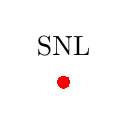
\begin{tikzpicture}

\begin{axis}[%
width=0.96731\figurewidth,
height=\figureheight,
at={(0\figurewidth,0\figureheight)},
scale only axis,
unbounded coords=jump,
every outer x axis line/.append style={black},
every x tick label/.append style={font=\color{black}},
xtick={0,0.1},
xmin=-0.00576036866359447,
xmax=0.102534562211982,
xlabel={freq},
every outer y axis line/.append style={black},
every y tick label/.append style={font=\color{black}},
ymin=-341.742848099994,
ymax=18.7034306519713,
ylabel={Amplitude},
title={SNL},
axis x line*=bottom,
axis y line*=left
]
\addplot [color=blue,only marks,mark=o,mark options={solid},forget plot]
  table[row sep=crcr]{%
0.000244140625	8.55350673954086\\
0.00048828125	8.55590581262265\\
0.000732421875	8.56397495782221\\
0.0009765625	8.56636903193436\\
0.001220703125	8.55225563128596\\
0.00146484375	8.56189590780002\\
0.001708984375	8.55379296549472\\
0.001953125	8.55120958421702\\
0.002197265625	8.56455148277672\\
0.00244140625	8.55931021686109\\
0.002685546875	8.55485500239587\\
0.0029296875	8.5604280071118\\
0.003173828125	8.54849415831177\\
0.00341796875	8.56339717713888\\
0.003662109375	8.56241192542848\\
0.00390625	8.55807509740657\\
0.004150390625	8.55720944514985\\
0.00439453125	8.55588796719661\\
0.004638671875	8.5646038987087\\
0.0048828125	8.56654164263676\\
0.005126953125	8.55105702891905\\
0.00537109375	8.55073693326733\\
0.005615234375	8.55950799849091\\
0.005859375	8.55975029145452\\
0.006103515625	8.56397635797498\\
0.00634765625	8.56073412985819\\
0.006591796875	8.55857627152284\\
0.0068359375	8.55464225471752\\
0.007080078125	8.55255738165187\\
0.00732421875	8.55954649259326\\
0.007568359375	8.55628452600342\\
0.0078125	8.55706685514207\\
0.008056640625	8.56142095557459\\
0.00830078125	8.55252209256406\\
0.008544921875	8.5502466415644\\
0.0087890625	8.55282902071326\\
0.009033203125	8.55437797072062\\
0.00927734375	8.56067050378067\\
0.009521484375	8.56029676269497\\
0.009765625	8.56849189118986\\
0.010009765625	8.55737624507816\\
0.01025390625	8.5665969029742\\
0.010498046875	8.56075305495699\\
0.0107421875	8.56163074961978\\
0.010986328125	8.56096172359332\\
0.01123046875	8.55497702388669\\
0.011474609375	8.55561679532605\\
0.01171875	8.56238315585193\\
0.011962890625	8.54905384787128\\
0.01220703125	8.55233340153046\\
0.012451171875	8.55774842522396\\
0.0126953125	8.55705257590961\\
0.012939453125	8.5545293027846\\
0.01318359375	8.55478151860007\\
0.013427734375	8.56131976515445\\
0.013671875	8.56518187191921\\
0.013916015625	8.56052439279443\\
0.01416015625	8.56330057791422\\
0.014404296875	8.56297272964957\\
0.0146484375	8.55221228993105\\
0.014892578125	8.55553382998113\\
0.01513671875	8.5550881442677\\
0.015380859375	8.56503732196256\\
0.015625	8.56256741581211\\
0.015869140625	8.55278916296726\\
0.01611328125	8.55566384659403\\
0.016357421875	8.55762263841655\\
0.0166015625	8.56318117882842\\
0.016845703125	8.55640062467546\\
0.01708984375	8.5544253076211\\
0.017333984375	8.55913796279862\\
0.017578125	8.56306978167004\\
0.017822265625	8.55798752255589\\
0.01806640625	8.56569345572058\\
0.018310546875	8.5457663480251\\
0.0185546875	8.5537986858954\\
0.018798828125	8.55861503985682\\
0.01904296875	8.56057918638953\\
0.019287109375	8.56083452273276\\
0.01953125	8.56054581584948\\
0.019775390625	8.56006425292429\\
0.02001953125	8.56309373667608\\
0.020263671875	8.56703195285968\\
0.0205078125	8.55429108198058\\
0.020751953125	8.55792472584079\\
0.02099609375	8.56439437997847\\
0.021240234375	8.56426573433316\\
0.021484375	8.55429863237089\\
0.021728515625	8.55346134233082\\
0.02197265625	8.56556163721547\\
0.022216796875	8.56394283499668\\
0.0224609375	8.55544477824645\\
0.022705078125	8.56099575968295\\
0.02294921875	8.56665275287457\\
0.023193359375	8.5655583271548\\
0.0234375	8.567152132096\\
0.023681640625	8.56174955260116\\
0.02392578125	8.5627452839795\\
0.024169921875	8.56114241468146\\
0.0244140625	8.56490250407217\\
0.024658203125	8.55166990438323\\
0.02490234375	8.55848361785735\\
0.025146484375	-308.226004638934\\
0.025390625	-319.791010966599\\
0.025634765625	-304.521000032424\\
0.02587890625	-306.612649060923\\
0.026123046875	-304.480069463168\\
0.0263671875	-307.8319312525\\
0.026611328125	-309.179120711577\\
0.02685546875	-304.092854040447\\
0.027099609375	-310.957131048929\\
0.02734375	-315.052422752546\\
0.027587890625	-313.190176923547\\
0.02783203125	-321.625587606638\\
0.028076171875	-307.825399879466\\
0.0283203125	-309.729463556496\\
0.028564453125	-316.362573414479\\
0.02880859375	-317.497285329506\\
0.029052734375	-311.264397643858\\
0.029296875	-322.766233391013\\
0.029541015625	-313.303595914686\\
0.02978515625	-307.245059067252\\
0.030029296875	-315.032004437237\\
0.0302734375	-312.920743887868\\
0.030517578125	-313.898038475724\\
0.03076171875	-320.948843592125\\
0.031005859375	-313.635313564157\\
0.03125	-324.506337705425\\
0.031494140625	-311.077101637184\\
0.03173828125	-317.147475198062\\
0.031982421875	-313.575348931025\\
0.0322265625	-329.082101868917\\
0.032470703125	-321.786322260458\\
0.03271484375	-318.766966168387\\
0.032958984375	-314.342571051545\\
0.033203125	-317.399338009446\\
0.033447265625	-309.799526781294\\
0.03369140625	-313.463452027975\\
0.033935546875	-316.9223827019\\
0.0341796875	-315.663816472031\\
0.034423828125	-309.218913386684\\
0.03466796875	-309.533865237357\\
0.034912109375	-309.953262560731\\
0.03515625	-314.866414247159\\
0.035400390625	-316.98069248758\\
0.03564453125	-311.608701300114\\
0.035888671875	-314.963708362321\\
0.0361328125	-314.835534005254\\
0.036376953125	-314.878717794919\\
0.03662109375	-316.508046952085\\
0.036865234375	-315.703496259141\\
0.037109375	-333.028120172213\\
0.037353515625	-311.669404943713\\
0.03759765625	-312.10209536046\\
0.037841796875	-325.1123953171\\
0.0380859375	-319.09179540382\\
0.038330078125	-307.050595577261\\
0.03857421875	-306.787306190037\\
0.038818359375	-304.581610882266\\
0.0390625	-312.807906103317\\
0.039306640625	-319.09179540382\\
0.03955078125	-307.952361880752\\
0.039794921875	-303.40977816315\\
0.0400390625	-310.060895533901\\
0.040283203125	-313.07119549054\\
0.04052734375	-307.050595577261\\
0.040771484375	-319.09179540382\\
nan	nan\\
0.041259765625	-321.960238249866\\
0.04150390625	-307.050595577261\\
0.041748046875	-305.1123953171\\
0.0419921875	-307.046356489741\\
0.042236328125	-309.51931520803\\
0.04248046875	-306.08149544718\\
0.042724609375	-312.807906103317\\
0.04296875	-319.09179540382\\
0.043212890625	-309.549370309427\\
0.04345703125	-313.07119549054\\
nan	nan\\
0.0439453125	-309.549370309427\\
0.044189453125	-313.07119549054\\
0.04443359375	-319.09179540382\\
0.044677734375	-310.332144379921\\
0.044921875	-319.09179540382\\
0.045166015625	-310.305141527215\\
0.04541015625	-331.132995230379\\
0.045654296875	-312.807906103317\\
0.0458984375	-313.07119549054\\
0.046142578125	-325.1123953171\\
0.04638671875	-308.461277946349\\
0.046630859375	-306.08149544718\\
0.046875	-317.092200819668\\
0.047119140625	-314.309096744798\\
0.04736328125	-321.356406930634\\
0.047607421875	-317.903818918079\\
0.0478515625	-313.667597737138\\
0.048095703125	-310.82262947639\\
0.04833984375	-316.491364206984\\
0.048583984375	-310.647942535076\\
0.048828125	-306.757082163626\\
0.049072265625	-312.709924768508\\
0.04931640625	-315.739932042868\\
0.049560546875	-310.356848202837\\
0.0498046875	-328.272067292964\\
0.050048828125	-308.115450303511\\
0.05029296875	-312.000752642666\\
0.050537109375	-312.98445977118\\
0.05078125	-309.215881428334\\
0.051025390625	-311.349946507933\\
0.05126953125	-318.601317929511\\
0.051513671875	-323.824538625492\\
0.0517578125	-318.536529472743\\
0.052001953125	-313.807776033038\\
0.05224609375	-311.061051581723\\
0.052490234375	-312.40511923358\\
0.052734375	-315.931240876393\\
0.052978515625	-309.663005373483\\
0.05322265625	-308.669976177031\\
0.053466796875	-316.707826333763\\
0.0537109375	-318.800437537408\\
0.053955078125	-307.69025491516\\
0.05419921875	-310.956796117199\\
0.054443359375	-306.740720378909\\
0.0546875	-316.451017693241\\
0.054931640625	-306.760647066199\\
0.05517578125	-311.135393463317\\
0.055419921875	-312.461141463871\\
0.0556640625	-322.172783334109\\
0.055908203125	-310.459926007421\\
0.05615234375	-315.452107961114\\
0.056396484375	-310.160511725858\\
0.056640625	-326.323909894344\\
0.056884765625	-320.304424062247\\
0.05712890625	-324.586922598025\\
0.057373046875	-309.540577707701\\
0.0576171875	-312.313938518167\\
0.057861328125	-312.840210561578\\
0.05810546875	-312.482913128453\\
0.058349609375	-315.215058842567\\
0.05859375	-336.988512817801\\
0.058837890625	-313.013174465972\\
0.05908203125	-315.323043020818\\
0.059326171875	-329.836252107513\\
0.0595703125	-312.843207448756\\
0.059814453125	-315.500599705993\\
0.06005859375	-315.319256400951\\
0.060302734375	-312.974847083585\\
0.060546875	-312.518467631408\\
0.060791015625	-318.795219272641\\
0.06103515625	-315.127273895056\\
0.061279296875	-319.773374288619\\
0.0615234375	-311.398958006308\\
0.061767578125	-318.961436851172\\
0.06201171875	-307.690723268649\\
0.062255859375	-324.895614369408\\
0.0625	-318.931792385811\\
0.062744140625	-313.791866877524\\
0.06298828125	-323.062745762084\\
0.063232421875	-317.81903887586\\
0.0634765625	-313.693678543766\\
0.063720703125	-316.363582784729\\
0.06396484375	-307.660423785521\\
0.064208984375	-320.448743977808\\
0.064453125	-307.775563311059\\
0.064697265625	-334.398498471074\\
0.06494140625	-307.136695260897\\
0.065185546875	-307.886206003379\\
0.0654296875	-320.379797054456\\
0.065673828125	-316.672755373253\\
0.06591796875	-316.707600294625\\
0.066162109375	-306.71095255035\\
0.06640625	-312.063969365983\\
0.066650390625	-313.673802716354\\
0.06689453125	-320.180429098946\\
0.067138671875	-318.350050033588\\
0.0673828125	-321.53331161883\\
0.067626953125	-322.8309563474\\
0.06787109375	-312.397778335051\\
0.068115234375	-323.071558841613\\
0.068359375	-313.895844989518\\
0.068603515625	-327.00752185462\\
0.06884765625	-325.002366995448\\
0.069091796875	-322.807379869818\\
0.0693359375	-319.814622780142\\
0.069580078125	-308.752440494678\\
0.06982421875	-309.743628160795\\
0.070068359375	-317.431829056473\\
0.0703125	-320.409539488055\\
0.070556640625	-316.534253529521\\
0.07080078125	-319.562225688775\\
0.071044921875	-315.993462978558\\
0.0712890625	-321.67915334561\\
0.071533203125	-311.530880633266\\
0.07177734375	-312.724790281843\\
0.072021484375	-317.255192003317\\
0.072265625	-321.179334115284\\
0.072509765625	-313.626035457864\\
0.07275390625	-308.138347532613\\
0.072998046875	-315.815782190709\\
0.0732421875	-304.88582477878\\
0.073486328125	-315.732176008029\\
0.07373046875	-309.138356601021\\
0.073974609375	-312.134487375884\\
0.07421875	-317.725606216476\\
0.074462890625	-321.180161075464\\
0.07470703125	-319.391285718548\\
0.074951171875	-319.416487184779\\
0.0751953125	-320.190695176988\\
0.075439453125	-309.073358383897\\
0.07568359375	-309.572655064409\\
0.075927734375	-305.160157421186\\
0.076171875	-310.319589742456\\
0.076416015625	-310.485335349771\\
0.07666015625	-312.732154611256\\
0.076904296875	-307.256018387709\\
0.0771484375	-306.54231483019\\
0.077392578125	-322.419528658008\\
0.07763671875	-303.675554269078\\
0.077880859375	-307.16094384377\\
0.078125	-315.766042605044\\
0.078369140625	-309.875615142341\\
0.07861328125	-313.825250288856\\
0.078857421875	-310.686589935568\\
0.0791015625	-308.799567944684\\
0.079345703125	-314.051752925036\\
0.07958984375	-312.967675460751\\
0.079833984375	-316.113741008221\\
0.080078125	-306.446558096223\\
0.080322265625	-317.680616339876\\
0.08056640625	-312.009270240773\\
0.080810546875	-332.138921569402\\
0.0810546875	-316.620258677461\\
0.081298828125	-312.210576892494\\
0.08154296875	-316.92643825769\\
0.081787109375	-312.999598968908\\
0.08203125	-318.034846617694\\
0.082275390625	-323.586438499606\\
0.08251953125	-314.711938314365\\
0.082763671875	-312.591697646458\\
0.0830078125	-308.39775430044\\
0.083251953125	-314.19491121222\\
0.08349609375	-316.578282611462\\
0.083740234375	-314.150099326794\\
0.083984375	-314.926129298843\\
0.084228515625	-320.486704689421\\
0.08447265625	-313.451481513589\\
0.084716796875	-335.17953782616\\
0.0849609375	-311.901448726575\\
0.085205078125	-315.057025593391\\
0.08544921875	-316.492716371414\\
0.085693359375	-315.942145984147\\
0.0859375	-311.859173724187\\
0.086181640625	-315.680841135169\\
0.08642578125	-315.420720302379\\
0.086669921875	-315.758862828999\\
0.0869140625	-313.475333691849\\
0.087158203125	-310.866189518187\\
0.08740234375	-309.825173670595\\
0.087646484375	-309.86463328752\\
0.087890625	-326.196320607452\\
0.088134765625	-317.886139054003\\
0.08837890625	-311.619469291405\\
0.088623046875	-315.992530134719\\
0.0888671875	-319.875286781456\\
0.089111328125	-314.735886304747\\
0.08935546875	-324.461014258747\\
0.089599609375	-310.505667324923\\
0.08984375	-309.053101887918\\
0.090087890625	-325.202227300099\\
0.09033203125	-310.257201565836\\
0.090576171875	-312.678656280782\\
0.0908203125	-316.068258327069\\
0.091064453125	-316.900569642096\\
0.09130859375	-312.462538250446\\
0.091552734375	-307.347501452076\\
0.091796875	-310.151639853829\\
0.092041015625	-315.211478050516\\
0.09228515625	-311.661551495165\\
0.092529296875	-307.072693014169\\
0.0927734375	-328.766624219249\\
0.093017578125	-310.283431177704\\
0.09326171875	-323.209500876295\\
0.093505859375	-321.892892522477\\
0.09375	-321.560561716326\\
0.093994140625	-310.762804527458\\
0.09423828125	-312.298728339527\\
0.094482421875	-324.290593161113\\
0.0947265625	-318.381109496037\\
0.094970703125	-314.594802414218\\
0.09521484375	-312.663287040882\\
0.095458984375	-315.652530826615\\
0.095703125	-318.844206065898\\
0.095947265625	-317.440145436689\\
0.09619140625	-312.836613778798\\
0.096435546875	-307.480913250724\\
0.0966796875	-305.157635604416\\
0.096923828125	-308.801095163579\\
0.09716796875	-308.347951657188\\
0.097412109375	-308.471912945222\\
0.09765625	-314.405967673374\\
0.097900390625	-323.971038518812\\
0.09814453125	-314.64787179143\\
0.098388671875	-314.811459444794\\
0.0986328125	-315.644926948598\\
0.098876953125	-317.762056316609\\
0.09912109375	-322.689988178272\\
0.099365234375	-315.23465576589\\
0.099609375	-321.019621219149\\
0.099853515625	-319.456522193474\\
0.10009765625	-310.642115249032\\
0.100341796875	-310.656527883585\\
0.1005859375	-311.888847698003\\
0.100830078125	-316.810485666217\\
0.10107421875	-315.496722769499\\
0.101318359375	-317.780116552719\\
0.1015625	-311.173010026333\\
0.101806640625	-310.606470771608\\
0.10205078125	-310.20666045155\\
0.102294921875	-313.66523356021\\
0.1025390625	-314.83801659319\\
};
\addplot [color=black!50!green,only marks,mark=*,mark options={solid},forget plot]
  table[row sep=crcr]{%
0.000244140625	8.55350673954086\\
0.00048828125	8.55590581262265\\
0.000732421875	8.56397495782221\\
0.0009765625	8.56636903193436\\
0.001220703125	8.55225563128596\\
0.00146484375	8.56189590780002\\
0.001708984375	8.55379296549472\\
0.001953125	8.55120958421702\\
0.002197265625	8.56455148277672\\
0.00244140625	8.55931021686109\\
0.002685546875	8.55485500239587\\
0.0029296875	8.5604280071118\\
0.003173828125	8.54849415831177\\
0.00341796875	8.56339717713888\\
0.003662109375	8.56241192542853\\
0.00390625	8.55807509740657\\
0.004150390625	8.55720944514985\\
0.00439453125	8.55588796719661\\
0.004638671875	8.5646038987087\\
0.0048828125	8.56654164263676\\
0.005126953125	8.55105702891905\\
0.00537109375	8.55073693326733\\
0.005615234375	8.55950799849091\\
0.005859375	8.55975029145452\\
0.006103515625	8.56397635797498\\
0.00634765625	8.56073412985819\\
0.006591796875	8.55857627152284\\
0.0068359375	8.55464225471752\\
0.007080078125	8.55255738165187\\
0.00732421875	8.55954649259326\\
0.007568359375	8.55628452600342\\
0.0078125	8.55706685514207\\
0.008056640625	8.56142095557459\\
0.00830078125	8.55252209256406\\
0.008544921875	8.5502466415644\\
0.0087890625	8.55282902071326\\
0.009033203125	8.55437797072062\\
0.00927734375	8.56067050378067\\
0.009521484375	8.56029676269497\\
0.009765625	8.56849189118986\\
0.010009765625	8.55737624507816\\
0.01025390625	8.5665969029742\\
0.010498046875	8.56075305495699\\
0.0107421875	8.56163074961978\\
0.010986328125	8.56096172359332\\
0.01123046875	8.55497702388669\\
0.011474609375	8.55561679532605\\
0.01171875	8.56238315585193\\
0.011962890625	8.54905384787128\\
0.01220703125	8.55233340153046\\
0.012451171875	8.55774842522396\\
0.0126953125	8.55705257590961\\
0.012939453125	8.55452930278466\\
0.01318359375	8.55478151860007\\
0.013427734375	8.56131976515445\\
0.013671875	8.56518187191921\\
0.013916015625	8.56052439279443\\
0.01416015625	8.56330057791422\\
0.014404296875	8.56297272964957\\
0.0146484375	8.55221228993105\\
0.014892578125	8.55553382998113\\
0.01513671875	8.5550881442677\\
0.015380859375	8.56503732196256\\
0.015625	8.56256741581211\\
0.015869140625	8.55278916296726\\
0.01611328125	8.55566384659403\\
0.016357421875	8.55762263841655\\
0.0166015625	8.56318117882842\\
0.016845703125	8.55640062467546\\
0.01708984375	8.5544253076211\\
0.017333984375	8.55913796279862\\
0.017578125	8.56306978167004\\
0.017822265625	8.55798752255589\\
0.01806640625	8.56569345572058\\
0.018310546875	8.5457663480251\\
0.0185546875	8.5537986858954\\
0.018798828125	8.55861503985682\\
0.01904296875	8.56057918638953\\
0.019287109375	8.56083452273276\\
0.01953125	8.56054581584948\\
0.019775390625	8.56006425292429\\
0.02001953125	8.56309373667608\\
0.020263671875	8.56703195285968\\
0.0205078125	8.55429108198058\\
0.020751953125	8.55792472584079\\
0.02099609375	8.56439437997847\\
0.021240234375	8.56426573433316\\
0.021484375	8.55429863237089\\
0.021728515625	8.55346134233082\\
0.02197265625	8.56556163721547\\
0.022216796875	8.56394283499668\\
0.0224609375	8.55544477824645\\
0.022705078125	8.56099575968295\\
0.02294921875	8.56665275287457\\
0.023193359375	8.5655583271548\\
0.0234375	8.567152132096\\
0.023681640625	8.56174955260116\\
0.02392578125	8.5627452839795\\
0.024169921875	8.56114241468146\\
0.0244140625	8.56490250407217\\
0.024658203125	8.55166990438323\\
0.02490234375	8.55848361785735\\
0.025146484375	-311.434042098426\\
0.025390625	-314.490094583876\\
0.025634765625	-307.914677175221\\
0.02587890625	-310.402585291898\\
0.026123046875	-305.820917606603\\
0.0263671875	-310.776027472262\\
0.026611328125	-310.295025328976\\
0.02685546875	-303.124578000092\\
0.027099609375	-331.370261575289\\
0.02734375	-319.374831017504\\
0.027587890625	-311.883797126073\\
0.02783203125	-312.807831151416\\
0.028076171875	-306.926985447065\\
0.0283203125	-311.069985741456\\
0.028564453125	-324.721896131877\\
0.02880859375	-317.593504056448\\
0.029052734375	-312.504426505466\\
0.029296875	-323.515478736182\\
0.029541015625	-313.241094758796\\
0.02978515625	-304.740784771739\\
0.030029296875	-314.887190355334\\
0.0302734375	-313.928837858823\\
0.030517578125	-309.291922301106\\
0.03076171875	-314.775365663777\\
0.031005859375	-314.547659394721\\
0.03125	-313.384379963109\\
0.031494140625	-310.979749966906\\
0.03173828125	-314.704012924397\\
0.031982421875	-312.185980407525\\
0.0322265625	-327.913843779055\\
0.032470703125	-319.245826337884\\
0.03271484375	-314.063055566547\\
0.032958984375	-317.007456278745\\
0.033203125	-318.055368240584\\
0.033447265625	-310.510242884779\\
0.03369140625	-315.76208485266\\
0.033935546875	-314.180794347219\\
0.0341796875	-315.702569656517\\
0.034423828125	-316.068584853556\\
0.03466796875	-309.734440502876\\
0.034912109375	-311.428993182671\\
0.03515625	-317.950814791699\\
0.035400390625	-321.144430481685\\
0.03564453125	-316.051915090527\\
0.035888671875	-318.057751791464\\
0.0361328125	-314.159646988173\\
0.036376953125	-309.885603354816\\
0.03662109375	-317.770482765553\\
0.036865234375	-312.51772762208\\
0.037109375	-338.814797407462\\
0.037353515625	-311.343477804895\\
0.03759765625	-312.10209536046\\
0.037841796875	-303.40977816315\\
nan	nan\\
0.038330078125	-313.07119549054\\
0.03857421875	-313.07119549054\\
0.038818359375	-302.963956836623\\
0.0390625	-319.09179540382\\
0.039306640625	-311.132995230379\\
0.03955078125	-307.952361880752\\
0.039794921875	-303.40977816315\\
0.0400390625	-313.07119549054\\
0.040283203125	-306.08149544718\\
0.04052734375	-313.07119549054\\
0.040771484375	-306.983261750671\\
0.041015625	-313.07119549054\\
0.041259765625	-306.960809133134\\
0.04150390625	-312.10209536046\\
0.041748046875	-314.231034430094\\
0.0419921875	-320.251634343374\\
0.042236328125	-313.631769962545\\
0.04248046875	-312.666531944608\\
0.042724609375	-321.590570135986\\
0.04296875	-312.10209536046\\
0.043212890625	-307.050595577261\\
0.04345703125	-319.09179540382\\
0.043701171875	-307.050595577261\\
0.0439453125	-312.10209536046\\
0.044189453125	-319.09179540382\\
0.04443359375	-307.050595577261\\
0.044677734375	-309.250743503326\\
0.044921875	-313.07119549054\\
0.045166015625	-313.07119549054\\
0.04541015625	-307.050595577261\\
0.045654296875	-312.10209536046\\
0.0458984375	-316.08149544718\\
0.046142578125	-319.09179540382\\
0.04638671875	-312.048145041593\\
0.046630859375	-305.1123953171\\
0.046875	-315.366469559518\\
0.047119140625	-312.793912036776\\
0.04736328125	-313.288740124089\\
0.047607421875	-310.149488868823\\
0.0478515625	-312.595135042771\\
0.048095703125	-320.389186275481\\
0.04833984375	-313.707974811996\\
0.048583984375	-313.067282028164\\
0.048828125	-316.1594029674\\
0.049072265625	-314.472888470115\\
0.04931640625	-326.274841064839\\
0.049560546875	-309.083352692195\\
0.0498046875	-316.806989671526\\
0.050048828125	-310.08635710952\\
0.05029296875	-325.662292165697\\
0.050537109375	-310.971035034401\\
0.05078125	-311.115774424603\\
0.051025390625	-305.600587508883\\
0.05126953125	-312.033825075313\\
0.051513671875	-311.249338161196\\
0.0517578125	-312.664396633593\\
0.052001953125	-317.244886282587\\
0.05224609375	-314.505901797571\\
0.052490234375	-314.50080595656\\
0.052734375	-310.715995429571\\
0.052978515625	-308.002955977851\\
0.05322265625	-309.107950947251\\
0.053466796875	-310.91569968443\\
0.0537109375	-316.352667574072\\
0.053955078125	-309.454018349658\\
0.05419921875	-309.650861310353\\
0.054443359375	-306.834237296985\\
0.0546875	-312.595903655027\\
0.054931640625	-306.410043433748\\
0.05517578125	-322.266986845565\\
0.055419921875	-308.843764938902\\
0.0556640625	-313.072539644043\\
0.055908203125	-313.258658706593\\
0.05615234375	-315.740793512492\\
0.056396484375	-315.030040593643\\
0.056640625	-319.813410710305\\
0.056884765625	-326.604944704811\\
0.05712890625	-311.255697191232\\
0.057373046875	-308.72557183156\\
0.0576171875	-309.609413829263\\
0.057861328125	-312.845126087464\\
0.05810546875	-310.883087887949\\
0.058349609375	-313.885729915342\\
0.05859375	-318.345382901231\\
0.058837890625	-316.922872398027\\
0.05908203125	-311.79585616319\\
0.059326171875	-318.85566895259\\
0.0595703125	-308.842652006088\\
0.059814453125	-316.487237628011\\
0.06005859375	-311.134802118575\\
0.060302734375	-311.787562483555\\
0.060546875	-314.024395553648\\
0.060791015625	-314.640190205907\\
0.06103515625	-321.610091397782\\
0.061279296875	-323.315789900086\\
0.0615234375	-307.743569889479\\
0.061767578125	-317.89386780728\\
0.06201171875	-307.988136426891\\
0.062255859375	-318.692739414247\\
0.0625	-315.930750238395\\
0.062744140625	-313.154312407504\\
0.06298828125	-321.80365117871\\
0.063232421875	-313.913176472859\\
0.0634765625	-324.63467229635\\
0.063720703125	-312.192376100965\\
0.06396484375	-308.568649259054\\
0.064208984375	-312.875152480487\\
0.064453125	-316.016527285703\\
0.064697265625	-329.875321628739\\
0.06494140625	-306.302754184229\\
0.065185546875	-313.395388099714\\
0.0654296875	-325.657272980574\\
0.065673828125	-313.161682921412\\
0.06591796875	-315.992798413913\\
0.066162109375	-311.844672835937\\
0.06640625	-310.552064414699\\
0.066650390625	-311.59376167361\\
0.06689453125	-328.881931898862\\
0.067138671875	-311.783335917736\\
0.0673828125	-317.069199568617\\
0.067626953125	-310.640527598589\\
0.06787109375	-317.39888226431\\
0.068115234375	-323.022401217161\\
0.068359375	-315.631737447864\\
0.068603515625	-315.462108391055\\
0.06884765625	-312.235936619237\\
0.069091796875	-313.567515965765\\
0.0693359375	-311.313058655379\\
0.069580078125	-315.774838053075\\
0.06982421875	-314.359889224812\\
0.070068359375	-315.185888863108\\
0.0703125	-318.490355036383\\
0.070556640625	-320.682449765102\\
0.07080078125	-313.962018493226\\
0.071044921875	-322.979328747262\\
0.0712890625	-324.46515937538\\
0.071533203125	-317.615462471003\\
0.07177734375	-315.041771391868\\
0.072021484375	-313.953112631592\\
0.072265625	-313.443070265363\\
0.072509765625	-321.776035685164\\
0.07275390625	-307.993211235656\\
0.072998046875	-307.464259969975\\
0.0732421875	-304.757502780489\\
0.073486328125	-319.359315206172\\
0.07373046875	-307.580494662296\\
0.073974609375	-315.656797056505\\
0.07421875	-315.100719924605\\
0.074462890625	-321.46743763639\\
0.07470703125	-318.585089186169\\
0.074951171875	-311.496914157447\\
0.0751953125	-311.568659514091\\
0.075439453125	-310.595373472295\\
0.07568359375	-307.818036887975\\
0.075927734375	-305.445562699589\\
0.076171875	-308.160544881159\\
0.076416015625	-306.969262069444\\
0.07666015625	-311.752702219559\\
0.076904296875	-308.956834494186\\
0.0771484375	-306.615978067439\\
0.077392578125	-324.424919635037\\
0.07763671875	-303.480295123795\\
0.077880859375	-309.054197897663\\
0.078125	-312.445652839854\\
0.078369140625	-305.875456088654\\
0.07861328125	-314.873718611816\\
0.078857421875	-326.004864547673\\
0.0791015625	-314.599098426629\\
0.079345703125	-322.185551801421\\
0.07958984375	-310.326286738974\\
0.079833984375	-313.987312657791\\
0.080078125	-310.852651509642\\
0.080322265625	-318.906913790397\\
0.08056640625	-311.24026107243\\
0.080810546875	-323.34977917779\\
0.0810546875	-312.992556765616\\
0.081298828125	-311.902418039449\\
0.08154296875	-316.21089846869\\
0.081787109375	-322.224978512637\\
0.08203125	-315.141720176462\\
0.082275390625	-311.435860967037\\
0.08251953125	-315.59940082997\\
0.082763671875	-329.529847181985\\
0.0830078125	-310.553977919194\\
0.083251953125	-328.242482355774\\
0.08349609375	-311.275297840138\\
0.083740234375	-312.454955559295\\
0.083984375	-314.370496545016\\
0.084228515625	-310.03115963276\\
0.08447265625	-320.979089634108\\
0.084716796875	-313.838607403199\\
0.0849609375	-312.727971966443\\
0.085205078125	-313.325467585706\\
0.08544921875	-312.952058588525\\
0.085693359375	-311.844842607609\\
0.0859375	-312.796189677957\\
0.086181640625	-311.277927127949\\
0.08642578125	-317.308937858612\\
0.086669921875	-314.079291874863\\
0.0869140625	-312.668988950907\\
0.087158203125	-310.04623802175\\
0.08740234375	-312.606603706738\\
0.087646484375	-309.783637697212\\
0.087890625	-312.947166337383\\
0.088134765625	-312.601668655559\\
0.08837890625	-316.87859664067\\
0.088623046875	-314.598293165497\\
0.0888671875	-320.209436599307\\
0.089111328125	-309.579789646003\\
0.08935546875	-325.238484548565\\
0.089599609375	-313.811705438549\\
0.08984375	-308.125812552027\\
0.090087890625	-313.12384861152\\
0.09033203125	-319.978367829896\\
0.090576171875	-306.574500925363\\
0.0908203125	-313.880037383452\\
0.091064453125	-313.226671520762\\
0.09130859375	-310.797982205575\\
0.091552734375	-312.307457640728\\
0.091796875	-310.603068168081\\
0.092041015625	-309.439920603244\\
0.09228515625	-309.199116430382\\
0.092529296875	-307.843907279366\\
0.0927734375	-318.467091077015\\
0.093017578125	-314.721270510218\\
0.09326171875	-322.633693723727\\
0.093505859375	-315.308324748557\\
0.09375	-327.206543956555\\
0.093994140625	-313.015939428964\\
0.09423828125	-313.925150984725\\
0.094482421875	-314.298752421966\\
0.0947265625	-315.08458234981\\
0.094970703125	-314.389696853644\\
0.09521484375	-309.892457547149\\
0.095458984375	-311.864656535231\\
0.095703125	-319.316289680754\\
0.095947265625	-335.785067216553\\
0.09619140625	-314.466963588431\\
0.096435546875	-307.315979381025\\
0.0966796875	-306.96439185573\\
0.096923828125	-309.512461685551\\
0.09716796875	-306.978103385801\\
0.097412109375	-306.509106120431\\
0.09765625	-311.072011474133\\
0.097900390625	-320.206131650253\\
0.09814453125	-316.043434461472\\
0.098388671875	-311.653965320777\\
0.0986328125	-315.18272799906\\
0.098876953125	-312.264914527244\\
0.09912109375	-314.089117630782\\
0.099365234375	-316.845088418086\\
0.099609375	-319.009920223629\\
0.099853515625	-311.511982926293\\
0.10009765625	-114.455922235248\\
0.100341796875	-116.269138084271\\
0.1005859375	-118.271618333062\\
0.100830078125	-112.04572736784\\
0.10107421875	-110.846359228952\\
0.101318359375	-113.049550065086\\
0.1015625	-125.93561598655\\
0.101806640625	-120.611669176763\\
0.10205078125	-117.279319025283\\
0.102294921875	-119.054236445743\\
0.1025390625	-125.57979828686\\
};
\addplot [color=red,only marks,mark=*,mark options={solid},forget plot]
  table[row sep=crcr]{%
0.000244140625	8.56068421913295\\
0.00048828125	8.55989436404724\\
0.000732421875	8.5610168209916\\
0.0009765625	8.58343323829604\\
0.001220703125	8.57567604133959\\
0.00146484375	8.55860783133312\\
0.001708984375	8.57963205139197\\
0.001953125	8.56719843392887\\
0.002197265625	8.55708425649038\\
0.00244140625	8.5541522800587\\
0.002685546875	8.5564824150224\\
0.0029296875	8.54377733065292\\
0.003173828125	8.54721210675177\\
0.00341796875	8.54863324407188\\
0.003662109375	8.57287974902425\\
0.00390625	8.55847170288769\\
0.004150390625	8.57169157216799\\
0.00439453125	8.56800921052002\\
0.004638671875	8.5496510302122\\
0.0048828125	8.55836129510737\\
0.005126953125	8.55119191146099\\
0.00537109375	8.55273173614398\\
0.005615234375	8.5690984997712\\
0.005859375	8.57696160544907\\
0.006103515625	8.5925530069693\\
0.00634765625	8.55891033649795\\
0.006591796875	8.5544887072939\\
0.0068359375	8.57854436555454\\
0.007080078125	8.56846077544321\\
0.00732421875	8.55760176674966\\
0.007568359375	8.56497471314322\\
0.0078125	8.57120185795685\\
0.008056640625	8.57744319126618\\
0.00830078125	8.55263500065536\\
0.008544921875	8.54903405471765\\
0.0087890625	8.56339400254473\\
0.009033203125	8.5597628365058\\
0.00927734375	8.54859992427276\\
0.009521484375	8.56631850949179\\
0.009765625	8.57525464913709\\
0.010009765625	8.58436122826834\\
0.01025390625	8.56640483486916\\
0.010498046875	8.57235844647278\\
0.0107421875	8.56560698321067\\
0.010986328125	8.55201640136215\\
0.01123046875	8.56189308761185\\
0.011474609375	8.56482219905655\\
0.01171875	8.56661152753446\\
0.011962890625	8.55555243107329\\
0.01220703125	8.55398091512694\\
0.012451171875	8.57578355698155\\
0.0126953125	8.55183694843817\\
0.012939453125	8.5863892602743\\
0.01318359375	8.56038357911569\\
0.013427734375	8.55051656399087\\
0.013671875	8.5683718812885\\
0.013916015625	8.56674256485388\\
0.01416015625	8.56518723200043\\
0.014404296875	8.55056361518263\\
0.0146484375	8.54646349317977\\
0.014892578125	8.53738947895999\\
0.01513671875	8.57025614543943\\
0.015380859375	8.55585872598471\\
0.015625	8.58010163674169\\
0.015869140625	8.56298894396559\\
0.01611328125	8.5718311810877\\
0.016357421875	8.55206745467638\\
0.0166015625	8.55247527940088\\
0.016845703125	8.57292307673532\\
0.01708984375	8.5450288481984\\
0.017333984375	8.5530686437657\\
0.017578125	8.57804722260119\\
0.017822265625	8.56822274949161\\
0.01806640625	8.55584060777051\\
0.018310546875	8.54488942190795\\
0.0185546875	8.54650667736809\\
0.018798828125	8.55812182486653\\
0.01904296875	8.56926269524621\\
0.019287109375	8.55804113211667\\
0.01953125	8.5681120940402\\
0.019775390625	8.5681484840531\\
0.02001953125	8.57742623008932\\
0.020263671875	8.59692815038045\\
0.0205078125	8.59128051906623\\
0.020751953125	8.55940477791711\\
0.02099609375	8.55196634372851\\
0.021240234375	8.56098933636531\\
0.021484375	8.57273202164657\\
0.021728515625	8.54916134005396\\
0.02197265625	8.57331799597762\\
0.022216796875	8.5435596600712\\
0.0224609375	8.55433150511357\\
0.022705078125	8.56104034295299\\
0.02294921875	8.55472841035845\\
0.023193359375	8.56582609376892\\
0.0234375	8.55668851261186\\
0.023681640625	8.56106355042567\\
0.02392578125	8.58783036903822\\
0.024169921875	8.57100590864377\\
0.0244140625	8.55071615016385\\
0.024658203125	8.56650580296241\\
0.02490234375	8.57097995403296\\
0.025146484375	-50.526364315644\\
0.025390625	-53.5852070491386\\
0.025634765625	-61.0502888078273\\
0.02587890625	-50.4811533966098\\
0.026123046875	-48.6916579447315\\
0.0263671875	-47.138495698973\\
0.026611328125	-47.6512087630425\\
0.02685546875	-51.30563719202\\
0.027099609375	-47.1539834049827\\
0.02734375	-48.0404041921871\\
0.027587890625	-60.2270657560048\\
0.02783203125	-44.6207636420738\\
0.028076171875	-60.2243855642417\\
0.0283203125	-45.0886932018596\\
0.028564453125	-47.8980946041339\\
0.02880859375	-54.875725122792\\
0.029052734375	-47.0835243131718\\
0.029296875	-49.7027970361223\\
0.029541015625	-49.3343478372664\\
0.02978515625	-46.4845290281141\\
0.030029296875	-45.9057948860622\\
0.0302734375	-50.1561765487371\\
0.030517578125	-50.3133203703524\\
0.03076171875	-53.8066810499145\\
0.031005859375	-55.3409529317042\\
0.03125	-63.671502044984\\
0.031494140625	-60.2485681264712\\
0.03173828125	-52.9135565294425\\
0.031982421875	-56.8716630353203\\
0.0322265625	-49.5185028567475\\
0.032470703125	-46.79710908956\\
0.03271484375	-47.4135476976145\\
0.032958984375	-57.1421510191409\\
0.033203125	-51.6882094057079\\
0.033447265625	-51.9629796652549\\
0.03369140625	-53.6697980243918\\
0.033935546875	-59.5059891140872\\
0.0341796875	-47.090021182266\\
0.034423828125	-56.201549612744\\
0.03466796875	-46.3208278431569\\
0.034912109375	-47.290735339629\\
0.03515625	-49.8243295393027\\
0.035400390625	-67.4780594821235\\
0.03564453125	-62.8291963714363\\
0.035888671875	-47.2757157311557\\
0.0361328125	-44.1077042735492\\
0.036376953125	-51.9735832038189\\
0.03662109375	-52.1913263255323\\
0.036865234375	-47.6460265341312\\
0.037109375	-54.2313582059771\\
0.037353515625	-49.6546251858625\\
0.03759765625	-60.2561677846587\\
0.037841796875	-51.6539151500928\\
0.0380859375	-52.2615830855407\\
0.038330078125	-50.1157505129399\\
0.03857421875	-46.5292152884461\\
0.038818359375	-50.2014864145052\\
0.0390625	-48.375895818244\\
0.039306640625	-55.0540407005511\\
0.03955078125	-51.5897670358306\\
0.039794921875	-55.8574637782111\\
0.0400390625	-47.8006517052205\\
0.040283203125	-46.979355713923\\
0.04052734375	-56.3886999498225\\
0.040771484375	-46.0717036816577\\
0.041015625	-71.6479397842029\\
0.041259765625	-61.9165630374434\\
0.04150390625	-47.1741660583106\\
0.041748046875	-46.394887209446\\
0.0419921875	-51.6222036256119\\
0.042236328125	-54.0571528179449\\
0.04248046875	-62.6693729618261\\
0.042724609375	-62.5412976722396\\
0.04296875	-53.4716956152801\\
0.043212890625	-51.0492032965981\\
0.04345703125	-49.3858099623572\\
0.043701171875	-50.7496895672438\\
0.0439453125	-46.8204011674362\\
0.044189453125	-49.3899393378599\\
0.04443359375	-59.7100823615182\\
0.044677734375	-57.7687939023943\\
0.044921875	-51.831412509948\\
0.045166015625	-54.9821841480128\\
0.04541015625	-48.6175300739258\\
0.045654296875	-54.8196638136149\\
0.0458984375	-52.0265459300872\\
0.046142578125	-49.9088399878011\\
0.04638671875	-48.3002092506644\\
0.046630859375	-50.4937019640886\\
0.046875	-59.6875729469984\\
0.047119140625	-54.4151951214414\\
0.04736328125	-70.9037560175209\\
0.047607421875	-49.6480088202566\\
0.0478515625	-45.4408960827745\\
0.048095703125	-67.5223007879412\\
0.04833984375	-53.9484401910967\\
0.048583984375	-51.3243102901018\\
0.048828125	-52.266814200481\\
0.049072265625	-50.864304185448\\
0.04931640625	-50.1735652904945\\
0.049560546875	-51.6144472174132\\
0.0498046875	-57.7976620657093\\
0.050048828125	-59.7183336449274\\
0.05029296875	-51.7005563504904\\
0.050537109375	-57.4398598771833\\
0.05078125	-57.6340540414802\\
0.051025390625	-54.648238782758\\
0.05126953125	-48.0927060933458\\
0.051513671875	-55.8105618517912\\
0.0517578125	-49.3225756621843\\
0.052001953125	-49.0770050074775\\
0.05224609375	-63.20736419152\\
0.052490234375	-52.0387632588042\\
0.052734375	-55.2118044886028\\
0.052978515625	-59.9755282580755\\
0.05322265625	-54.7413628763631\\
0.053466796875	-54.9959976702442\\
0.0537109375	-55.1072100245735\\
0.053955078125	-50.8515530108169\\
0.05419921875	-57.2062021533291\\
0.054443359375	-76.3002928191098\\
0.0546875	-54.1396158250981\\
0.054931640625	-54.7439705479071\\
0.05517578125	-50.6225450324471\\
0.055419921875	-56.8858781181184\\
0.0556640625	-63.9056330359404\\
0.055908203125	-61.422852288125\\
0.05615234375	-53.9201291825981\\
0.056396484375	-53.4201738176299\\
0.056640625	-60.6999765747273\\
0.056884765625	-59.5886799407816\\
0.05712890625	-53.4826354949033\\
0.057373046875	-59.4941099631968\\
0.0576171875	-60.0298266715381\\
0.057861328125	-52.8763018704051\\
0.05810546875	-53.3561721428506\\
0.058349609375	-56.5257284990691\\
0.05859375	-59.3526307367107\\
0.058837890625	-52.2418754058852\\
0.05908203125	-60.8116053477392\\
0.059326171875	-55.0605376304482\\
0.0595703125	-56.507101428952\\
0.059814453125	-57.0023321196496\\
0.06005859375	-56.7323973356721\\
0.060302734375	-54.4074656234837\\
0.060546875	-56.0094280526854\\
0.060791015625	-96.9297004591879\\
0.06103515625	-66.4114917781475\\
0.061279296875	-61.0731994662543\\
0.0615234375	-64.3043329285065\\
0.061767578125	-56.4931554048747\\
0.06201171875	-60.1986638862368\\
0.062255859375	-63.3481447342438\\
0.0625	-56.8965837980316\\
0.062744140625	-56.841831685529\\
0.06298828125	-68.6127855491658\\
0.063232421875	-59.7941791577663\\
0.0634765625	-67.678053676626\\
0.063720703125	-54.2776375953032\\
0.06396484375	-57.8440374681749\\
0.064208984375	-75.1026979724598\\
0.064453125	-61.5462199709253\\
0.064697265625	-60.6477305950868\\
0.06494140625	-62.4999924242486\\
0.065185546875	-61.5359695888924\\
0.0654296875	-58.8762016217273\\
0.065673828125	-62.5142585324746\\
0.06591796875	-67.6863154308723\\
0.066162109375	-62.5669494761555\\
0.06640625	-67.726200932207\\
0.066650390625	-69.6194846924168\\
0.06689453125	-68.1457269298535\\
0.067138671875	-56.2944968682881\\
0.0673828125	-58.6689988995386\\
0.067626953125	-68.4926425061476\\
0.06787109375	-56.5777099667237\\
0.068115234375	-58.0927440085499\\
0.068359375	-63.9105000549961\\
0.068603515625	-75.311226487123\\
0.06884765625	-65.1074895051394\\
0.069091796875	-67.5644849696894\\
0.0693359375	-71.8006987838883\\
0.069580078125	-64.3592277694818\\
0.06982421875	-66.6134355129895\\
0.070068359375	-66.5810444851767\\
0.0703125	-64.8084953346983\\
0.070556640625	-75.9641835300205\\
0.07080078125	-67.8085902953545\\
0.071044921875	-68.3159869217928\\
0.0712890625	-83.5740703785177\\
0.071533203125	-70.8685624530735\\
0.07177734375	-76.1330869464845\\
0.072021484375	-73.4751534576915\\
0.072265625	-69.7922941163711\\
0.072509765625	-71.2318121398146\\
0.07275390625	-72.6789624859324\\
0.072998046875	-73.0807995368866\\
0.0732421875	-70.3694149462419\\
0.073486328125	-73.2951348641648\\
0.07373046875	-76.4361732457815\\
0.073974609375	-77.7858754825421\\
0.07421875	-89.7708351538068\\
0.074462890625	-86.0362882178648\\
0.07470703125	-92.7514228879483\\
0.074951171875	-105.613886982688\\
0.0751953125	-103.555960082244\\
0.075439453125	-103.883726498963\\
0.07568359375	-107.864959373919\\
0.075927734375	-108.424232898317\\
0.076171875	-109.141147270838\\
0.076416015625	-127.047781512974\\
0.07666015625	-105.048730035649\\
0.076904296875	-103.035282662504\\
0.0771484375	-104.298045985055\\
0.077392578125	-103.926300849611\\
0.07763671875	-111.297886122932\\
0.077880859375	-108.275187502389\\
0.078125	-104.971067042275\\
0.078369140625	-102.734783352135\\
0.07861328125	-103.295940248597\\
0.078857421875	-101.33404965514\\
0.0791015625	-108.167970213839\\
0.079345703125	-102.03198664573\\
0.07958984375	-114.430552489753\\
0.079833984375	-108.121475964253\\
0.080078125	-117.866631476073\\
0.080322265625	-106.15030136725\\
0.08056640625	-105.315176518521\\
0.080810546875	-106.057627797051\\
0.0810546875	-140.289808845533\\
0.081298828125	-106.39185500335\\
0.08154296875	-110.168090545939\\
0.081787109375	-104.753429022148\\
0.08203125	-103.593156792999\\
0.082275390625	-107.590951971961\\
0.08251953125	-109.107834752624\\
0.082763671875	-118.709949949006\\
0.0830078125	-110.782347350882\\
0.083251953125	-108.207418773014\\
0.08349609375	-112.022755477553\\
0.083740234375	-110.65963977873\\
0.083984375	-106.770056376322\\
0.084228515625	-111.525396268426\\
0.08447265625	-106.885613435597\\
0.084716796875	-105.637057779463\\
0.0849609375	-114.79882330852\\
0.085205078125	-111.781044910144\\
0.08544921875	-110.511539722552\\
0.085693359375	-116.387963446881\\
0.0859375	-106.184725660629\\
0.086181640625	-112.549234303218\\
0.08642578125	-111.347146165223\\
0.086669921875	-109.095776852118\\
0.0869140625	-105.978866364876\\
0.087158203125	-116.727515840121\\
0.08740234375	-108.298177639934\\
0.087646484375	-113.856583467018\\
0.087890625	-114.962607578464\\
0.088134765625	-126.355356291148\\
0.08837890625	-112.376626418647\\
0.088623046875	-111.220415715523\\
0.0888671875	-108.406131135425\\
0.089111328125	-113.494810590982\\
0.08935546875	-108.02490855264\\
0.089599609375	-108.780587152044\\
0.08984375	-116.257160818411\\
0.090087890625	-113.942797942081\\
0.09033203125	-115.965367300753\\
0.090576171875	-115.169966921864\\
0.0908203125	-114.00312151569\\
0.091064453125	-113.278893539474\\
0.09130859375	-108.510063867913\\
0.091552734375	-107.308497876858\\
0.091796875	-113.329840298306\\
0.092041015625	-107.405887488317\\
0.09228515625	-107.656502452815\\
0.092529296875	-111.401758458743\\
0.0927734375	-119.907336243964\\
0.093017578125	-118.717605986437\\
0.09326171875	-114.037385094543\\
0.093505859375	-123.202139296521\\
0.09375	-115.420245828009\\
0.093994140625	-111.135860351579\\
0.09423828125	-110.824231396091\\
0.094482421875	-113.352585144165\\
0.0947265625	-112.009025966727\\
0.094970703125	-112.039438030648\\
0.09521484375	-119.641016342393\\
0.095458984375	-113.312589772041\\
0.095703125	-119.369921628526\\
0.095947265625	-122.121807431403\\
0.09619140625	-123.432220121643\\
0.096435546875	-117.517765404505\\
0.0966796875	-110.258032850823\\
0.096923828125	-109.372790253905\\
0.09716796875	-121.67297780285\\
0.097412109375	-109.51602611074\\
0.09765625	-111.929854426099\\
0.097900390625	-115.295221608865\\
0.09814453125	-116.093550506467\\
0.098388671875	-123.412352684054\\
0.0986328125	-113.526710990436\\
0.098876953125	-115.692384508063\\
0.09912109375	-129.076857980848\\
0.099365234375	-117.168468179306\\
0.099609375	-117.489115356756\\
0.099853515625	-117.613214669803\\
0.10009765625	-117.832183681075\\
0.100341796875	-119.515587871248\\
0.1005859375	-121.557348865947\\
0.100830078125	-115.505897528712\\
0.10107421875	-114.501340677024\\
0.101318359375	-116.896950059919\\
0.1015625	-129.363615228374\\
0.101806640625	-124.388546503922\\
0.10205078125	-120.784539301376\\
0.102294921875	-122.319636014696\\
0.1025390625	-128.400209590075\\
};
\end{axis}
\end{tikzpicture}%

		        \end{subfigure}%
		        ~ 
		        \begin{subfigure}[b]{0.3\textwidth}
		        	\centering
		            \setlength\figureheight{3cm} 
					\setlength\figurewidth{0.5\linewidth}
					% This file was created by matlab2tikz.
% Minimal pgfplots version: 1.3
%
%The latest updates can be retrieved from
%  http://www.mathworks.com/matlabcentral/fileexchange/22022-matlab2tikz
%where you can also make suggestions and rate matlab2tikz.
%
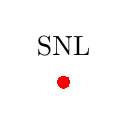
\begin{tikzpicture}

\begin{axis}[%
width=0.96731\figurewidth,
height=\figureheight,
at={(0\figurewidth,0\figureheight)},
scale only axis,
unbounded coords=jump,
every outer x axis line/.append style={black},
every x tick label/.append style={font=\color{black}},
xtick={0,0.1},
xmin=-0.00576036866359447,
xmax=0.102534562211982,
xlabel={freq},
every outer y axis line/.append style={black},
every y tick label/.append style={font=\color{black}},
ymin=-341.742848099994,
ymax=18.7034306519713,
ylabel={Amplitude},
title={SNL},
axis x line*=bottom,
axis y line*=left
]
\addplot [color=blue,only marks,mark=o,mark options={solid},forget plot]
  table[row sep=crcr]{%
0.000244140625	8.55350673954086\\
0.00048828125	8.55590581262265\\
0.000732421875	8.56397495782221\\
0.0009765625	8.56636903193436\\
0.001220703125	8.55225563128596\\
0.00146484375	8.56189590780002\\
0.001708984375	8.55379296549472\\
0.001953125	8.55120958421702\\
0.002197265625	8.56455148277672\\
0.00244140625	8.55931021686109\\
0.002685546875	8.55485500239587\\
0.0029296875	8.5604280071118\\
0.003173828125	8.54849415831177\\
0.00341796875	8.56339717713888\\
0.003662109375	8.56241192542848\\
0.00390625	8.55807509740657\\
0.004150390625	8.55720944514985\\
0.00439453125	8.55588796719661\\
0.004638671875	8.5646038987087\\
0.0048828125	8.56654164263676\\
0.005126953125	8.55105702891905\\
0.00537109375	8.55073693326733\\
0.005615234375	8.55950799849091\\
0.005859375	8.55975029145452\\
0.006103515625	8.56397635797498\\
0.00634765625	8.56073412985819\\
0.006591796875	8.55857627152284\\
0.0068359375	8.55464225471752\\
0.007080078125	8.55255738165187\\
0.00732421875	8.55954649259326\\
0.007568359375	8.55628452600342\\
0.0078125	8.55706685514207\\
0.008056640625	8.56142095557459\\
0.00830078125	8.55252209256406\\
0.008544921875	8.5502466415644\\
0.0087890625	8.55282902071326\\
0.009033203125	8.55437797072062\\
0.00927734375	8.56067050378067\\
0.009521484375	8.56029676269497\\
0.009765625	8.56849189118986\\
0.010009765625	8.55737624507816\\
0.01025390625	8.5665969029742\\
0.010498046875	8.56075305495699\\
0.0107421875	8.56163074961978\\
0.010986328125	8.56096172359332\\
0.01123046875	8.55497702388669\\
0.011474609375	8.55561679532605\\
0.01171875	8.56238315585193\\
0.011962890625	8.54905384787128\\
0.01220703125	8.55233340153046\\
0.012451171875	8.55774842522396\\
0.0126953125	8.55705257590961\\
0.012939453125	8.5545293027846\\
0.01318359375	8.55478151860007\\
0.013427734375	8.56131976515445\\
0.013671875	8.56518187191921\\
0.013916015625	8.56052439279443\\
0.01416015625	8.56330057791422\\
0.014404296875	8.56297272964957\\
0.0146484375	8.55221228993105\\
0.014892578125	8.55553382998113\\
0.01513671875	8.5550881442677\\
0.015380859375	8.56503732196256\\
0.015625	8.56256741581211\\
0.015869140625	8.55278916296726\\
0.01611328125	8.55566384659403\\
0.016357421875	8.55762263841655\\
0.0166015625	8.56318117882842\\
0.016845703125	8.55640062467546\\
0.01708984375	8.5544253076211\\
0.017333984375	8.55913796279862\\
0.017578125	8.56306978167004\\
0.017822265625	8.55798752255589\\
0.01806640625	8.56569345572058\\
0.018310546875	8.5457663480251\\
0.0185546875	8.5537986858954\\
0.018798828125	8.55861503985682\\
0.01904296875	8.56057918638953\\
0.019287109375	8.56083452273276\\
0.01953125	8.56054581584948\\
0.019775390625	8.56006425292429\\
0.02001953125	8.56309373667608\\
0.020263671875	8.56703195285968\\
0.0205078125	8.55429108198058\\
0.020751953125	8.55792472584079\\
0.02099609375	8.56439437997847\\
0.021240234375	8.56426573433316\\
0.021484375	8.55429863237089\\
0.021728515625	8.55346134233082\\
0.02197265625	8.56556163721547\\
0.022216796875	8.56394283499668\\
0.0224609375	8.55544477824645\\
0.022705078125	8.56099575968295\\
0.02294921875	8.56665275287457\\
0.023193359375	8.5655583271548\\
0.0234375	8.567152132096\\
0.023681640625	8.56174955260116\\
0.02392578125	8.5627452839795\\
0.024169921875	8.56114241468146\\
0.0244140625	8.56490250407217\\
0.024658203125	8.55166990438323\\
0.02490234375	8.55848361785735\\
0.025146484375	-308.226004638934\\
0.025390625	-319.791010966599\\
0.025634765625	-304.521000032424\\
0.02587890625	-306.612649060923\\
0.026123046875	-304.480069463168\\
0.0263671875	-307.8319312525\\
0.026611328125	-309.179120711577\\
0.02685546875	-304.092854040447\\
0.027099609375	-310.957131048929\\
0.02734375	-315.052422752546\\
0.027587890625	-313.190176923547\\
0.02783203125	-321.625587606638\\
0.028076171875	-307.825399879466\\
0.0283203125	-309.729463556496\\
0.028564453125	-316.362573414479\\
0.02880859375	-317.497285329506\\
0.029052734375	-311.264397643858\\
0.029296875	-322.766233391013\\
0.029541015625	-313.303595914686\\
0.02978515625	-307.245059067252\\
0.030029296875	-315.032004437237\\
0.0302734375	-312.920743887868\\
0.030517578125	-313.898038475724\\
0.03076171875	-320.948843592125\\
0.031005859375	-313.635313564157\\
0.03125	-324.506337705425\\
0.031494140625	-311.077101637184\\
0.03173828125	-317.147475198062\\
0.031982421875	-313.575348931025\\
0.0322265625	-329.082101868917\\
0.032470703125	-321.786322260458\\
0.03271484375	-318.766966168387\\
0.032958984375	-314.342571051545\\
0.033203125	-317.399338009446\\
0.033447265625	-309.799526781294\\
0.03369140625	-313.463452027975\\
0.033935546875	-316.9223827019\\
0.0341796875	-315.663816472031\\
0.034423828125	-309.218913386684\\
0.03466796875	-309.533865237357\\
0.034912109375	-309.953262560731\\
0.03515625	-314.866414247159\\
0.035400390625	-316.98069248758\\
0.03564453125	-311.608701300114\\
0.035888671875	-314.963708362321\\
0.0361328125	-314.835534005254\\
0.036376953125	-314.878717794919\\
0.03662109375	-316.508046952085\\
0.036865234375	-315.703496259141\\
0.037109375	-333.028120172213\\
0.037353515625	-311.669404943713\\
0.03759765625	-312.10209536046\\
0.037841796875	-325.1123953171\\
0.0380859375	-319.09179540382\\
0.038330078125	-307.050595577261\\
0.03857421875	-306.787306190037\\
0.038818359375	-304.581610882266\\
0.0390625	-312.807906103317\\
0.039306640625	-319.09179540382\\
0.03955078125	-307.952361880752\\
0.039794921875	-303.40977816315\\
0.0400390625	-310.060895533901\\
0.040283203125	-313.07119549054\\
0.04052734375	-307.050595577261\\
0.040771484375	-319.09179540382\\
nan	nan\\
0.041259765625	-321.960238249866\\
0.04150390625	-307.050595577261\\
0.041748046875	-305.1123953171\\
0.0419921875	-307.046356489741\\
0.042236328125	-309.51931520803\\
0.04248046875	-306.08149544718\\
0.042724609375	-312.807906103317\\
0.04296875	-319.09179540382\\
0.043212890625	-309.549370309427\\
0.04345703125	-313.07119549054\\
nan	nan\\
0.0439453125	-309.549370309427\\
0.044189453125	-313.07119549054\\
0.04443359375	-319.09179540382\\
0.044677734375	-310.332144379921\\
0.044921875	-319.09179540382\\
0.045166015625	-310.305141527215\\
0.04541015625	-331.132995230379\\
0.045654296875	-312.807906103317\\
0.0458984375	-313.07119549054\\
0.046142578125	-325.1123953171\\
0.04638671875	-308.461277946349\\
0.046630859375	-306.08149544718\\
0.046875	-317.092200819668\\
0.047119140625	-314.309096744798\\
0.04736328125	-321.356406930634\\
0.047607421875	-317.903818918079\\
0.0478515625	-313.667597737138\\
0.048095703125	-310.82262947639\\
0.04833984375	-316.491364206984\\
0.048583984375	-310.647942535076\\
0.048828125	-306.757082163626\\
0.049072265625	-312.709924768508\\
0.04931640625	-315.739932042868\\
0.049560546875	-310.356848202837\\
0.0498046875	-328.272067292964\\
0.050048828125	-308.115450303511\\
0.05029296875	-312.000752642666\\
0.050537109375	-312.98445977118\\
0.05078125	-309.215881428334\\
0.051025390625	-311.349946507933\\
0.05126953125	-318.601317929511\\
0.051513671875	-323.824538625492\\
0.0517578125	-318.536529472743\\
0.052001953125	-313.807776033038\\
0.05224609375	-311.061051581723\\
0.052490234375	-312.40511923358\\
0.052734375	-315.931240876393\\
0.052978515625	-309.663005373483\\
0.05322265625	-308.669976177031\\
0.053466796875	-316.707826333763\\
0.0537109375	-318.800437537408\\
0.053955078125	-307.69025491516\\
0.05419921875	-310.956796117199\\
0.054443359375	-306.740720378909\\
0.0546875	-316.451017693241\\
0.054931640625	-306.760647066199\\
0.05517578125	-311.135393463317\\
0.055419921875	-312.461141463871\\
0.0556640625	-322.172783334109\\
0.055908203125	-310.459926007421\\
0.05615234375	-315.452107961114\\
0.056396484375	-310.160511725858\\
0.056640625	-326.323909894344\\
0.056884765625	-320.304424062247\\
0.05712890625	-324.586922598025\\
0.057373046875	-309.540577707701\\
0.0576171875	-312.313938518167\\
0.057861328125	-312.840210561578\\
0.05810546875	-312.482913128453\\
0.058349609375	-315.215058842567\\
0.05859375	-336.988512817801\\
0.058837890625	-313.013174465972\\
0.05908203125	-315.323043020818\\
0.059326171875	-329.836252107513\\
0.0595703125	-312.843207448756\\
0.059814453125	-315.500599705993\\
0.06005859375	-315.319256400951\\
0.060302734375	-312.974847083585\\
0.060546875	-312.518467631408\\
0.060791015625	-318.795219272641\\
0.06103515625	-315.127273895056\\
0.061279296875	-319.773374288619\\
0.0615234375	-311.398958006308\\
0.061767578125	-318.961436851172\\
0.06201171875	-307.690723268649\\
0.062255859375	-324.895614369408\\
0.0625	-318.931792385811\\
0.062744140625	-313.791866877524\\
0.06298828125	-323.062745762084\\
0.063232421875	-317.81903887586\\
0.0634765625	-313.693678543766\\
0.063720703125	-316.363582784729\\
0.06396484375	-307.660423785521\\
0.064208984375	-320.448743977808\\
0.064453125	-307.775563311059\\
0.064697265625	-334.398498471074\\
0.06494140625	-307.136695260897\\
0.065185546875	-307.886206003379\\
0.0654296875	-320.379797054456\\
0.065673828125	-316.672755373253\\
0.06591796875	-316.707600294625\\
0.066162109375	-306.71095255035\\
0.06640625	-312.063969365983\\
0.066650390625	-313.673802716354\\
0.06689453125	-320.180429098946\\
0.067138671875	-318.350050033588\\
0.0673828125	-321.53331161883\\
0.067626953125	-322.8309563474\\
0.06787109375	-312.397778335051\\
0.068115234375	-323.071558841613\\
0.068359375	-313.895844989518\\
0.068603515625	-327.00752185462\\
0.06884765625	-325.002366995448\\
0.069091796875	-322.807379869818\\
0.0693359375	-319.814622780142\\
0.069580078125	-308.752440494678\\
0.06982421875	-309.743628160795\\
0.070068359375	-317.431829056473\\
0.0703125	-320.409539488055\\
0.070556640625	-316.534253529521\\
0.07080078125	-319.562225688775\\
0.071044921875	-315.993462978558\\
0.0712890625	-321.67915334561\\
0.071533203125	-311.530880633266\\
0.07177734375	-312.724790281843\\
0.072021484375	-317.255192003317\\
0.072265625	-321.179334115284\\
0.072509765625	-313.626035457864\\
0.07275390625	-308.138347532613\\
0.072998046875	-315.815782190709\\
0.0732421875	-304.88582477878\\
0.073486328125	-315.732176008029\\
0.07373046875	-309.138356601021\\
0.073974609375	-312.134487375884\\
0.07421875	-317.725606216476\\
0.074462890625	-321.180161075464\\
0.07470703125	-319.391285718548\\
0.074951171875	-319.416487184779\\
0.0751953125	-320.190695176988\\
0.075439453125	-309.073358383897\\
0.07568359375	-309.572655064409\\
0.075927734375	-305.160157421186\\
0.076171875	-310.319589742456\\
0.076416015625	-310.485335349771\\
0.07666015625	-312.732154611256\\
0.076904296875	-307.256018387709\\
0.0771484375	-306.54231483019\\
0.077392578125	-322.419528658008\\
0.07763671875	-303.675554269078\\
0.077880859375	-307.16094384377\\
0.078125	-315.766042605044\\
0.078369140625	-309.875615142341\\
0.07861328125	-313.825250288856\\
0.078857421875	-310.686589935568\\
0.0791015625	-308.799567944684\\
0.079345703125	-314.051752925036\\
0.07958984375	-312.967675460751\\
0.079833984375	-316.113741008221\\
0.080078125	-306.446558096223\\
0.080322265625	-317.680616339876\\
0.08056640625	-312.009270240773\\
0.080810546875	-332.138921569402\\
0.0810546875	-316.620258677461\\
0.081298828125	-312.210576892494\\
0.08154296875	-316.92643825769\\
0.081787109375	-312.999598968908\\
0.08203125	-318.034846617694\\
0.082275390625	-323.586438499606\\
0.08251953125	-314.711938314365\\
0.082763671875	-312.591697646458\\
0.0830078125	-308.39775430044\\
0.083251953125	-314.19491121222\\
0.08349609375	-316.578282611462\\
0.083740234375	-314.150099326794\\
0.083984375	-314.926129298843\\
0.084228515625	-320.486704689421\\
0.08447265625	-313.451481513589\\
0.084716796875	-335.17953782616\\
0.0849609375	-311.901448726575\\
0.085205078125	-315.057025593391\\
0.08544921875	-316.492716371414\\
0.085693359375	-315.942145984147\\
0.0859375	-311.859173724187\\
0.086181640625	-315.680841135169\\
0.08642578125	-315.420720302379\\
0.086669921875	-315.758862828999\\
0.0869140625	-313.475333691849\\
0.087158203125	-310.866189518187\\
0.08740234375	-309.825173670595\\
0.087646484375	-309.86463328752\\
0.087890625	-326.196320607452\\
0.088134765625	-317.886139054003\\
0.08837890625	-311.619469291405\\
0.088623046875	-315.992530134719\\
0.0888671875	-319.875286781456\\
0.089111328125	-314.735886304747\\
0.08935546875	-324.461014258747\\
0.089599609375	-310.505667324923\\
0.08984375	-309.053101887918\\
0.090087890625	-325.202227300099\\
0.09033203125	-310.257201565836\\
0.090576171875	-312.678656280782\\
0.0908203125	-316.068258327069\\
0.091064453125	-316.900569642096\\
0.09130859375	-312.462538250446\\
0.091552734375	-307.347501452076\\
0.091796875	-310.151639853829\\
0.092041015625	-315.211478050516\\
0.09228515625	-311.661551495165\\
0.092529296875	-307.072693014169\\
0.0927734375	-328.766624219249\\
0.093017578125	-310.283431177704\\
0.09326171875	-323.209500876295\\
0.093505859375	-321.892892522477\\
0.09375	-321.560561716326\\
0.093994140625	-310.762804527458\\
0.09423828125	-312.298728339527\\
0.094482421875	-324.290593161113\\
0.0947265625	-318.381109496037\\
0.094970703125	-314.594802414218\\
0.09521484375	-312.663287040882\\
0.095458984375	-315.652530826615\\
0.095703125	-318.844206065898\\
0.095947265625	-317.440145436689\\
0.09619140625	-312.836613778798\\
0.096435546875	-307.480913250724\\
0.0966796875	-305.157635604416\\
0.096923828125	-308.801095163579\\
0.09716796875	-308.347951657188\\
0.097412109375	-308.471912945222\\
0.09765625	-314.405967673374\\
0.097900390625	-323.971038518812\\
0.09814453125	-314.64787179143\\
0.098388671875	-314.811459444794\\
0.0986328125	-315.644926948598\\
0.098876953125	-317.762056316609\\
0.09912109375	-322.689988178272\\
0.099365234375	-315.23465576589\\
0.099609375	-321.019621219149\\
0.099853515625	-319.456522193474\\
0.10009765625	-310.642115249032\\
0.100341796875	-310.656527883585\\
0.1005859375	-311.888847698003\\
0.100830078125	-316.810485666217\\
0.10107421875	-315.496722769499\\
0.101318359375	-317.780116552719\\
0.1015625	-311.173010026333\\
0.101806640625	-310.606470771608\\
0.10205078125	-310.20666045155\\
0.102294921875	-313.66523356021\\
0.1025390625	-314.83801659319\\
};
\addplot [color=black!50!green,only marks,mark=*,mark options={solid},forget plot]
  table[row sep=crcr]{%
0.000244140625	8.55350673954086\\
0.00048828125	8.55590581262265\\
0.000732421875	8.56397495782221\\
0.0009765625	8.56636903193436\\
0.001220703125	8.55225563128596\\
0.00146484375	8.56189590780002\\
0.001708984375	8.55379296549472\\
0.001953125	8.55120958421702\\
0.002197265625	8.56455148277672\\
0.00244140625	8.55931021686109\\
0.002685546875	8.55485500239587\\
0.0029296875	8.5604280071118\\
0.003173828125	8.54849415831177\\
0.00341796875	8.56339717713888\\
0.003662109375	8.56241192542853\\
0.00390625	8.55807509740657\\
0.004150390625	8.55720944514985\\
0.00439453125	8.55588796719661\\
0.004638671875	8.5646038987087\\
0.0048828125	8.56654164263676\\
0.005126953125	8.55105702891905\\
0.00537109375	8.55073693326733\\
0.005615234375	8.55950799849091\\
0.005859375	8.55975029145452\\
0.006103515625	8.56397635797498\\
0.00634765625	8.56073412985819\\
0.006591796875	8.55857627152284\\
0.0068359375	8.55464225471752\\
0.007080078125	8.55255738165187\\
0.00732421875	8.55954649259326\\
0.007568359375	8.55628452600342\\
0.0078125	8.55706685514207\\
0.008056640625	8.56142095557459\\
0.00830078125	8.55252209256406\\
0.008544921875	8.5502466415644\\
0.0087890625	8.55282902071326\\
0.009033203125	8.55437797072062\\
0.00927734375	8.56067050378067\\
0.009521484375	8.56029676269497\\
0.009765625	8.56849189118986\\
0.010009765625	8.55737624507816\\
0.01025390625	8.5665969029742\\
0.010498046875	8.56075305495699\\
0.0107421875	8.56163074961978\\
0.010986328125	8.56096172359332\\
0.01123046875	8.55497702388669\\
0.011474609375	8.55561679532605\\
0.01171875	8.56238315585193\\
0.011962890625	8.54905384787128\\
0.01220703125	8.55233340153046\\
0.012451171875	8.55774842522396\\
0.0126953125	8.55705257590961\\
0.012939453125	8.55452930278466\\
0.01318359375	8.55478151860007\\
0.013427734375	8.56131976515445\\
0.013671875	8.56518187191921\\
0.013916015625	8.56052439279443\\
0.01416015625	8.56330057791422\\
0.014404296875	8.56297272964957\\
0.0146484375	8.55221228993105\\
0.014892578125	8.55553382998113\\
0.01513671875	8.5550881442677\\
0.015380859375	8.56503732196256\\
0.015625	8.56256741581211\\
0.015869140625	8.55278916296726\\
0.01611328125	8.55566384659403\\
0.016357421875	8.55762263841655\\
0.0166015625	8.56318117882842\\
0.016845703125	8.55640062467546\\
0.01708984375	8.5544253076211\\
0.017333984375	8.55913796279862\\
0.017578125	8.56306978167004\\
0.017822265625	8.55798752255589\\
0.01806640625	8.56569345572058\\
0.018310546875	8.5457663480251\\
0.0185546875	8.5537986858954\\
0.018798828125	8.55861503985682\\
0.01904296875	8.56057918638953\\
0.019287109375	8.56083452273276\\
0.01953125	8.56054581584948\\
0.019775390625	8.56006425292429\\
0.02001953125	8.56309373667608\\
0.020263671875	8.56703195285968\\
0.0205078125	8.55429108198058\\
0.020751953125	8.55792472584079\\
0.02099609375	8.56439437997847\\
0.021240234375	8.56426573433316\\
0.021484375	8.55429863237089\\
0.021728515625	8.55346134233082\\
0.02197265625	8.56556163721547\\
0.022216796875	8.56394283499668\\
0.0224609375	8.55544477824645\\
0.022705078125	8.56099575968295\\
0.02294921875	8.56665275287457\\
0.023193359375	8.5655583271548\\
0.0234375	8.567152132096\\
0.023681640625	8.56174955260116\\
0.02392578125	8.5627452839795\\
0.024169921875	8.56114241468146\\
0.0244140625	8.56490250407217\\
0.024658203125	8.55166990438323\\
0.02490234375	8.55848361785735\\
0.025146484375	-311.434042098426\\
0.025390625	-314.490094583876\\
0.025634765625	-307.914677175221\\
0.02587890625	-310.402585291898\\
0.026123046875	-305.820917606603\\
0.0263671875	-310.776027472262\\
0.026611328125	-310.295025328976\\
0.02685546875	-303.124578000092\\
0.027099609375	-331.370261575289\\
0.02734375	-319.374831017504\\
0.027587890625	-311.883797126073\\
0.02783203125	-312.807831151416\\
0.028076171875	-306.926985447065\\
0.0283203125	-311.069985741456\\
0.028564453125	-324.721896131877\\
0.02880859375	-317.593504056448\\
0.029052734375	-312.504426505466\\
0.029296875	-323.515478736182\\
0.029541015625	-313.241094758796\\
0.02978515625	-304.740784771739\\
0.030029296875	-314.887190355334\\
0.0302734375	-313.928837858823\\
0.030517578125	-309.291922301106\\
0.03076171875	-314.775365663777\\
0.031005859375	-314.547659394721\\
0.03125	-313.384379963109\\
0.031494140625	-310.979749966906\\
0.03173828125	-314.704012924397\\
0.031982421875	-312.185980407525\\
0.0322265625	-327.913843779055\\
0.032470703125	-319.245826337884\\
0.03271484375	-314.063055566547\\
0.032958984375	-317.007456278745\\
0.033203125	-318.055368240584\\
0.033447265625	-310.510242884779\\
0.03369140625	-315.76208485266\\
0.033935546875	-314.180794347219\\
0.0341796875	-315.702569656517\\
0.034423828125	-316.068584853556\\
0.03466796875	-309.734440502876\\
0.034912109375	-311.428993182671\\
0.03515625	-317.950814791699\\
0.035400390625	-321.144430481685\\
0.03564453125	-316.051915090527\\
0.035888671875	-318.057751791464\\
0.0361328125	-314.159646988173\\
0.036376953125	-309.885603354816\\
0.03662109375	-317.770482765553\\
0.036865234375	-312.51772762208\\
0.037109375	-338.814797407462\\
0.037353515625	-311.343477804895\\
0.03759765625	-312.10209536046\\
0.037841796875	-303.40977816315\\
nan	nan\\
0.038330078125	-313.07119549054\\
0.03857421875	-313.07119549054\\
0.038818359375	-302.963956836623\\
0.0390625	-319.09179540382\\
0.039306640625	-311.132995230379\\
0.03955078125	-307.952361880752\\
0.039794921875	-303.40977816315\\
0.0400390625	-313.07119549054\\
0.040283203125	-306.08149544718\\
0.04052734375	-313.07119549054\\
0.040771484375	-306.983261750671\\
0.041015625	-313.07119549054\\
0.041259765625	-306.960809133134\\
0.04150390625	-312.10209536046\\
0.041748046875	-314.231034430094\\
0.0419921875	-320.251634343374\\
0.042236328125	-313.631769962545\\
0.04248046875	-312.666531944608\\
0.042724609375	-321.590570135986\\
0.04296875	-312.10209536046\\
0.043212890625	-307.050595577261\\
0.04345703125	-319.09179540382\\
0.043701171875	-307.050595577261\\
0.0439453125	-312.10209536046\\
0.044189453125	-319.09179540382\\
0.04443359375	-307.050595577261\\
0.044677734375	-309.250743503326\\
0.044921875	-313.07119549054\\
0.045166015625	-313.07119549054\\
0.04541015625	-307.050595577261\\
0.045654296875	-312.10209536046\\
0.0458984375	-316.08149544718\\
0.046142578125	-319.09179540382\\
0.04638671875	-312.048145041593\\
0.046630859375	-305.1123953171\\
0.046875	-315.366469559518\\
0.047119140625	-312.793912036776\\
0.04736328125	-313.288740124089\\
0.047607421875	-310.149488868823\\
0.0478515625	-312.595135042771\\
0.048095703125	-320.389186275481\\
0.04833984375	-313.707974811996\\
0.048583984375	-313.067282028164\\
0.048828125	-316.1594029674\\
0.049072265625	-314.472888470115\\
0.04931640625	-326.274841064839\\
0.049560546875	-309.083352692195\\
0.0498046875	-316.806989671526\\
0.050048828125	-310.08635710952\\
0.05029296875	-325.662292165697\\
0.050537109375	-310.971035034401\\
0.05078125	-311.115774424603\\
0.051025390625	-305.600587508883\\
0.05126953125	-312.033825075313\\
0.051513671875	-311.249338161196\\
0.0517578125	-312.664396633593\\
0.052001953125	-317.244886282587\\
0.05224609375	-314.505901797571\\
0.052490234375	-314.50080595656\\
0.052734375	-310.715995429571\\
0.052978515625	-308.002955977851\\
0.05322265625	-309.107950947251\\
0.053466796875	-310.91569968443\\
0.0537109375	-316.352667574072\\
0.053955078125	-309.454018349658\\
0.05419921875	-309.650861310353\\
0.054443359375	-306.834237296985\\
0.0546875	-312.595903655027\\
0.054931640625	-306.410043433748\\
0.05517578125	-322.266986845565\\
0.055419921875	-308.843764938902\\
0.0556640625	-313.072539644043\\
0.055908203125	-313.258658706593\\
0.05615234375	-315.740793512492\\
0.056396484375	-315.030040593643\\
0.056640625	-319.813410710305\\
0.056884765625	-326.604944704811\\
0.05712890625	-311.255697191232\\
0.057373046875	-308.72557183156\\
0.0576171875	-309.609413829263\\
0.057861328125	-312.845126087464\\
0.05810546875	-310.883087887949\\
0.058349609375	-313.885729915342\\
0.05859375	-318.345382901231\\
0.058837890625	-316.922872398027\\
0.05908203125	-311.79585616319\\
0.059326171875	-318.85566895259\\
0.0595703125	-308.842652006088\\
0.059814453125	-316.487237628011\\
0.06005859375	-311.134802118575\\
0.060302734375	-311.787562483555\\
0.060546875	-314.024395553648\\
0.060791015625	-314.640190205907\\
0.06103515625	-321.610091397782\\
0.061279296875	-323.315789900086\\
0.0615234375	-307.743569889479\\
0.061767578125	-317.89386780728\\
0.06201171875	-307.988136426891\\
0.062255859375	-318.692739414247\\
0.0625	-315.930750238395\\
0.062744140625	-313.154312407504\\
0.06298828125	-321.80365117871\\
0.063232421875	-313.913176472859\\
0.0634765625	-324.63467229635\\
0.063720703125	-312.192376100965\\
0.06396484375	-308.568649259054\\
0.064208984375	-312.875152480487\\
0.064453125	-316.016527285703\\
0.064697265625	-329.875321628739\\
0.06494140625	-306.302754184229\\
0.065185546875	-313.395388099714\\
0.0654296875	-325.657272980574\\
0.065673828125	-313.161682921412\\
0.06591796875	-315.992798413913\\
0.066162109375	-311.844672835937\\
0.06640625	-310.552064414699\\
0.066650390625	-311.59376167361\\
0.06689453125	-328.881931898862\\
0.067138671875	-311.783335917736\\
0.0673828125	-317.069199568617\\
0.067626953125	-310.640527598589\\
0.06787109375	-317.39888226431\\
0.068115234375	-323.022401217161\\
0.068359375	-315.631737447864\\
0.068603515625	-315.462108391055\\
0.06884765625	-312.235936619237\\
0.069091796875	-313.567515965765\\
0.0693359375	-311.313058655379\\
0.069580078125	-315.774838053075\\
0.06982421875	-314.359889224812\\
0.070068359375	-315.185888863108\\
0.0703125	-318.490355036383\\
0.070556640625	-320.682449765102\\
0.07080078125	-313.962018493226\\
0.071044921875	-322.979328747262\\
0.0712890625	-324.46515937538\\
0.071533203125	-317.615462471003\\
0.07177734375	-315.041771391868\\
0.072021484375	-313.953112631592\\
0.072265625	-313.443070265363\\
0.072509765625	-321.776035685164\\
0.07275390625	-307.993211235656\\
0.072998046875	-307.464259969975\\
0.0732421875	-304.757502780489\\
0.073486328125	-319.359315206172\\
0.07373046875	-307.580494662296\\
0.073974609375	-315.656797056505\\
0.07421875	-315.100719924605\\
0.074462890625	-321.46743763639\\
0.07470703125	-318.585089186169\\
0.074951171875	-311.496914157447\\
0.0751953125	-311.568659514091\\
0.075439453125	-310.595373472295\\
0.07568359375	-307.818036887975\\
0.075927734375	-305.445562699589\\
0.076171875	-308.160544881159\\
0.076416015625	-306.969262069444\\
0.07666015625	-311.752702219559\\
0.076904296875	-308.956834494186\\
0.0771484375	-306.615978067439\\
0.077392578125	-324.424919635037\\
0.07763671875	-303.480295123795\\
0.077880859375	-309.054197897663\\
0.078125	-312.445652839854\\
0.078369140625	-305.875456088654\\
0.07861328125	-314.873718611816\\
0.078857421875	-326.004864547673\\
0.0791015625	-314.599098426629\\
0.079345703125	-322.185551801421\\
0.07958984375	-310.326286738974\\
0.079833984375	-313.987312657791\\
0.080078125	-310.852651509642\\
0.080322265625	-318.906913790397\\
0.08056640625	-311.24026107243\\
0.080810546875	-323.34977917779\\
0.0810546875	-312.992556765616\\
0.081298828125	-311.902418039449\\
0.08154296875	-316.21089846869\\
0.081787109375	-322.224978512637\\
0.08203125	-315.141720176462\\
0.082275390625	-311.435860967037\\
0.08251953125	-315.59940082997\\
0.082763671875	-329.529847181985\\
0.0830078125	-310.553977919194\\
0.083251953125	-328.242482355774\\
0.08349609375	-311.275297840138\\
0.083740234375	-312.454955559295\\
0.083984375	-314.370496545016\\
0.084228515625	-310.03115963276\\
0.08447265625	-320.979089634108\\
0.084716796875	-313.838607403199\\
0.0849609375	-312.727971966443\\
0.085205078125	-313.325467585706\\
0.08544921875	-312.952058588525\\
0.085693359375	-311.844842607609\\
0.0859375	-312.796189677957\\
0.086181640625	-311.277927127949\\
0.08642578125	-317.308937858612\\
0.086669921875	-314.079291874863\\
0.0869140625	-312.668988950907\\
0.087158203125	-310.04623802175\\
0.08740234375	-312.606603706738\\
0.087646484375	-309.783637697212\\
0.087890625	-312.947166337383\\
0.088134765625	-312.601668655559\\
0.08837890625	-316.87859664067\\
0.088623046875	-314.598293165497\\
0.0888671875	-320.209436599307\\
0.089111328125	-309.579789646003\\
0.08935546875	-325.238484548565\\
0.089599609375	-313.811705438549\\
0.08984375	-308.125812552027\\
0.090087890625	-313.12384861152\\
0.09033203125	-319.978367829896\\
0.090576171875	-306.574500925363\\
0.0908203125	-313.880037383452\\
0.091064453125	-313.226671520762\\
0.09130859375	-310.797982205575\\
0.091552734375	-312.307457640728\\
0.091796875	-310.603068168081\\
0.092041015625	-309.439920603244\\
0.09228515625	-309.199116430382\\
0.092529296875	-307.843907279366\\
0.0927734375	-318.467091077015\\
0.093017578125	-314.721270510218\\
0.09326171875	-322.633693723727\\
0.093505859375	-315.308324748557\\
0.09375	-327.206543956555\\
0.093994140625	-313.015939428964\\
0.09423828125	-313.925150984725\\
0.094482421875	-314.298752421966\\
0.0947265625	-315.08458234981\\
0.094970703125	-314.389696853644\\
0.09521484375	-309.892457547149\\
0.095458984375	-311.864656535231\\
0.095703125	-319.316289680754\\
0.095947265625	-335.785067216553\\
0.09619140625	-314.466963588431\\
0.096435546875	-307.315979381025\\
0.0966796875	-306.96439185573\\
0.096923828125	-309.512461685551\\
0.09716796875	-306.978103385801\\
0.097412109375	-306.509106120431\\
0.09765625	-311.072011474133\\
0.097900390625	-320.206131650253\\
0.09814453125	-316.043434461472\\
0.098388671875	-311.653965320777\\
0.0986328125	-315.18272799906\\
0.098876953125	-312.264914527244\\
0.09912109375	-314.089117630782\\
0.099365234375	-316.845088418086\\
0.099609375	-319.009920223629\\
0.099853515625	-311.511982926293\\
0.10009765625	-114.455922235248\\
0.100341796875	-116.269138084271\\
0.1005859375	-118.271618333062\\
0.100830078125	-112.04572736784\\
0.10107421875	-110.846359228952\\
0.101318359375	-113.049550065086\\
0.1015625	-125.93561598655\\
0.101806640625	-120.611669176763\\
0.10205078125	-117.279319025283\\
0.102294921875	-119.054236445743\\
0.1025390625	-125.57979828686\\
};
\addplot [color=red,only marks,mark=*,mark options={solid},forget plot]
  table[row sep=crcr]{%
0.000244140625	8.56068421913295\\
0.00048828125	8.55989436404724\\
0.000732421875	8.5610168209916\\
0.0009765625	8.58343323829604\\
0.001220703125	8.57567604133959\\
0.00146484375	8.55860783133312\\
0.001708984375	8.57963205139197\\
0.001953125	8.56719843392887\\
0.002197265625	8.55708425649038\\
0.00244140625	8.5541522800587\\
0.002685546875	8.5564824150224\\
0.0029296875	8.54377733065292\\
0.003173828125	8.54721210675177\\
0.00341796875	8.54863324407188\\
0.003662109375	8.57287974902425\\
0.00390625	8.55847170288769\\
0.004150390625	8.57169157216799\\
0.00439453125	8.56800921052002\\
0.004638671875	8.5496510302122\\
0.0048828125	8.55836129510737\\
0.005126953125	8.55119191146099\\
0.00537109375	8.55273173614398\\
0.005615234375	8.5690984997712\\
0.005859375	8.57696160544907\\
0.006103515625	8.5925530069693\\
0.00634765625	8.55891033649795\\
0.006591796875	8.5544887072939\\
0.0068359375	8.57854436555454\\
0.007080078125	8.56846077544321\\
0.00732421875	8.55760176674966\\
0.007568359375	8.56497471314322\\
0.0078125	8.57120185795685\\
0.008056640625	8.57744319126618\\
0.00830078125	8.55263500065536\\
0.008544921875	8.54903405471765\\
0.0087890625	8.56339400254473\\
0.009033203125	8.5597628365058\\
0.00927734375	8.54859992427276\\
0.009521484375	8.56631850949179\\
0.009765625	8.57525464913709\\
0.010009765625	8.58436122826834\\
0.01025390625	8.56640483486916\\
0.010498046875	8.57235844647278\\
0.0107421875	8.56560698321067\\
0.010986328125	8.55201640136215\\
0.01123046875	8.56189308761185\\
0.011474609375	8.56482219905655\\
0.01171875	8.56661152753446\\
0.011962890625	8.55555243107329\\
0.01220703125	8.55398091512694\\
0.012451171875	8.57578355698155\\
0.0126953125	8.55183694843817\\
0.012939453125	8.5863892602743\\
0.01318359375	8.56038357911569\\
0.013427734375	8.55051656399087\\
0.013671875	8.5683718812885\\
0.013916015625	8.56674256485388\\
0.01416015625	8.56518723200043\\
0.014404296875	8.55056361518263\\
0.0146484375	8.54646349317977\\
0.014892578125	8.53738947895999\\
0.01513671875	8.57025614543943\\
0.015380859375	8.55585872598471\\
0.015625	8.58010163674169\\
0.015869140625	8.56298894396559\\
0.01611328125	8.5718311810877\\
0.016357421875	8.55206745467638\\
0.0166015625	8.55247527940088\\
0.016845703125	8.57292307673532\\
0.01708984375	8.5450288481984\\
0.017333984375	8.5530686437657\\
0.017578125	8.57804722260119\\
0.017822265625	8.56822274949161\\
0.01806640625	8.55584060777051\\
0.018310546875	8.54488942190795\\
0.0185546875	8.54650667736809\\
0.018798828125	8.55812182486653\\
0.01904296875	8.56926269524621\\
0.019287109375	8.55804113211667\\
0.01953125	8.5681120940402\\
0.019775390625	8.5681484840531\\
0.02001953125	8.57742623008932\\
0.020263671875	8.59692815038045\\
0.0205078125	8.59128051906623\\
0.020751953125	8.55940477791711\\
0.02099609375	8.55196634372851\\
0.021240234375	8.56098933636531\\
0.021484375	8.57273202164657\\
0.021728515625	8.54916134005396\\
0.02197265625	8.57331799597762\\
0.022216796875	8.5435596600712\\
0.0224609375	8.55433150511357\\
0.022705078125	8.56104034295299\\
0.02294921875	8.55472841035845\\
0.023193359375	8.56582609376892\\
0.0234375	8.55668851261186\\
0.023681640625	8.56106355042567\\
0.02392578125	8.58783036903822\\
0.024169921875	8.57100590864377\\
0.0244140625	8.55071615016385\\
0.024658203125	8.56650580296241\\
0.02490234375	8.57097995403296\\
0.025146484375	-50.526364315644\\
0.025390625	-53.5852070491386\\
0.025634765625	-61.0502888078273\\
0.02587890625	-50.4811533966098\\
0.026123046875	-48.6916579447315\\
0.0263671875	-47.138495698973\\
0.026611328125	-47.6512087630425\\
0.02685546875	-51.30563719202\\
0.027099609375	-47.1539834049827\\
0.02734375	-48.0404041921871\\
0.027587890625	-60.2270657560048\\
0.02783203125	-44.6207636420738\\
0.028076171875	-60.2243855642417\\
0.0283203125	-45.0886932018596\\
0.028564453125	-47.8980946041339\\
0.02880859375	-54.875725122792\\
0.029052734375	-47.0835243131718\\
0.029296875	-49.7027970361223\\
0.029541015625	-49.3343478372664\\
0.02978515625	-46.4845290281141\\
0.030029296875	-45.9057948860622\\
0.0302734375	-50.1561765487371\\
0.030517578125	-50.3133203703524\\
0.03076171875	-53.8066810499145\\
0.031005859375	-55.3409529317042\\
0.03125	-63.671502044984\\
0.031494140625	-60.2485681264712\\
0.03173828125	-52.9135565294425\\
0.031982421875	-56.8716630353203\\
0.0322265625	-49.5185028567475\\
0.032470703125	-46.79710908956\\
0.03271484375	-47.4135476976145\\
0.032958984375	-57.1421510191409\\
0.033203125	-51.6882094057079\\
0.033447265625	-51.9629796652549\\
0.03369140625	-53.6697980243918\\
0.033935546875	-59.5059891140872\\
0.0341796875	-47.090021182266\\
0.034423828125	-56.201549612744\\
0.03466796875	-46.3208278431569\\
0.034912109375	-47.290735339629\\
0.03515625	-49.8243295393027\\
0.035400390625	-67.4780594821235\\
0.03564453125	-62.8291963714363\\
0.035888671875	-47.2757157311557\\
0.0361328125	-44.1077042735492\\
0.036376953125	-51.9735832038189\\
0.03662109375	-52.1913263255323\\
0.036865234375	-47.6460265341312\\
0.037109375	-54.2313582059771\\
0.037353515625	-49.6546251858625\\
0.03759765625	-60.2561677846587\\
0.037841796875	-51.6539151500928\\
0.0380859375	-52.2615830855407\\
0.038330078125	-50.1157505129399\\
0.03857421875	-46.5292152884461\\
0.038818359375	-50.2014864145052\\
0.0390625	-48.375895818244\\
0.039306640625	-55.0540407005511\\
0.03955078125	-51.5897670358306\\
0.039794921875	-55.8574637782111\\
0.0400390625	-47.8006517052205\\
0.040283203125	-46.979355713923\\
0.04052734375	-56.3886999498225\\
0.040771484375	-46.0717036816577\\
0.041015625	-71.6479397842029\\
0.041259765625	-61.9165630374434\\
0.04150390625	-47.1741660583106\\
0.041748046875	-46.394887209446\\
0.0419921875	-51.6222036256119\\
0.042236328125	-54.0571528179449\\
0.04248046875	-62.6693729618261\\
0.042724609375	-62.5412976722396\\
0.04296875	-53.4716956152801\\
0.043212890625	-51.0492032965981\\
0.04345703125	-49.3858099623572\\
0.043701171875	-50.7496895672438\\
0.0439453125	-46.8204011674362\\
0.044189453125	-49.3899393378599\\
0.04443359375	-59.7100823615182\\
0.044677734375	-57.7687939023943\\
0.044921875	-51.831412509948\\
0.045166015625	-54.9821841480128\\
0.04541015625	-48.6175300739258\\
0.045654296875	-54.8196638136149\\
0.0458984375	-52.0265459300872\\
0.046142578125	-49.9088399878011\\
0.04638671875	-48.3002092506644\\
0.046630859375	-50.4937019640886\\
0.046875	-59.6875729469984\\
0.047119140625	-54.4151951214414\\
0.04736328125	-70.9037560175209\\
0.047607421875	-49.6480088202566\\
0.0478515625	-45.4408960827745\\
0.048095703125	-67.5223007879412\\
0.04833984375	-53.9484401910967\\
0.048583984375	-51.3243102901018\\
0.048828125	-52.266814200481\\
0.049072265625	-50.864304185448\\
0.04931640625	-50.1735652904945\\
0.049560546875	-51.6144472174132\\
0.0498046875	-57.7976620657093\\
0.050048828125	-59.7183336449274\\
0.05029296875	-51.7005563504904\\
0.050537109375	-57.4398598771833\\
0.05078125	-57.6340540414802\\
0.051025390625	-54.648238782758\\
0.05126953125	-48.0927060933458\\
0.051513671875	-55.8105618517912\\
0.0517578125	-49.3225756621843\\
0.052001953125	-49.0770050074775\\
0.05224609375	-63.20736419152\\
0.052490234375	-52.0387632588042\\
0.052734375	-55.2118044886028\\
0.052978515625	-59.9755282580755\\
0.05322265625	-54.7413628763631\\
0.053466796875	-54.9959976702442\\
0.0537109375	-55.1072100245735\\
0.053955078125	-50.8515530108169\\
0.05419921875	-57.2062021533291\\
0.054443359375	-76.3002928191098\\
0.0546875	-54.1396158250981\\
0.054931640625	-54.7439705479071\\
0.05517578125	-50.6225450324471\\
0.055419921875	-56.8858781181184\\
0.0556640625	-63.9056330359404\\
0.055908203125	-61.422852288125\\
0.05615234375	-53.9201291825981\\
0.056396484375	-53.4201738176299\\
0.056640625	-60.6999765747273\\
0.056884765625	-59.5886799407816\\
0.05712890625	-53.4826354949033\\
0.057373046875	-59.4941099631968\\
0.0576171875	-60.0298266715381\\
0.057861328125	-52.8763018704051\\
0.05810546875	-53.3561721428506\\
0.058349609375	-56.5257284990691\\
0.05859375	-59.3526307367107\\
0.058837890625	-52.2418754058852\\
0.05908203125	-60.8116053477392\\
0.059326171875	-55.0605376304482\\
0.0595703125	-56.507101428952\\
0.059814453125	-57.0023321196496\\
0.06005859375	-56.7323973356721\\
0.060302734375	-54.4074656234837\\
0.060546875	-56.0094280526854\\
0.060791015625	-96.9297004591879\\
0.06103515625	-66.4114917781475\\
0.061279296875	-61.0731994662543\\
0.0615234375	-64.3043329285065\\
0.061767578125	-56.4931554048747\\
0.06201171875	-60.1986638862368\\
0.062255859375	-63.3481447342438\\
0.0625	-56.8965837980316\\
0.062744140625	-56.841831685529\\
0.06298828125	-68.6127855491658\\
0.063232421875	-59.7941791577663\\
0.0634765625	-67.678053676626\\
0.063720703125	-54.2776375953032\\
0.06396484375	-57.8440374681749\\
0.064208984375	-75.1026979724598\\
0.064453125	-61.5462199709253\\
0.064697265625	-60.6477305950868\\
0.06494140625	-62.4999924242486\\
0.065185546875	-61.5359695888924\\
0.0654296875	-58.8762016217273\\
0.065673828125	-62.5142585324746\\
0.06591796875	-67.6863154308723\\
0.066162109375	-62.5669494761555\\
0.06640625	-67.726200932207\\
0.066650390625	-69.6194846924168\\
0.06689453125	-68.1457269298535\\
0.067138671875	-56.2944968682881\\
0.0673828125	-58.6689988995386\\
0.067626953125	-68.4926425061476\\
0.06787109375	-56.5777099667237\\
0.068115234375	-58.0927440085499\\
0.068359375	-63.9105000549961\\
0.068603515625	-75.311226487123\\
0.06884765625	-65.1074895051394\\
0.069091796875	-67.5644849696894\\
0.0693359375	-71.8006987838883\\
0.069580078125	-64.3592277694818\\
0.06982421875	-66.6134355129895\\
0.070068359375	-66.5810444851767\\
0.0703125	-64.8084953346983\\
0.070556640625	-75.9641835300205\\
0.07080078125	-67.8085902953545\\
0.071044921875	-68.3159869217928\\
0.0712890625	-83.5740703785177\\
0.071533203125	-70.8685624530735\\
0.07177734375	-76.1330869464845\\
0.072021484375	-73.4751534576915\\
0.072265625	-69.7922941163711\\
0.072509765625	-71.2318121398146\\
0.07275390625	-72.6789624859324\\
0.072998046875	-73.0807995368866\\
0.0732421875	-70.3694149462419\\
0.073486328125	-73.2951348641648\\
0.07373046875	-76.4361732457815\\
0.073974609375	-77.7858754825421\\
0.07421875	-89.7708351538068\\
0.074462890625	-86.0362882178648\\
0.07470703125	-92.7514228879483\\
0.074951171875	-105.613886982688\\
0.0751953125	-103.555960082244\\
0.075439453125	-103.883726498963\\
0.07568359375	-107.864959373919\\
0.075927734375	-108.424232898317\\
0.076171875	-109.141147270838\\
0.076416015625	-127.047781512974\\
0.07666015625	-105.048730035649\\
0.076904296875	-103.035282662504\\
0.0771484375	-104.298045985055\\
0.077392578125	-103.926300849611\\
0.07763671875	-111.297886122932\\
0.077880859375	-108.275187502389\\
0.078125	-104.971067042275\\
0.078369140625	-102.734783352135\\
0.07861328125	-103.295940248597\\
0.078857421875	-101.33404965514\\
0.0791015625	-108.167970213839\\
0.079345703125	-102.03198664573\\
0.07958984375	-114.430552489753\\
0.079833984375	-108.121475964253\\
0.080078125	-117.866631476073\\
0.080322265625	-106.15030136725\\
0.08056640625	-105.315176518521\\
0.080810546875	-106.057627797051\\
0.0810546875	-140.289808845533\\
0.081298828125	-106.39185500335\\
0.08154296875	-110.168090545939\\
0.081787109375	-104.753429022148\\
0.08203125	-103.593156792999\\
0.082275390625	-107.590951971961\\
0.08251953125	-109.107834752624\\
0.082763671875	-118.709949949006\\
0.0830078125	-110.782347350882\\
0.083251953125	-108.207418773014\\
0.08349609375	-112.022755477553\\
0.083740234375	-110.65963977873\\
0.083984375	-106.770056376322\\
0.084228515625	-111.525396268426\\
0.08447265625	-106.885613435597\\
0.084716796875	-105.637057779463\\
0.0849609375	-114.79882330852\\
0.085205078125	-111.781044910144\\
0.08544921875	-110.511539722552\\
0.085693359375	-116.387963446881\\
0.0859375	-106.184725660629\\
0.086181640625	-112.549234303218\\
0.08642578125	-111.347146165223\\
0.086669921875	-109.095776852118\\
0.0869140625	-105.978866364876\\
0.087158203125	-116.727515840121\\
0.08740234375	-108.298177639934\\
0.087646484375	-113.856583467018\\
0.087890625	-114.962607578464\\
0.088134765625	-126.355356291148\\
0.08837890625	-112.376626418647\\
0.088623046875	-111.220415715523\\
0.0888671875	-108.406131135425\\
0.089111328125	-113.494810590982\\
0.08935546875	-108.02490855264\\
0.089599609375	-108.780587152044\\
0.08984375	-116.257160818411\\
0.090087890625	-113.942797942081\\
0.09033203125	-115.965367300753\\
0.090576171875	-115.169966921864\\
0.0908203125	-114.00312151569\\
0.091064453125	-113.278893539474\\
0.09130859375	-108.510063867913\\
0.091552734375	-107.308497876858\\
0.091796875	-113.329840298306\\
0.092041015625	-107.405887488317\\
0.09228515625	-107.656502452815\\
0.092529296875	-111.401758458743\\
0.0927734375	-119.907336243964\\
0.093017578125	-118.717605986437\\
0.09326171875	-114.037385094543\\
0.093505859375	-123.202139296521\\
0.09375	-115.420245828009\\
0.093994140625	-111.135860351579\\
0.09423828125	-110.824231396091\\
0.094482421875	-113.352585144165\\
0.0947265625	-112.009025966727\\
0.094970703125	-112.039438030648\\
0.09521484375	-119.641016342393\\
0.095458984375	-113.312589772041\\
0.095703125	-119.369921628526\\
0.095947265625	-122.121807431403\\
0.09619140625	-123.432220121643\\
0.096435546875	-117.517765404505\\
0.0966796875	-110.258032850823\\
0.096923828125	-109.372790253905\\
0.09716796875	-121.67297780285\\
0.097412109375	-109.51602611074\\
0.09765625	-111.929854426099\\
0.097900390625	-115.295221608865\\
0.09814453125	-116.093550506467\\
0.098388671875	-123.412352684054\\
0.0986328125	-113.526710990436\\
0.098876953125	-115.692384508063\\
0.09912109375	-129.076857980848\\
0.099365234375	-117.168468179306\\
0.099609375	-117.489115356756\\
0.099853515625	-117.613214669803\\
0.10009765625	-117.832183681075\\
0.100341796875	-119.515587871248\\
0.1005859375	-121.557348865947\\
0.100830078125	-115.505897528712\\
0.10107421875	-114.501340677024\\
0.101318359375	-116.896950059919\\
0.1015625	-129.363615228374\\
0.101806640625	-124.388546503922\\
0.10205078125	-120.784539301376\\
0.102294921875	-122.319636014696\\
0.1025390625	-128.400209590075\\
};
\end{axis}
\end{tikzpicture}%
		        \end{subfigure}
		        ~ 
		        \begin{subfigure}[b]{0.3\textwidth}
		        	\centering
		            \setlength\figureheight{3cm} 
					\setlength\figurewidth{0.5\linewidth}
					% This file was created by matlab2tikz.
% Minimal pgfplots version: 1.3
%
%The latest updates can be retrieved from
%  http://www.mathworks.com/matlabcentral/fileexchange/22022-matlab2tikz
%where you can also make suggestions and rate matlab2tikz.
%
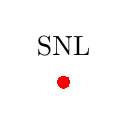
\begin{tikzpicture}

\begin{axis}[%
width=0.96731\figurewidth,
height=\figureheight,
at={(0\figurewidth,0\figureheight)},
scale only axis,
unbounded coords=jump,
every outer x axis line/.append style={black},
every x tick label/.append style={font=\color{black}},
xtick={0,0.1},
xmin=-0.00576036866359447,
xmax=0.102534562211982,
xlabel={freq},
every outer y axis line/.append style={black},
every y tick label/.append style={font=\color{black}},
ymin=-341.742848099994,
ymax=18.7034306519713,
ylabel={Amplitude},
title={SNL},
axis x line*=bottom,
axis y line*=left
]
\addplot [color=blue,only marks,mark=o,mark options={solid},forget plot]
  table[row sep=crcr]{%
0.000244140625	8.55350673954086\\
0.00048828125	8.55590581262265\\
0.000732421875	8.56397495782221\\
0.0009765625	8.56636903193436\\
0.001220703125	8.55225563128596\\
0.00146484375	8.56189590780002\\
0.001708984375	8.55379296549472\\
0.001953125	8.55120958421702\\
0.002197265625	8.56455148277672\\
0.00244140625	8.55931021686109\\
0.002685546875	8.55485500239587\\
0.0029296875	8.5604280071118\\
0.003173828125	8.54849415831177\\
0.00341796875	8.56339717713888\\
0.003662109375	8.56241192542848\\
0.00390625	8.55807509740657\\
0.004150390625	8.55720944514985\\
0.00439453125	8.55588796719661\\
0.004638671875	8.5646038987087\\
0.0048828125	8.56654164263676\\
0.005126953125	8.55105702891905\\
0.00537109375	8.55073693326733\\
0.005615234375	8.55950799849091\\
0.005859375	8.55975029145452\\
0.006103515625	8.56397635797498\\
0.00634765625	8.56073412985819\\
0.006591796875	8.55857627152284\\
0.0068359375	8.55464225471752\\
0.007080078125	8.55255738165187\\
0.00732421875	8.55954649259326\\
0.007568359375	8.55628452600342\\
0.0078125	8.55706685514207\\
0.008056640625	8.56142095557459\\
0.00830078125	8.55252209256406\\
0.008544921875	8.5502466415644\\
0.0087890625	8.55282902071326\\
0.009033203125	8.55437797072062\\
0.00927734375	8.56067050378067\\
0.009521484375	8.56029676269497\\
0.009765625	8.56849189118986\\
0.010009765625	8.55737624507816\\
0.01025390625	8.5665969029742\\
0.010498046875	8.56075305495699\\
0.0107421875	8.56163074961978\\
0.010986328125	8.56096172359332\\
0.01123046875	8.55497702388669\\
0.011474609375	8.55561679532605\\
0.01171875	8.56238315585193\\
0.011962890625	8.54905384787128\\
0.01220703125	8.55233340153046\\
0.012451171875	8.55774842522396\\
0.0126953125	8.55705257590961\\
0.012939453125	8.5545293027846\\
0.01318359375	8.55478151860007\\
0.013427734375	8.56131976515445\\
0.013671875	8.56518187191921\\
0.013916015625	8.56052439279443\\
0.01416015625	8.56330057791422\\
0.014404296875	8.56297272964957\\
0.0146484375	8.55221228993105\\
0.014892578125	8.55553382998113\\
0.01513671875	8.5550881442677\\
0.015380859375	8.56503732196256\\
0.015625	8.56256741581211\\
0.015869140625	8.55278916296726\\
0.01611328125	8.55566384659403\\
0.016357421875	8.55762263841655\\
0.0166015625	8.56318117882842\\
0.016845703125	8.55640062467546\\
0.01708984375	8.5544253076211\\
0.017333984375	8.55913796279862\\
0.017578125	8.56306978167004\\
0.017822265625	8.55798752255589\\
0.01806640625	8.56569345572058\\
0.018310546875	8.5457663480251\\
0.0185546875	8.5537986858954\\
0.018798828125	8.55861503985682\\
0.01904296875	8.56057918638953\\
0.019287109375	8.56083452273276\\
0.01953125	8.56054581584948\\
0.019775390625	8.56006425292429\\
0.02001953125	8.56309373667608\\
0.020263671875	8.56703195285968\\
0.0205078125	8.55429108198058\\
0.020751953125	8.55792472584079\\
0.02099609375	8.56439437997847\\
0.021240234375	8.56426573433316\\
0.021484375	8.55429863237089\\
0.021728515625	8.55346134233082\\
0.02197265625	8.56556163721547\\
0.022216796875	8.56394283499668\\
0.0224609375	8.55544477824645\\
0.022705078125	8.56099575968295\\
0.02294921875	8.56665275287457\\
0.023193359375	8.5655583271548\\
0.0234375	8.567152132096\\
0.023681640625	8.56174955260116\\
0.02392578125	8.5627452839795\\
0.024169921875	8.56114241468146\\
0.0244140625	8.56490250407217\\
0.024658203125	8.55166990438323\\
0.02490234375	8.55848361785735\\
0.025146484375	-308.226004638934\\
0.025390625	-319.791010966599\\
0.025634765625	-304.521000032424\\
0.02587890625	-306.612649060923\\
0.026123046875	-304.480069463168\\
0.0263671875	-307.8319312525\\
0.026611328125	-309.179120711577\\
0.02685546875	-304.092854040447\\
0.027099609375	-310.957131048929\\
0.02734375	-315.052422752546\\
0.027587890625	-313.190176923547\\
0.02783203125	-321.625587606638\\
0.028076171875	-307.825399879466\\
0.0283203125	-309.729463556496\\
0.028564453125	-316.362573414479\\
0.02880859375	-317.497285329506\\
0.029052734375	-311.264397643858\\
0.029296875	-322.766233391013\\
0.029541015625	-313.303595914686\\
0.02978515625	-307.245059067252\\
0.030029296875	-315.032004437237\\
0.0302734375	-312.920743887868\\
0.030517578125	-313.898038475724\\
0.03076171875	-320.948843592125\\
0.031005859375	-313.635313564157\\
0.03125	-324.506337705425\\
0.031494140625	-311.077101637184\\
0.03173828125	-317.147475198062\\
0.031982421875	-313.575348931025\\
0.0322265625	-329.082101868917\\
0.032470703125	-321.786322260458\\
0.03271484375	-318.766966168387\\
0.032958984375	-314.342571051545\\
0.033203125	-317.399338009446\\
0.033447265625	-309.799526781294\\
0.03369140625	-313.463452027975\\
0.033935546875	-316.9223827019\\
0.0341796875	-315.663816472031\\
0.034423828125	-309.218913386684\\
0.03466796875	-309.533865237357\\
0.034912109375	-309.953262560731\\
0.03515625	-314.866414247159\\
0.035400390625	-316.98069248758\\
0.03564453125	-311.608701300114\\
0.035888671875	-314.963708362321\\
0.0361328125	-314.835534005254\\
0.036376953125	-314.878717794919\\
0.03662109375	-316.508046952085\\
0.036865234375	-315.703496259141\\
0.037109375	-333.028120172213\\
0.037353515625	-311.669404943713\\
0.03759765625	-312.10209536046\\
0.037841796875	-325.1123953171\\
0.0380859375	-319.09179540382\\
0.038330078125	-307.050595577261\\
0.03857421875	-306.787306190037\\
0.038818359375	-304.581610882266\\
0.0390625	-312.807906103317\\
0.039306640625	-319.09179540382\\
0.03955078125	-307.952361880752\\
0.039794921875	-303.40977816315\\
0.0400390625	-310.060895533901\\
0.040283203125	-313.07119549054\\
0.04052734375	-307.050595577261\\
0.040771484375	-319.09179540382\\
nan	nan\\
0.041259765625	-321.960238249866\\
0.04150390625	-307.050595577261\\
0.041748046875	-305.1123953171\\
0.0419921875	-307.046356489741\\
0.042236328125	-309.51931520803\\
0.04248046875	-306.08149544718\\
0.042724609375	-312.807906103317\\
0.04296875	-319.09179540382\\
0.043212890625	-309.549370309427\\
0.04345703125	-313.07119549054\\
nan	nan\\
0.0439453125	-309.549370309427\\
0.044189453125	-313.07119549054\\
0.04443359375	-319.09179540382\\
0.044677734375	-310.332144379921\\
0.044921875	-319.09179540382\\
0.045166015625	-310.305141527215\\
0.04541015625	-331.132995230379\\
0.045654296875	-312.807906103317\\
0.0458984375	-313.07119549054\\
0.046142578125	-325.1123953171\\
0.04638671875	-308.461277946349\\
0.046630859375	-306.08149544718\\
0.046875	-317.092200819668\\
0.047119140625	-314.309096744798\\
0.04736328125	-321.356406930634\\
0.047607421875	-317.903818918079\\
0.0478515625	-313.667597737138\\
0.048095703125	-310.82262947639\\
0.04833984375	-316.491364206984\\
0.048583984375	-310.647942535076\\
0.048828125	-306.757082163626\\
0.049072265625	-312.709924768508\\
0.04931640625	-315.739932042868\\
0.049560546875	-310.356848202837\\
0.0498046875	-328.272067292964\\
0.050048828125	-308.115450303511\\
0.05029296875	-312.000752642666\\
0.050537109375	-312.98445977118\\
0.05078125	-309.215881428334\\
0.051025390625	-311.349946507933\\
0.05126953125	-318.601317929511\\
0.051513671875	-323.824538625492\\
0.0517578125	-318.536529472743\\
0.052001953125	-313.807776033038\\
0.05224609375	-311.061051581723\\
0.052490234375	-312.40511923358\\
0.052734375	-315.931240876393\\
0.052978515625	-309.663005373483\\
0.05322265625	-308.669976177031\\
0.053466796875	-316.707826333763\\
0.0537109375	-318.800437537408\\
0.053955078125	-307.69025491516\\
0.05419921875	-310.956796117199\\
0.054443359375	-306.740720378909\\
0.0546875	-316.451017693241\\
0.054931640625	-306.760647066199\\
0.05517578125	-311.135393463317\\
0.055419921875	-312.461141463871\\
0.0556640625	-322.172783334109\\
0.055908203125	-310.459926007421\\
0.05615234375	-315.452107961114\\
0.056396484375	-310.160511725858\\
0.056640625	-326.323909894344\\
0.056884765625	-320.304424062247\\
0.05712890625	-324.586922598025\\
0.057373046875	-309.540577707701\\
0.0576171875	-312.313938518167\\
0.057861328125	-312.840210561578\\
0.05810546875	-312.482913128453\\
0.058349609375	-315.215058842567\\
0.05859375	-336.988512817801\\
0.058837890625	-313.013174465972\\
0.05908203125	-315.323043020818\\
0.059326171875	-329.836252107513\\
0.0595703125	-312.843207448756\\
0.059814453125	-315.500599705993\\
0.06005859375	-315.319256400951\\
0.060302734375	-312.974847083585\\
0.060546875	-312.518467631408\\
0.060791015625	-318.795219272641\\
0.06103515625	-315.127273895056\\
0.061279296875	-319.773374288619\\
0.0615234375	-311.398958006308\\
0.061767578125	-318.961436851172\\
0.06201171875	-307.690723268649\\
0.062255859375	-324.895614369408\\
0.0625	-318.931792385811\\
0.062744140625	-313.791866877524\\
0.06298828125	-323.062745762084\\
0.063232421875	-317.81903887586\\
0.0634765625	-313.693678543766\\
0.063720703125	-316.363582784729\\
0.06396484375	-307.660423785521\\
0.064208984375	-320.448743977808\\
0.064453125	-307.775563311059\\
0.064697265625	-334.398498471074\\
0.06494140625	-307.136695260897\\
0.065185546875	-307.886206003379\\
0.0654296875	-320.379797054456\\
0.065673828125	-316.672755373253\\
0.06591796875	-316.707600294625\\
0.066162109375	-306.71095255035\\
0.06640625	-312.063969365983\\
0.066650390625	-313.673802716354\\
0.06689453125	-320.180429098946\\
0.067138671875	-318.350050033588\\
0.0673828125	-321.53331161883\\
0.067626953125	-322.8309563474\\
0.06787109375	-312.397778335051\\
0.068115234375	-323.071558841613\\
0.068359375	-313.895844989518\\
0.068603515625	-327.00752185462\\
0.06884765625	-325.002366995448\\
0.069091796875	-322.807379869818\\
0.0693359375	-319.814622780142\\
0.069580078125	-308.752440494678\\
0.06982421875	-309.743628160795\\
0.070068359375	-317.431829056473\\
0.0703125	-320.409539488055\\
0.070556640625	-316.534253529521\\
0.07080078125	-319.562225688775\\
0.071044921875	-315.993462978558\\
0.0712890625	-321.67915334561\\
0.071533203125	-311.530880633266\\
0.07177734375	-312.724790281843\\
0.072021484375	-317.255192003317\\
0.072265625	-321.179334115284\\
0.072509765625	-313.626035457864\\
0.07275390625	-308.138347532613\\
0.072998046875	-315.815782190709\\
0.0732421875	-304.88582477878\\
0.073486328125	-315.732176008029\\
0.07373046875	-309.138356601021\\
0.073974609375	-312.134487375884\\
0.07421875	-317.725606216476\\
0.074462890625	-321.180161075464\\
0.07470703125	-319.391285718548\\
0.074951171875	-319.416487184779\\
0.0751953125	-320.190695176988\\
0.075439453125	-309.073358383897\\
0.07568359375	-309.572655064409\\
0.075927734375	-305.160157421186\\
0.076171875	-310.319589742456\\
0.076416015625	-310.485335349771\\
0.07666015625	-312.732154611256\\
0.076904296875	-307.256018387709\\
0.0771484375	-306.54231483019\\
0.077392578125	-322.419528658008\\
0.07763671875	-303.675554269078\\
0.077880859375	-307.16094384377\\
0.078125	-315.766042605044\\
0.078369140625	-309.875615142341\\
0.07861328125	-313.825250288856\\
0.078857421875	-310.686589935568\\
0.0791015625	-308.799567944684\\
0.079345703125	-314.051752925036\\
0.07958984375	-312.967675460751\\
0.079833984375	-316.113741008221\\
0.080078125	-306.446558096223\\
0.080322265625	-317.680616339876\\
0.08056640625	-312.009270240773\\
0.080810546875	-332.138921569402\\
0.0810546875	-316.620258677461\\
0.081298828125	-312.210576892494\\
0.08154296875	-316.92643825769\\
0.081787109375	-312.999598968908\\
0.08203125	-318.034846617694\\
0.082275390625	-323.586438499606\\
0.08251953125	-314.711938314365\\
0.082763671875	-312.591697646458\\
0.0830078125	-308.39775430044\\
0.083251953125	-314.19491121222\\
0.08349609375	-316.578282611462\\
0.083740234375	-314.150099326794\\
0.083984375	-314.926129298843\\
0.084228515625	-320.486704689421\\
0.08447265625	-313.451481513589\\
0.084716796875	-335.17953782616\\
0.0849609375	-311.901448726575\\
0.085205078125	-315.057025593391\\
0.08544921875	-316.492716371414\\
0.085693359375	-315.942145984147\\
0.0859375	-311.859173724187\\
0.086181640625	-315.680841135169\\
0.08642578125	-315.420720302379\\
0.086669921875	-315.758862828999\\
0.0869140625	-313.475333691849\\
0.087158203125	-310.866189518187\\
0.08740234375	-309.825173670595\\
0.087646484375	-309.86463328752\\
0.087890625	-326.196320607452\\
0.088134765625	-317.886139054003\\
0.08837890625	-311.619469291405\\
0.088623046875	-315.992530134719\\
0.0888671875	-319.875286781456\\
0.089111328125	-314.735886304747\\
0.08935546875	-324.461014258747\\
0.089599609375	-310.505667324923\\
0.08984375	-309.053101887918\\
0.090087890625	-325.202227300099\\
0.09033203125	-310.257201565836\\
0.090576171875	-312.678656280782\\
0.0908203125	-316.068258327069\\
0.091064453125	-316.900569642096\\
0.09130859375	-312.462538250446\\
0.091552734375	-307.347501452076\\
0.091796875	-310.151639853829\\
0.092041015625	-315.211478050516\\
0.09228515625	-311.661551495165\\
0.092529296875	-307.072693014169\\
0.0927734375	-328.766624219249\\
0.093017578125	-310.283431177704\\
0.09326171875	-323.209500876295\\
0.093505859375	-321.892892522477\\
0.09375	-321.560561716326\\
0.093994140625	-310.762804527458\\
0.09423828125	-312.298728339527\\
0.094482421875	-324.290593161113\\
0.0947265625	-318.381109496037\\
0.094970703125	-314.594802414218\\
0.09521484375	-312.663287040882\\
0.095458984375	-315.652530826615\\
0.095703125	-318.844206065898\\
0.095947265625	-317.440145436689\\
0.09619140625	-312.836613778798\\
0.096435546875	-307.480913250724\\
0.0966796875	-305.157635604416\\
0.096923828125	-308.801095163579\\
0.09716796875	-308.347951657188\\
0.097412109375	-308.471912945222\\
0.09765625	-314.405967673374\\
0.097900390625	-323.971038518812\\
0.09814453125	-314.64787179143\\
0.098388671875	-314.811459444794\\
0.0986328125	-315.644926948598\\
0.098876953125	-317.762056316609\\
0.09912109375	-322.689988178272\\
0.099365234375	-315.23465576589\\
0.099609375	-321.019621219149\\
0.099853515625	-319.456522193474\\
0.10009765625	-310.642115249032\\
0.100341796875	-310.656527883585\\
0.1005859375	-311.888847698003\\
0.100830078125	-316.810485666217\\
0.10107421875	-315.496722769499\\
0.101318359375	-317.780116552719\\
0.1015625	-311.173010026333\\
0.101806640625	-310.606470771608\\
0.10205078125	-310.20666045155\\
0.102294921875	-313.66523356021\\
0.1025390625	-314.83801659319\\
};
\addplot [color=black!50!green,only marks,mark=*,mark options={solid},forget plot]
  table[row sep=crcr]{%
0.000244140625	8.55350673954086\\
0.00048828125	8.55590581262265\\
0.000732421875	8.56397495782221\\
0.0009765625	8.56636903193436\\
0.001220703125	8.55225563128596\\
0.00146484375	8.56189590780002\\
0.001708984375	8.55379296549472\\
0.001953125	8.55120958421702\\
0.002197265625	8.56455148277672\\
0.00244140625	8.55931021686109\\
0.002685546875	8.55485500239587\\
0.0029296875	8.5604280071118\\
0.003173828125	8.54849415831177\\
0.00341796875	8.56339717713888\\
0.003662109375	8.56241192542853\\
0.00390625	8.55807509740657\\
0.004150390625	8.55720944514985\\
0.00439453125	8.55588796719661\\
0.004638671875	8.5646038987087\\
0.0048828125	8.56654164263676\\
0.005126953125	8.55105702891905\\
0.00537109375	8.55073693326733\\
0.005615234375	8.55950799849091\\
0.005859375	8.55975029145452\\
0.006103515625	8.56397635797498\\
0.00634765625	8.56073412985819\\
0.006591796875	8.55857627152284\\
0.0068359375	8.55464225471752\\
0.007080078125	8.55255738165187\\
0.00732421875	8.55954649259326\\
0.007568359375	8.55628452600342\\
0.0078125	8.55706685514207\\
0.008056640625	8.56142095557459\\
0.00830078125	8.55252209256406\\
0.008544921875	8.5502466415644\\
0.0087890625	8.55282902071326\\
0.009033203125	8.55437797072062\\
0.00927734375	8.56067050378067\\
0.009521484375	8.56029676269497\\
0.009765625	8.56849189118986\\
0.010009765625	8.55737624507816\\
0.01025390625	8.5665969029742\\
0.010498046875	8.56075305495699\\
0.0107421875	8.56163074961978\\
0.010986328125	8.56096172359332\\
0.01123046875	8.55497702388669\\
0.011474609375	8.55561679532605\\
0.01171875	8.56238315585193\\
0.011962890625	8.54905384787128\\
0.01220703125	8.55233340153046\\
0.012451171875	8.55774842522396\\
0.0126953125	8.55705257590961\\
0.012939453125	8.55452930278466\\
0.01318359375	8.55478151860007\\
0.013427734375	8.56131976515445\\
0.013671875	8.56518187191921\\
0.013916015625	8.56052439279443\\
0.01416015625	8.56330057791422\\
0.014404296875	8.56297272964957\\
0.0146484375	8.55221228993105\\
0.014892578125	8.55553382998113\\
0.01513671875	8.5550881442677\\
0.015380859375	8.56503732196256\\
0.015625	8.56256741581211\\
0.015869140625	8.55278916296726\\
0.01611328125	8.55566384659403\\
0.016357421875	8.55762263841655\\
0.0166015625	8.56318117882842\\
0.016845703125	8.55640062467546\\
0.01708984375	8.5544253076211\\
0.017333984375	8.55913796279862\\
0.017578125	8.56306978167004\\
0.017822265625	8.55798752255589\\
0.01806640625	8.56569345572058\\
0.018310546875	8.5457663480251\\
0.0185546875	8.5537986858954\\
0.018798828125	8.55861503985682\\
0.01904296875	8.56057918638953\\
0.019287109375	8.56083452273276\\
0.01953125	8.56054581584948\\
0.019775390625	8.56006425292429\\
0.02001953125	8.56309373667608\\
0.020263671875	8.56703195285968\\
0.0205078125	8.55429108198058\\
0.020751953125	8.55792472584079\\
0.02099609375	8.56439437997847\\
0.021240234375	8.56426573433316\\
0.021484375	8.55429863237089\\
0.021728515625	8.55346134233082\\
0.02197265625	8.56556163721547\\
0.022216796875	8.56394283499668\\
0.0224609375	8.55544477824645\\
0.022705078125	8.56099575968295\\
0.02294921875	8.56665275287457\\
0.023193359375	8.5655583271548\\
0.0234375	8.567152132096\\
0.023681640625	8.56174955260116\\
0.02392578125	8.5627452839795\\
0.024169921875	8.56114241468146\\
0.0244140625	8.56490250407217\\
0.024658203125	8.55166990438323\\
0.02490234375	8.55848361785735\\
0.025146484375	-311.434042098426\\
0.025390625	-314.490094583876\\
0.025634765625	-307.914677175221\\
0.02587890625	-310.402585291898\\
0.026123046875	-305.820917606603\\
0.0263671875	-310.776027472262\\
0.026611328125	-310.295025328976\\
0.02685546875	-303.124578000092\\
0.027099609375	-331.370261575289\\
0.02734375	-319.374831017504\\
0.027587890625	-311.883797126073\\
0.02783203125	-312.807831151416\\
0.028076171875	-306.926985447065\\
0.0283203125	-311.069985741456\\
0.028564453125	-324.721896131877\\
0.02880859375	-317.593504056448\\
0.029052734375	-312.504426505466\\
0.029296875	-323.515478736182\\
0.029541015625	-313.241094758796\\
0.02978515625	-304.740784771739\\
0.030029296875	-314.887190355334\\
0.0302734375	-313.928837858823\\
0.030517578125	-309.291922301106\\
0.03076171875	-314.775365663777\\
0.031005859375	-314.547659394721\\
0.03125	-313.384379963109\\
0.031494140625	-310.979749966906\\
0.03173828125	-314.704012924397\\
0.031982421875	-312.185980407525\\
0.0322265625	-327.913843779055\\
0.032470703125	-319.245826337884\\
0.03271484375	-314.063055566547\\
0.032958984375	-317.007456278745\\
0.033203125	-318.055368240584\\
0.033447265625	-310.510242884779\\
0.03369140625	-315.76208485266\\
0.033935546875	-314.180794347219\\
0.0341796875	-315.702569656517\\
0.034423828125	-316.068584853556\\
0.03466796875	-309.734440502876\\
0.034912109375	-311.428993182671\\
0.03515625	-317.950814791699\\
0.035400390625	-321.144430481685\\
0.03564453125	-316.051915090527\\
0.035888671875	-318.057751791464\\
0.0361328125	-314.159646988173\\
0.036376953125	-309.885603354816\\
0.03662109375	-317.770482765553\\
0.036865234375	-312.51772762208\\
0.037109375	-338.814797407462\\
0.037353515625	-311.343477804895\\
0.03759765625	-312.10209536046\\
0.037841796875	-303.40977816315\\
nan	nan\\
0.038330078125	-313.07119549054\\
0.03857421875	-313.07119549054\\
0.038818359375	-302.963956836623\\
0.0390625	-319.09179540382\\
0.039306640625	-311.132995230379\\
0.03955078125	-307.952361880752\\
0.039794921875	-303.40977816315\\
0.0400390625	-313.07119549054\\
0.040283203125	-306.08149544718\\
0.04052734375	-313.07119549054\\
0.040771484375	-306.983261750671\\
0.041015625	-313.07119549054\\
0.041259765625	-306.960809133134\\
0.04150390625	-312.10209536046\\
0.041748046875	-314.231034430094\\
0.0419921875	-320.251634343374\\
0.042236328125	-313.631769962545\\
0.04248046875	-312.666531944608\\
0.042724609375	-321.590570135986\\
0.04296875	-312.10209536046\\
0.043212890625	-307.050595577261\\
0.04345703125	-319.09179540382\\
0.043701171875	-307.050595577261\\
0.0439453125	-312.10209536046\\
0.044189453125	-319.09179540382\\
0.04443359375	-307.050595577261\\
0.044677734375	-309.250743503326\\
0.044921875	-313.07119549054\\
0.045166015625	-313.07119549054\\
0.04541015625	-307.050595577261\\
0.045654296875	-312.10209536046\\
0.0458984375	-316.08149544718\\
0.046142578125	-319.09179540382\\
0.04638671875	-312.048145041593\\
0.046630859375	-305.1123953171\\
0.046875	-315.366469559518\\
0.047119140625	-312.793912036776\\
0.04736328125	-313.288740124089\\
0.047607421875	-310.149488868823\\
0.0478515625	-312.595135042771\\
0.048095703125	-320.389186275481\\
0.04833984375	-313.707974811996\\
0.048583984375	-313.067282028164\\
0.048828125	-316.1594029674\\
0.049072265625	-314.472888470115\\
0.04931640625	-326.274841064839\\
0.049560546875	-309.083352692195\\
0.0498046875	-316.806989671526\\
0.050048828125	-310.08635710952\\
0.05029296875	-325.662292165697\\
0.050537109375	-310.971035034401\\
0.05078125	-311.115774424603\\
0.051025390625	-305.600587508883\\
0.05126953125	-312.033825075313\\
0.051513671875	-311.249338161196\\
0.0517578125	-312.664396633593\\
0.052001953125	-317.244886282587\\
0.05224609375	-314.505901797571\\
0.052490234375	-314.50080595656\\
0.052734375	-310.715995429571\\
0.052978515625	-308.002955977851\\
0.05322265625	-309.107950947251\\
0.053466796875	-310.91569968443\\
0.0537109375	-316.352667574072\\
0.053955078125	-309.454018349658\\
0.05419921875	-309.650861310353\\
0.054443359375	-306.834237296985\\
0.0546875	-312.595903655027\\
0.054931640625	-306.410043433748\\
0.05517578125	-322.266986845565\\
0.055419921875	-308.843764938902\\
0.0556640625	-313.072539644043\\
0.055908203125	-313.258658706593\\
0.05615234375	-315.740793512492\\
0.056396484375	-315.030040593643\\
0.056640625	-319.813410710305\\
0.056884765625	-326.604944704811\\
0.05712890625	-311.255697191232\\
0.057373046875	-308.72557183156\\
0.0576171875	-309.609413829263\\
0.057861328125	-312.845126087464\\
0.05810546875	-310.883087887949\\
0.058349609375	-313.885729915342\\
0.05859375	-318.345382901231\\
0.058837890625	-316.922872398027\\
0.05908203125	-311.79585616319\\
0.059326171875	-318.85566895259\\
0.0595703125	-308.842652006088\\
0.059814453125	-316.487237628011\\
0.06005859375	-311.134802118575\\
0.060302734375	-311.787562483555\\
0.060546875	-314.024395553648\\
0.060791015625	-314.640190205907\\
0.06103515625	-321.610091397782\\
0.061279296875	-323.315789900086\\
0.0615234375	-307.743569889479\\
0.061767578125	-317.89386780728\\
0.06201171875	-307.988136426891\\
0.062255859375	-318.692739414247\\
0.0625	-315.930750238395\\
0.062744140625	-313.154312407504\\
0.06298828125	-321.80365117871\\
0.063232421875	-313.913176472859\\
0.0634765625	-324.63467229635\\
0.063720703125	-312.192376100965\\
0.06396484375	-308.568649259054\\
0.064208984375	-312.875152480487\\
0.064453125	-316.016527285703\\
0.064697265625	-329.875321628739\\
0.06494140625	-306.302754184229\\
0.065185546875	-313.395388099714\\
0.0654296875	-325.657272980574\\
0.065673828125	-313.161682921412\\
0.06591796875	-315.992798413913\\
0.066162109375	-311.844672835937\\
0.06640625	-310.552064414699\\
0.066650390625	-311.59376167361\\
0.06689453125	-328.881931898862\\
0.067138671875	-311.783335917736\\
0.0673828125	-317.069199568617\\
0.067626953125	-310.640527598589\\
0.06787109375	-317.39888226431\\
0.068115234375	-323.022401217161\\
0.068359375	-315.631737447864\\
0.068603515625	-315.462108391055\\
0.06884765625	-312.235936619237\\
0.069091796875	-313.567515965765\\
0.0693359375	-311.313058655379\\
0.069580078125	-315.774838053075\\
0.06982421875	-314.359889224812\\
0.070068359375	-315.185888863108\\
0.0703125	-318.490355036383\\
0.070556640625	-320.682449765102\\
0.07080078125	-313.962018493226\\
0.071044921875	-322.979328747262\\
0.0712890625	-324.46515937538\\
0.071533203125	-317.615462471003\\
0.07177734375	-315.041771391868\\
0.072021484375	-313.953112631592\\
0.072265625	-313.443070265363\\
0.072509765625	-321.776035685164\\
0.07275390625	-307.993211235656\\
0.072998046875	-307.464259969975\\
0.0732421875	-304.757502780489\\
0.073486328125	-319.359315206172\\
0.07373046875	-307.580494662296\\
0.073974609375	-315.656797056505\\
0.07421875	-315.100719924605\\
0.074462890625	-321.46743763639\\
0.07470703125	-318.585089186169\\
0.074951171875	-311.496914157447\\
0.0751953125	-311.568659514091\\
0.075439453125	-310.595373472295\\
0.07568359375	-307.818036887975\\
0.075927734375	-305.445562699589\\
0.076171875	-308.160544881159\\
0.076416015625	-306.969262069444\\
0.07666015625	-311.752702219559\\
0.076904296875	-308.956834494186\\
0.0771484375	-306.615978067439\\
0.077392578125	-324.424919635037\\
0.07763671875	-303.480295123795\\
0.077880859375	-309.054197897663\\
0.078125	-312.445652839854\\
0.078369140625	-305.875456088654\\
0.07861328125	-314.873718611816\\
0.078857421875	-326.004864547673\\
0.0791015625	-314.599098426629\\
0.079345703125	-322.185551801421\\
0.07958984375	-310.326286738974\\
0.079833984375	-313.987312657791\\
0.080078125	-310.852651509642\\
0.080322265625	-318.906913790397\\
0.08056640625	-311.24026107243\\
0.080810546875	-323.34977917779\\
0.0810546875	-312.992556765616\\
0.081298828125	-311.902418039449\\
0.08154296875	-316.21089846869\\
0.081787109375	-322.224978512637\\
0.08203125	-315.141720176462\\
0.082275390625	-311.435860967037\\
0.08251953125	-315.59940082997\\
0.082763671875	-329.529847181985\\
0.0830078125	-310.553977919194\\
0.083251953125	-328.242482355774\\
0.08349609375	-311.275297840138\\
0.083740234375	-312.454955559295\\
0.083984375	-314.370496545016\\
0.084228515625	-310.03115963276\\
0.08447265625	-320.979089634108\\
0.084716796875	-313.838607403199\\
0.0849609375	-312.727971966443\\
0.085205078125	-313.325467585706\\
0.08544921875	-312.952058588525\\
0.085693359375	-311.844842607609\\
0.0859375	-312.796189677957\\
0.086181640625	-311.277927127949\\
0.08642578125	-317.308937858612\\
0.086669921875	-314.079291874863\\
0.0869140625	-312.668988950907\\
0.087158203125	-310.04623802175\\
0.08740234375	-312.606603706738\\
0.087646484375	-309.783637697212\\
0.087890625	-312.947166337383\\
0.088134765625	-312.601668655559\\
0.08837890625	-316.87859664067\\
0.088623046875	-314.598293165497\\
0.0888671875	-320.209436599307\\
0.089111328125	-309.579789646003\\
0.08935546875	-325.238484548565\\
0.089599609375	-313.811705438549\\
0.08984375	-308.125812552027\\
0.090087890625	-313.12384861152\\
0.09033203125	-319.978367829896\\
0.090576171875	-306.574500925363\\
0.0908203125	-313.880037383452\\
0.091064453125	-313.226671520762\\
0.09130859375	-310.797982205575\\
0.091552734375	-312.307457640728\\
0.091796875	-310.603068168081\\
0.092041015625	-309.439920603244\\
0.09228515625	-309.199116430382\\
0.092529296875	-307.843907279366\\
0.0927734375	-318.467091077015\\
0.093017578125	-314.721270510218\\
0.09326171875	-322.633693723727\\
0.093505859375	-315.308324748557\\
0.09375	-327.206543956555\\
0.093994140625	-313.015939428964\\
0.09423828125	-313.925150984725\\
0.094482421875	-314.298752421966\\
0.0947265625	-315.08458234981\\
0.094970703125	-314.389696853644\\
0.09521484375	-309.892457547149\\
0.095458984375	-311.864656535231\\
0.095703125	-319.316289680754\\
0.095947265625	-335.785067216553\\
0.09619140625	-314.466963588431\\
0.096435546875	-307.315979381025\\
0.0966796875	-306.96439185573\\
0.096923828125	-309.512461685551\\
0.09716796875	-306.978103385801\\
0.097412109375	-306.509106120431\\
0.09765625	-311.072011474133\\
0.097900390625	-320.206131650253\\
0.09814453125	-316.043434461472\\
0.098388671875	-311.653965320777\\
0.0986328125	-315.18272799906\\
0.098876953125	-312.264914527244\\
0.09912109375	-314.089117630782\\
0.099365234375	-316.845088418086\\
0.099609375	-319.009920223629\\
0.099853515625	-311.511982926293\\
0.10009765625	-114.455922235248\\
0.100341796875	-116.269138084271\\
0.1005859375	-118.271618333062\\
0.100830078125	-112.04572736784\\
0.10107421875	-110.846359228952\\
0.101318359375	-113.049550065086\\
0.1015625	-125.93561598655\\
0.101806640625	-120.611669176763\\
0.10205078125	-117.279319025283\\
0.102294921875	-119.054236445743\\
0.1025390625	-125.57979828686\\
};
\addplot [color=red,only marks,mark=*,mark options={solid},forget plot]
  table[row sep=crcr]{%
0.000244140625	8.56068421913295\\
0.00048828125	8.55989436404724\\
0.000732421875	8.5610168209916\\
0.0009765625	8.58343323829604\\
0.001220703125	8.57567604133959\\
0.00146484375	8.55860783133312\\
0.001708984375	8.57963205139197\\
0.001953125	8.56719843392887\\
0.002197265625	8.55708425649038\\
0.00244140625	8.5541522800587\\
0.002685546875	8.5564824150224\\
0.0029296875	8.54377733065292\\
0.003173828125	8.54721210675177\\
0.00341796875	8.54863324407188\\
0.003662109375	8.57287974902425\\
0.00390625	8.55847170288769\\
0.004150390625	8.57169157216799\\
0.00439453125	8.56800921052002\\
0.004638671875	8.5496510302122\\
0.0048828125	8.55836129510737\\
0.005126953125	8.55119191146099\\
0.00537109375	8.55273173614398\\
0.005615234375	8.5690984997712\\
0.005859375	8.57696160544907\\
0.006103515625	8.5925530069693\\
0.00634765625	8.55891033649795\\
0.006591796875	8.5544887072939\\
0.0068359375	8.57854436555454\\
0.007080078125	8.56846077544321\\
0.00732421875	8.55760176674966\\
0.007568359375	8.56497471314322\\
0.0078125	8.57120185795685\\
0.008056640625	8.57744319126618\\
0.00830078125	8.55263500065536\\
0.008544921875	8.54903405471765\\
0.0087890625	8.56339400254473\\
0.009033203125	8.5597628365058\\
0.00927734375	8.54859992427276\\
0.009521484375	8.56631850949179\\
0.009765625	8.57525464913709\\
0.010009765625	8.58436122826834\\
0.01025390625	8.56640483486916\\
0.010498046875	8.57235844647278\\
0.0107421875	8.56560698321067\\
0.010986328125	8.55201640136215\\
0.01123046875	8.56189308761185\\
0.011474609375	8.56482219905655\\
0.01171875	8.56661152753446\\
0.011962890625	8.55555243107329\\
0.01220703125	8.55398091512694\\
0.012451171875	8.57578355698155\\
0.0126953125	8.55183694843817\\
0.012939453125	8.5863892602743\\
0.01318359375	8.56038357911569\\
0.013427734375	8.55051656399087\\
0.013671875	8.5683718812885\\
0.013916015625	8.56674256485388\\
0.01416015625	8.56518723200043\\
0.014404296875	8.55056361518263\\
0.0146484375	8.54646349317977\\
0.014892578125	8.53738947895999\\
0.01513671875	8.57025614543943\\
0.015380859375	8.55585872598471\\
0.015625	8.58010163674169\\
0.015869140625	8.56298894396559\\
0.01611328125	8.5718311810877\\
0.016357421875	8.55206745467638\\
0.0166015625	8.55247527940088\\
0.016845703125	8.57292307673532\\
0.01708984375	8.5450288481984\\
0.017333984375	8.5530686437657\\
0.017578125	8.57804722260119\\
0.017822265625	8.56822274949161\\
0.01806640625	8.55584060777051\\
0.018310546875	8.54488942190795\\
0.0185546875	8.54650667736809\\
0.018798828125	8.55812182486653\\
0.01904296875	8.56926269524621\\
0.019287109375	8.55804113211667\\
0.01953125	8.5681120940402\\
0.019775390625	8.5681484840531\\
0.02001953125	8.57742623008932\\
0.020263671875	8.59692815038045\\
0.0205078125	8.59128051906623\\
0.020751953125	8.55940477791711\\
0.02099609375	8.55196634372851\\
0.021240234375	8.56098933636531\\
0.021484375	8.57273202164657\\
0.021728515625	8.54916134005396\\
0.02197265625	8.57331799597762\\
0.022216796875	8.5435596600712\\
0.0224609375	8.55433150511357\\
0.022705078125	8.56104034295299\\
0.02294921875	8.55472841035845\\
0.023193359375	8.56582609376892\\
0.0234375	8.55668851261186\\
0.023681640625	8.56106355042567\\
0.02392578125	8.58783036903822\\
0.024169921875	8.57100590864377\\
0.0244140625	8.55071615016385\\
0.024658203125	8.56650580296241\\
0.02490234375	8.57097995403296\\
0.025146484375	-50.526364315644\\
0.025390625	-53.5852070491386\\
0.025634765625	-61.0502888078273\\
0.02587890625	-50.4811533966098\\
0.026123046875	-48.6916579447315\\
0.0263671875	-47.138495698973\\
0.026611328125	-47.6512087630425\\
0.02685546875	-51.30563719202\\
0.027099609375	-47.1539834049827\\
0.02734375	-48.0404041921871\\
0.027587890625	-60.2270657560048\\
0.02783203125	-44.6207636420738\\
0.028076171875	-60.2243855642417\\
0.0283203125	-45.0886932018596\\
0.028564453125	-47.8980946041339\\
0.02880859375	-54.875725122792\\
0.029052734375	-47.0835243131718\\
0.029296875	-49.7027970361223\\
0.029541015625	-49.3343478372664\\
0.02978515625	-46.4845290281141\\
0.030029296875	-45.9057948860622\\
0.0302734375	-50.1561765487371\\
0.030517578125	-50.3133203703524\\
0.03076171875	-53.8066810499145\\
0.031005859375	-55.3409529317042\\
0.03125	-63.671502044984\\
0.031494140625	-60.2485681264712\\
0.03173828125	-52.9135565294425\\
0.031982421875	-56.8716630353203\\
0.0322265625	-49.5185028567475\\
0.032470703125	-46.79710908956\\
0.03271484375	-47.4135476976145\\
0.032958984375	-57.1421510191409\\
0.033203125	-51.6882094057079\\
0.033447265625	-51.9629796652549\\
0.03369140625	-53.6697980243918\\
0.033935546875	-59.5059891140872\\
0.0341796875	-47.090021182266\\
0.034423828125	-56.201549612744\\
0.03466796875	-46.3208278431569\\
0.034912109375	-47.290735339629\\
0.03515625	-49.8243295393027\\
0.035400390625	-67.4780594821235\\
0.03564453125	-62.8291963714363\\
0.035888671875	-47.2757157311557\\
0.0361328125	-44.1077042735492\\
0.036376953125	-51.9735832038189\\
0.03662109375	-52.1913263255323\\
0.036865234375	-47.6460265341312\\
0.037109375	-54.2313582059771\\
0.037353515625	-49.6546251858625\\
0.03759765625	-60.2561677846587\\
0.037841796875	-51.6539151500928\\
0.0380859375	-52.2615830855407\\
0.038330078125	-50.1157505129399\\
0.03857421875	-46.5292152884461\\
0.038818359375	-50.2014864145052\\
0.0390625	-48.375895818244\\
0.039306640625	-55.0540407005511\\
0.03955078125	-51.5897670358306\\
0.039794921875	-55.8574637782111\\
0.0400390625	-47.8006517052205\\
0.040283203125	-46.979355713923\\
0.04052734375	-56.3886999498225\\
0.040771484375	-46.0717036816577\\
0.041015625	-71.6479397842029\\
0.041259765625	-61.9165630374434\\
0.04150390625	-47.1741660583106\\
0.041748046875	-46.394887209446\\
0.0419921875	-51.6222036256119\\
0.042236328125	-54.0571528179449\\
0.04248046875	-62.6693729618261\\
0.042724609375	-62.5412976722396\\
0.04296875	-53.4716956152801\\
0.043212890625	-51.0492032965981\\
0.04345703125	-49.3858099623572\\
0.043701171875	-50.7496895672438\\
0.0439453125	-46.8204011674362\\
0.044189453125	-49.3899393378599\\
0.04443359375	-59.7100823615182\\
0.044677734375	-57.7687939023943\\
0.044921875	-51.831412509948\\
0.045166015625	-54.9821841480128\\
0.04541015625	-48.6175300739258\\
0.045654296875	-54.8196638136149\\
0.0458984375	-52.0265459300872\\
0.046142578125	-49.9088399878011\\
0.04638671875	-48.3002092506644\\
0.046630859375	-50.4937019640886\\
0.046875	-59.6875729469984\\
0.047119140625	-54.4151951214414\\
0.04736328125	-70.9037560175209\\
0.047607421875	-49.6480088202566\\
0.0478515625	-45.4408960827745\\
0.048095703125	-67.5223007879412\\
0.04833984375	-53.9484401910967\\
0.048583984375	-51.3243102901018\\
0.048828125	-52.266814200481\\
0.049072265625	-50.864304185448\\
0.04931640625	-50.1735652904945\\
0.049560546875	-51.6144472174132\\
0.0498046875	-57.7976620657093\\
0.050048828125	-59.7183336449274\\
0.05029296875	-51.7005563504904\\
0.050537109375	-57.4398598771833\\
0.05078125	-57.6340540414802\\
0.051025390625	-54.648238782758\\
0.05126953125	-48.0927060933458\\
0.051513671875	-55.8105618517912\\
0.0517578125	-49.3225756621843\\
0.052001953125	-49.0770050074775\\
0.05224609375	-63.20736419152\\
0.052490234375	-52.0387632588042\\
0.052734375	-55.2118044886028\\
0.052978515625	-59.9755282580755\\
0.05322265625	-54.7413628763631\\
0.053466796875	-54.9959976702442\\
0.0537109375	-55.1072100245735\\
0.053955078125	-50.8515530108169\\
0.05419921875	-57.2062021533291\\
0.054443359375	-76.3002928191098\\
0.0546875	-54.1396158250981\\
0.054931640625	-54.7439705479071\\
0.05517578125	-50.6225450324471\\
0.055419921875	-56.8858781181184\\
0.0556640625	-63.9056330359404\\
0.055908203125	-61.422852288125\\
0.05615234375	-53.9201291825981\\
0.056396484375	-53.4201738176299\\
0.056640625	-60.6999765747273\\
0.056884765625	-59.5886799407816\\
0.05712890625	-53.4826354949033\\
0.057373046875	-59.4941099631968\\
0.0576171875	-60.0298266715381\\
0.057861328125	-52.8763018704051\\
0.05810546875	-53.3561721428506\\
0.058349609375	-56.5257284990691\\
0.05859375	-59.3526307367107\\
0.058837890625	-52.2418754058852\\
0.05908203125	-60.8116053477392\\
0.059326171875	-55.0605376304482\\
0.0595703125	-56.507101428952\\
0.059814453125	-57.0023321196496\\
0.06005859375	-56.7323973356721\\
0.060302734375	-54.4074656234837\\
0.060546875	-56.0094280526854\\
0.060791015625	-96.9297004591879\\
0.06103515625	-66.4114917781475\\
0.061279296875	-61.0731994662543\\
0.0615234375	-64.3043329285065\\
0.061767578125	-56.4931554048747\\
0.06201171875	-60.1986638862368\\
0.062255859375	-63.3481447342438\\
0.0625	-56.8965837980316\\
0.062744140625	-56.841831685529\\
0.06298828125	-68.6127855491658\\
0.063232421875	-59.7941791577663\\
0.0634765625	-67.678053676626\\
0.063720703125	-54.2776375953032\\
0.06396484375	-57.8440374681749\\
0.064208984375	-75.1026979724598\\
0.064453125	-61.5462199709253\\
0.064697265625	-60.6477305950868\\
0.06494140625	-62.4999924242486\\
0.065185546875	-61.5359695888924\\
0.0654296875	-58.8762016217273\\
0.065673828125	-62.5142585324746\\
0.06591796875	-67.6863154308723\\
0.066162109375	-62.5669494761555\\
0.06640625	-67.726200932207\\
0.066650390625	-69.6194846924168\\
0.06689453125	-68.1457269298535\\
0.067138671875	-56.2944968682881\\
0.0673828125	-58.6689988995386\\
0.067626953125	-68.4926425061476\\
0.06787109375	-56.5777099667237\\
0.068115234375	-58.0927440085499\\
0.068359375	-63.9105000549961\\
0.068603515625	-75.311226487123\\
0.06884765625	-65.1074895051394\\
0.069091796875	-67.5644849696894\\
0.0693359375	-71.8006987838883\\
0.069580078125	-64.3592277694818\\
0.06982421875	-66.6134355129895\\
0.070068359375	-66.5810444851767\\
0.0703125	-64.8084953346983\\
0.070556640625	-75.9641835300205\\
0.07080078125	-67.8085902953545\\
0.071044921875	-68.3159869217928\\
0.0712890625	-83.5740703785177\\
0.071533203125	-70.8685624530735\\
0.07177734375	-76.1330869464845\\
0.072021484375	-73.4751534576915\\
0.072265625	-69.7922941163711\\
0.072509765625	-71.2318121398146\\
0.07275390625	-72.6789624859324\\
0.072998046875	-73.0807995368866\\
0.0732421875	-70.3694149462419\\
0.073486328125	-73.2951348641648\\
0.07373046875	-76.4361732457815\\
0.073974609375	-77.7858754825421\\
0.07421875	-89.7708351538068\\
0.074462890625	-86.0362882178648\\
0.07470703125	-92.7514228879483\\
0.074951171875	-105.613886982688\\
0.0751953125	-103.555960082244\\
0.075439453125	-103.883726498963\\
0.07568359375	-107.864959373919\\
0.075927734375	-108.424232898317\\
0.076171875	-109.141147270838\\
0.076416015625	-127.047781512974\\
0.07666015625	-105.048730035649\\
0.076904296875	-103.035282662504\\
0.0771484375	-104.298045985055\\
0.077392578125	-103.926300849611\\
0.07763671875	-111.297886122932\\
0.077880859375	-108.275187502389\\
0.078125	-104.971067042275\\
0.078369140625	-102.734783352135\\
0.07861328125	-103.295940248597\\
0.078857421875	-101.33404965514\\
0.0791015625	-108.167970213839\\
0.079345703125	-102.03198664573\\
0.07958984375	-114.430552489753\\
0.079833984375	-108.121475964253\\
0.080078125	-117.866631476073\\
0.080322265625	-106.15030136725\\
0.08056640625	-105.315176518521\\
0.080810546875	-106.057627797051\\
0.0810546875	-140.289808845533\\
0.081298828125	-106.39185500335\\
0.08154296875	-110.168090545939\\
0.081787109375	-104.753429022148\\
0.08203125	-103.593156792999\\
0.082275390625	-107.590951971961\\
0.08251953125	-109.107834752624\\
0.082763671875	-118.709949949006\\
0.0830078125	-110.782347350882\\
0.083251953125	-108.207418773014\\
0.08349609375	-112.022755477553\\
0.083740234375	-110.65963977873\\
0.083984375	-106.770056376322\\
0.084228515625	-111.525396268426\\
0.08447265625	-106.885613435597\\
0.084716796875	-105.637057779463\\
0.0849609375	-114.79882330852\\
0.085205078125	-111.781044910144\\
0.08544921875	-110.511539722552\\
0.085693359375	-116.387963446881\\
0.0859375	-106.184725660629\\
0.086181640625	-112.549234303218\\
0.08642578125	-111.347146165223\\
0.086669921875	-109.095776852118\\
0.0869140625	-105.978866364876\\
0.087158203125	-116.727515840121\\
0.08740234375	-108.298177639934\\
0.087646484375	-113.856583467018\\
0.087890625	-114.962607578464\\
0.088134765625	-126.355356291148\\
0.08837890625	-112.376626418647\\
0.088623046875	-111.220415715523\\
0.0888671875	-108.406131135425\\
0.089111328125	-113.494810590982\\
0.08935546875	-108.02490855264\\
0.089599609375	-108.780587152044\\
0.08984375	-116.257160818411\\
0.090087890625	-113.942797942081\\
0.09033203125	-115.965367300753\\
0.090576171875	-115.169966921864\\
0.0908203125	-114.00312151569\\
0.091064453125	-113.278893539474\\
0.09130859375	-108.510063867913\\
0.091552734375	-107.308497876858\\
0.091796875	-113.329840298306\\
0.092041015625	-107.405887488317\\
0.09228515625	-107.656502452815\\
0.092529296875	-111.401758458743\\
0.0927734375	-119.907336243964\\
0.093017578125	-118.717605986437\\
0.09326171875	-114.037385094543\\
0.093505859375	-123.202139296521\\
0.09375	-115.420245828009\\
0.093994140625	-111.135860351579\\
0.09423828125	-110.824231396091\\
0.094482421875	-113.352585144165\\
0.0947265625	-112.009025966727\\
0.094970703125	-112.039438030648\\
0.09521484375	-119.641016342393\\
0.095458984375	-113.312589772041\\
0.095703125	-119.369921628526\\
0.095947265625	-122.121807431403\\
0.09619140625	-123.432220121643\\
0.096435546875	-117.517765404505\\
0.0966796875	-110.258032850823\\
0.096923828125	-109.372790253905\\
0.09716796875	-121.67297780285\\
0.097412109375	-109.51602611074\\
0.09765625	-111.929854426099\\
0.097900390625	-115.295221608865\\
0.09814453125	-116.093550506467\\
0.098388671875	-123.412352684054\\
0.0986328125	-113.526710990436\\
0.098876953125	-115.692384508063\\
0.09912109375	-129.076857980848\\
0.099365234375	-117.168468179306\\
0.099609375	-117.489115356756\\
0.099853515625	-117.613214669803\\
0.10009765625	-117.832183681075\\
0.100341796875	-119.515587871248\\
0.1005859375	-121.557348865947\\
0.100830078125	-115.505897528712\\
0.10107421875	-114.501340677024\\
0.101318359375	-116.896950059919\\
0.1015625	-129.363615228374\\
0.101806640625	-124.388546503922\\
0.10205078125	-120.784539301376\\
0.102294921875	-122.319636014696\\
0.1025390625	-128.400209590075\\
};
\end{axis}
\end{tikzpicture}%
		        \end{subfigure}
				\caption{Comparison of system output before and after applying ILC to the input signal in the frequency domain. Uncompensated output in red and compensated output in green.}
				\label{fig:sim_outputspec_SNL}
			\end{figure}

	Figure \ref{fig:sim_outputspec_SNL} shows the output spectrum after applying ILC for 10 iterations giving as wanted output a multisine filtered (bandwith = $0$ to $0.05 f/f_s$) trough the BLA.  The nonlinear spectral regrowth of the first iteration (red) is totally removed in the last iteration (green). Outside of the linear band, the amplitude reaches the noise levels or computer precision in the noiseless cases.
	\textbf{SHOW ILC ERROR DECREASING at each iterations}

	\subsubsection{Estimating the Digital Predistorter}

	Iterative Learning created in the previous step inputs that give a linear output to the system. A iterative algorithm is not well suited for application in predistortion. A digital predistorter is a system, not an iterative algorithm. In this step, the whole ILC algorithm  will be modelled as a nonlienar system. This is using the ILC reference outputs as input of the DPD, and the converged ILC inputs as output of the DPD.
	
	A Wiener system has been estimated for the DPD with the results plotted in figure \ref{fig:validation}.
	There is a gain with respect to non-compensated input (about $-10dB$), but the it is not as effective as the real ILC. 
	\begin{figure}
		\centering
		\setlength\figureheight{3cm} 
		\setlength\figurewidth{0.5\linewidth}
		% This file was created by matlab2tikz.
% Minimal pgfplots version: 1.3
%
%The latest updates can be retrieved from
%  http://www.mathworks.com/matlabcentral/fileexchange/22022-matlab2tikz
%where you can also make suggestions and rate matlab2tikz.
%
\definecolor{mycolor1}{rgb}{0.00000,0.75000,0.75000}%
%
\begin{tikzpicture}

\begin{axis}[%
width=0.95092\figurewidth,
height=\figureheight,
at={(0\figurewidth,0\figureheight)},
scale only axis,
every outer x axis line/.append style={black},
every x tick label/.append style={font=\color{black}},
xtick={0,0.1},
xmin=-0.00078043704474505,
xmax=0.0994128140330014,
xlabel={frequency},
every outer y axis line/.append style={black},
every y tick label/.append style={font=\color{black}},
ymin=-39.6306555863342,
ymax=53.4441366574331,
ylabel={Amplitude [db]},
title={Output Spectrum of PA},
axis x line*=bottom,
axis y line*=left
]
\addplot [color=blue,only marks,mark=*,mark options={solid},forget plot]
  table[row sep=crcr]{%
0.000244140625	50.5944577504916\\
0.00048828125	50.6397270935491\\
0.000732421875	50.6055218749084\\
0.0009765625	50.6783015377375\\
0.001220703125	50.6570361176014\\
0.00146484375	50.6643692498296\\
0.001708984375	50.6812450836532\\
0.001953125	50.6877560055908\\
0.002197265625	50.5938586216193\\
0.00244140625	50.6826178712477\\
0.002685546875	50.6001375282645\\
0.0029296875	50.6786258907181\\
0.003173828125	50.5429775229493\\
0.00341796875	50.6633177159588\\
0.003662109375	50.628988937357\\
0.00390625	50.5463983593479\\
0.004150390625	50.6234170239107\\
0.00439453125	50.5025010159446\\
0.004638671875	50.5686247447958\\
0.0048828125	50.5403681466159\\
0.005126953125	50.407406668167\\
0.00537109375	50.5942503416073\\
0.005615234375	50.4479153215626\\
0.005859375	50.5464708397447\\
0.006103515625	50.6022258222849\\
0.00634765625	50.4921250257776\\
0.006591796875	50.4564185772933\\
0.0068359375	50.4888784202863\\
0.007080078125	50.4631433647903\\
0.00732421875	50.3292947179671\\
0.007568359375	50.4338465331408\\
0.0078125	50.4515875847475\\
0.008056640625	50.4321657982568\\
0.00830078125	50.3527206326493\\
0.008544921875	50.3776839281007\\
0.0087890625	50.4881285447483\\
0.009033203125	50.3547285386832\\
0.00927734375	50.3500410275402\\
0.009521484375	50.3114868872877\\
0.009765625	50.2690599024444\\
0.010009765625	50.1920781420854\\
0.01025390625	50.3515383470923\\
0.010498046875	50.2305843628335\\
0.0107421875	50.2093361931275\\
0.010986328125	50.2057915144281\\
0.01123046875	50.2447746356031\\
0.011474609375	50.1779576368507\\
0.01171875	50.0578291981449\\
0.011962890625	50.1495136035267\\
0.01220703125	50.1270014631527\\
0.012451171875	50.2385821647751\\
0.0126953125	50.1551653592052\\
0.012939453125	50.1236806249651\\
0.01318359375	50.1100186956117\\
0.013427734375	49.9772520997374\\
0.013671875	50.0316018924559\\
0.013916015625	50.0426068251854\\
0.01416015625	49.9791866681397\\
0.014404296875	49.994491567121\\
0.0146484375	49.9678272303188\\
0.014892578125	50.0465251220849\\
0.01513671875	50.057151158847\\
0.015380859375	49.8222792547947\\
0.015625	49.9467100741289\\
0.015869140625	49.7666985486267\\
0.01611328125	49.9697776241633\\
0.016357421875	49.7733824310104\\
0.0166015625	49.9143532825561\\
0.016845703125	49.845887173657\\
0.01708984375	49.6681117197402\\
0.017333984375	49.8044503232604\\
0.017578125	49.795395444108\\
0.017822265625	49.7266731804827\\
0.01806640625	49.6533653879349\\
0.018310546875	49.730268123831\\
0.0185546875	49.8726400169332\\
0.018798828125	49.6246490682644\\
0.01904296875	49.620380909285\\
0.019287109375	49.7841322027699\\
0.01953125	49.575925533517\\
0.019775390625	49.7515027557106\\
0.02001953125	49.6307709439321\\
0.020263671875	49.6381651154817\\
0.0205078125	49.5989802193098\\
0.020751953125	49.5503689407\\
0.02099609375	49.5933957332503\\
0.021240234375	49.6467787863797\\
0.021484375	49.5267695336888\\
0.021728515625	49.6242362785707\\
0.02197265625	49.6299357166775\\
0.022216796875	49.5473275393941\\
0.0224609375	49.563326243063\\
0.022705078125	49.6692419525154\\
0.02294921875	49.6258642169638\\
0.023193359375	49.6555965940429\\
0.0234375	49.5199082170956\\
0.023681640625	49.587205218159\\
0.02392578125	49.5162827728192\\
0.024169921875	49.4352808716406\\
0.0244140625	49.4952767476889\\
0.024658203125	49.5517603162333\\
0.02490234375	49.5672206411045\\
0.025146484375	-4.9491923097296\\
0.025390625	-9.40523659849077\\
0.025634765625	-16.9237552198628\\
0.02587890625	-9.9700419958674\\
0.026123046875	-19.5053176364613\\
0.0263671875	-22.3909737751632\\
0.026611328125	-28.3816257681286\\
0.02685546875	-16.3383022538802\\
0.027099609375	-4.75108133266633\\
0.02734375	-12.0864092910194\\
0.027587890625	-14.1092650989653\\
0.02783203125	-14.1831758554089\\
0.028076171875	-8.9294085579732\\
0.0283203125	-16.0461351540696\\
0.028564453125	-9.74185850429097\\
0.02880859375	-22.4885292771582\\
0.029052734375	-13.9919126450815\\
0.029296875	-21.8834939707035\\
0.029541015625	-22.3118630124461\\
0.02978515625	-6.75781634943149\\
0.030029296875	-4.37037748735145\\
0.0302734375	-8.68054528799138\\
0.030517578125	-12.8025983581145\\
0.03076171875	-21.519077520638\\
0.031005859375	-17.3980313290665\\
0.03125	-14.4273796099873\\
0.031494140625	-21.4447876862783\\
0.03173828125	-12.1857167359545\\
0.031982421875	-12.1046421703794\\
0.0322265625	-16.1189366723284\\
0.032470703125	-14.8712536251101\\
0.03271484375	-9.83055583520297\\
0.032958984375	-20.3316148983145\\
0.033203125	-20.9593546102453\\
0.033447265625	-11.7789901576771\\
0.03369140625	-6.09058205274215\\
0.033935546875	-14.5121924680103\\
0.0341796875	-10.8365141229212\\
0.034423828125	-9.07264128671977\\
0.03466796875	-12.0647817689571\\
0.034912109375	-14.7057533961742\\
0.03515625	-10.7589872536594\\
0.035400390625	-22.3027731864194\\
0.03564453125	-12.9166956009381\\
0.035888671875	-15.1287587495883\\
0.0361328125	-17.6272711070449\\
0.036376953125	-14.046415145446\\
0.03662109375	-16.7643363193805\\
0.036865234375	-16.9563138372512\\
0.037109375	-10.7524292246483\\
0.037353515625	-18.497538562853\\
0.03759765625	-14.7650900242589\\
0.037841796875	-19.3349604175515\\
0.0380859375	-14.6116370820286\\
0.038330078125	-14.0802437906496\\
0.03857421875	-9.62515376249718\\
0.038818359375	-9.21101384249801\\
0.0390625	-10.1948833878306\\
0.039306640625	-8.4983567847637\\
0.03955078125	-16.6322687711981\\
0.039794921875	-17.9736243997656\\
0.0400390625	-9.20611050988953\\
0.040283203125	-21.3255720859964\\
0.04052734375	-19.4350229538434\\
0.040771484375	-10.503593146217\\
0.041015625	-6.56831299327945\\
0.041259765625	-5.79091431612949\\
0.04150390625	-14.2966532563221\\
0.041748046875	-11.2811896826942\\
0.0419921875	-16.1980608120918\\
0.042236328125	-10.1601441088092\\
0.04248046875	-6.19051849571582\\
0.042724609375	-18.182015462282\\
0.04296875	-12.5631137619311\\
0.043212890625	-8.42903102397685\\
0.04345703125	-8.22147643826122\\
0.043701171875	-25.9552773289457\\
0.0439453125	-4.9868471768184\\
0.044189453125	-13.3387076794919\\
0.04443359375	-9.72728460758873\\
0.044677734375	-11.90999680202\\
0.044921875	-11.973585420207\\
0.045166015625	-4.90294097103219\\
0.04541015625	-30.1525500658707\\
0.045654296875	-12.71996160322\\
0.0458984375	-18.1904760043102\\
0.046142578125	-6.99756897750711\\
0.04638671875	-7.99136022915093\\
0.046630859375	-13.9699594083108\\
0.046875	-11.7206500752826\\
0.047119140625	-8.62037869415451\\
0.04736328125	-9.47112860447731\\
0.047607421875	-16.7294863362806\\
0.0478515625	-11.2961313249039\\
0.048095703125	-18.443913187857\\
0.04833984375	-7.20340967078073\\
0.048583984375	-15.4520367256654\\
0.048828125	-17.767088277515\\
0.049072265625	-16.9069223946149\\
0.04931640625	-17.7942900628955\\
0.049560546875	-10.8153451140868\\
0.0498046875	-6.58617889779407\\
0.050048828125	-12.9236852994957\\
0.05029296875	-7.34897452688119\\
0.050537109375	-12.2847929124268\\
0.05078125	-5.03211688177225\\
0.051025390625	-19.3235043529781\\
0.05126953125	-5.0194834735596\\
0.051513671875	-11.4001786249995\\
0.0517578125	-6.56645524872795\\
0.052001953125	-24.9507021518685\\
0.05224609375	-24.4994886312464\\
0.052490234375	-9.80892200852247\\
0.052734375	-11.718942401216\\
0.052978515625	-22.4288088835892\\
0.05322265625	-13.8136240813669\\
0.053466796875	-13.1717731379746\\
0.0537109375	-21.1137518054624\\
0.053955078125	-11.0521750005722\\
0.05419921875	-17.8753036615312\\
0.054443359375	-13.9278127616255\\
0.0546875	-21.2391812072946\\
0.054931640625	-7.43524043825164\\
0.05517578125	-20.4546140770506\\
0.055419921875	-6.08981497304865\\
0.0556640625	-10.7520815103014\\
0.055908203125	-13.0887114691113\\
0.05615234375	-15.8562274697077\\
0.056396484375	-22.2335534996732\\
0.056640625	-24.2520410713582\\
0.056884765625	-16.8258045311269\\
0.05712890625	-13.4480107823004\\
0.057373046875	-13.9869731560773\\
0.0576171875	-10.7368670144057\\
0.057861328125	-7.15139847322922\\
0.05810546875	-15.9550530929774\\
0.058349609375	-8.72471330948599\\
0.05859375	-7.15443163504051\\
0.058837890625	-8.87434934935902\\
0.05908203125	-17.7676975070906\\
0.059326171875	-13.3794788836857\\
0.0595703125	-6.89743586728372\\
0.059814453125	-18.2165658982308\\
0.06005859375	-19.6766332477699\\
0.060302734375	-9.22802935073622\\
0.060546875	-16.1585006662285\\
0.060791015625	-17.0685867335737\\
0.06103515625	-17.1996223660226\\
0.061279296875	-8.443162281902\\
0.0615234375	-26.8575726736731\\
0.061767578125	-6.29879418494426\\
0.06201171875	-9.68760205987644\\
0.062255859375	-10.6996870031704\\
0.0625	-12.5766181709803\\
0.062744140625	-9.51399098938919\\
0.06298828125	-6.90044693623031\\
0.063232421875	-8.0879913357835\\
0.0634765625	-11.4116703948962\\
0.063720703125	-12.2293676345357\\
0.06396484375	-6.53178407189756\\
0.064208984375	-11.0983853459372\\
0.064453125	-9.9378906549378\\
0.064697265625	-26.0792837200495\\
0.06494140625	-13.1145629817408\\
0.065185546875	-19.0279712140726\\
0.0654296875	-13.1982887889595\\
0.065673828125	-15.0066573333293\\
0.06591796875	-7.55377096027411\\
0.066162109375	-9.30250305334647\\
0.06640625	-22.6223337549838\\
0.066650390625	-13.3687940545921\\
0.06689453125	-8.34836067667186\\
0.067138671875	-8.73300528023429\\
0.0673828125	-12.0007132440329\\
0.067626953125	-20.1658900694165\\
0.06787109375	-17.1670891259063\\
0.068115234375	-8.79053790879982\\
0.068359375	-15.7999214441044\\
0.068603515625	-15.5103533051493\\
0.06884765625	-14.6282505449859\\
0.069091796875	-12.5539302888741\\
0.0693359375	-23.5276832182104\\
0.069580078125	-8.815495044089\\
0.06982421875	-10.0445721567293\\
0.070068359375	-24.1288879597981\\
0.0703125	-11.2861603705883\\
0.070556640625	-22.5091586369469\\
0.07080078125	-14.2566047747011\\
0.071044921875	-18.0070506639387\\
0.0712890625	-13.0521829176425\\
0.071533203125	-16.2799501613605\\
0.07177734375	-18.1619252916871\\
0.072021484375	-16.5300805656894\\
0.072265625	-13.7305012675488\\
0.072509765625	-10.8086375295769\\
0.07275390625	-6.96223860530159\\
0.072998046875	-13.3530562521292\\
0.0732421875	-9.46811530403829\\
0.073486328125	-8.26971409982804\\
0.07373046875	-7.41108273476067\\
0.073974609375	-11.4269303491789\\
0.07421875	-11.4834031031658\\
0.074462890625	-7.48782863899163\\
0.07470703125	-9.29430532068125\\
0.074951171875	-9.85916075552143\\
0.0751953125	-12.3784749950894\\
0.075439453125	-14.9578305676113\\
0.07568359375	-14.8837037839689\\
0.075927734375	-10.6701942368011\\
0.076171875	-10.1496373288876\\
0.076416015625	-8.89032736292995\\
0.07666015625	-13.7856462148422\\
0.076904296875	-17.7043103577673\\
0.0771484375	-16.6617027954924\\
0.077392578125	-14.2768812427043\\
0.07763671875	-5.81695269806403\\
0.077880859375	-15.4432109122813\\
0.078125	-23.768208440807\\
0.078369140625	-13.2354678459517\\
0.07861328125	-27.2224477874879\\
0.078857421875	-17.3799613085355\\
0.0791015625	-10.2136322982893\\
0.079345703125	-18.1520651809501\\
0.07958984375	-17.576808163791\\
0.079833984375	-11.4634069464673\\
0.080078125	-26.646949093946\\
0.080322265625	-11.9618157296496\\
0.08056640625	-15.9159417719885\\
0.080810546875	-6.6941859261176\\
0.0810546875	-12.1975037514609\\
0.081298828125	-9.01969790703146\\
0.08154296875	-18.8249658248735\\
0.081787109375	-21.5368061637128\\
0.08203125	-14.7894829641366\\
0.082275390625	-11.9000217007819\\
0.08251953125	-20.1590428749762\\
0.082763671875	-10.1733289853465\\
0.0830078125	-11.0280483521259\\
0.083251953125	-13.1465221554154\\
0.08349609375	-11.6006879949091\\
0.083740234375	-14.4491074494733\\
0.083984375	-11.0270050604027\\
0.084228515625	-11.338878433481\\
0.08447265625	-16.9474759206966\\
0.084716796875	-10.1324071694625\\
0.0849609375	-19.4128550424813\\
0.085205078125	-13.6632286000774\\
0.08544921875	-15.2151521296654\\
0.085693359375	-8.83268973841712\\
0.0859375	-8.48278395794995\\
0.086181640625	-11.1089261818574\\
0.08642578125	-14.1653738432045\\
0.086669921875	-14.7512541491936\\
0.0869140625	-16.3521651078943\\
0.087158203125	-9.04033549429397\\
0.08740234375	-11.4739114596525\\
0.087646484375	-18.5732637164885\\
0.087890625	-24.3792013270651\\
0.088134765625	-8.2778496609838\\
0.08837890625	-5.81879696113134\\
0.088623046875	-14.4936364297852\\
0.0888671875	-16.3932315378293\\
0.089111328125	-15.0527590089815\\
0.08935546875	-14.1021351931017\\
0.089599609375	-6.46169792229864\\
0.08984375	-18.9713490228442\\
0.090087890625	-10.4179126999625\\
0.09033203125	-20.5034001787338\\
0.090576171875	-19.2405705747762\\
0.0908203125	-12.7789535115351\\
0.091064453125	-15.2712666217593\\
0.09130859375	-9.00612668322532\\
0.091552734375	-6.92767741477138\\
0.091796875	-13.4252033494991\\
0.092041015625	-17.1694602714834\\
0.09228515625	-11.7095062137766\\
0.092529296875	-15.5973656751009\\
0.0927734375	-13.5258580365724\\
0.093017578125	-10.9633786241006\\
0.09326171875	-8.60996410966504\\
0.093505859375	-12.434098608487\\
0.09375	-3.96847185130736\\
0.093994140625	-8.22836771100253\\
0.09423828125	-17.6817401572875\\
0.094482421875	-21.0756792883588\\
0.0947265625	-13.5110871265385\\
0.094970703125	-6.54564404449894\\
0.09521484375	-10.7601211103024\\
0.095458984375	-12.0147492459939\\
0.095703125	-7.48229123815099\\
0.095947265625	-13.7316038954542\\
0.09619140625	-12.7256783859399\\
0.096435546875	-9.31599601895732\\
0.0966796875	-17.174293585903\\
0.096923828125	-13.267960230288\\
0.09716796875	-11.6189109517531\\
0.097412109375	-10.0249747599401\\
0.09765625	-14.7974893922178\\
0.097900390625	-17.1307477881993\\
0.09814453125	-12.0744412751556\\
0.098388671875	-15.9891764639821\\
0.0986328125	-9.75058534375489\\
0.098876953125	-10.8285118544163\\
0.09912109375	-12.8979456958295\\
0.099365234375	-20.9646611388786\\
0.099609375	-11.2770253603805\\
};
\addplot [color=black!50!green,only marks,mark=*,mark options={solid},forget plot]
  table[row sep=crcr]{%
0.000244140625	50.5273250890296\\
0.00048828125	50.7417723881401\\
0.000732421875	50.7359124814319\\
0.0009765625	50.7996791345062\\
0.001220703125	50.6148471352261\\
0.00146484375	50.8058052021498\\
0.001708984375	50.5530997181402\\
0.001953125	50.7068517379483\\
0.002197265625	50.5355958756664\\
0.00244140625	50.7243923442221\\
0.002685546875	50.7166582257485\\
0.0029296875	50.9296524116803\\
0.003173828125	50.3759523253896\\
0.00341796875	50.6186728571017\\
0.003662109375	50.775101253284\\
0.00390625	50.5314141660735\\
0.004150390625	50.5603455444968\\
0.00439453125	50.593763980661\\
0.004638671875	50.608798524001\\
0.0048828125	50.6216423058259\\
0.005126953125	50.4047103668622\\
0.00537109375	50.7478553997015\\
0.005615234375	50.602084573051\\
0.005859375	50.5289198730478\\
0.006103515625	50.539280985918\\
0.00634765625	50.2729181224702\\
0.006591796875	50.2255013480902\\
0.0068359375	50.6028731624751\\
0.007080078125	50.3634790169222\\
0.00732421875	50.3627303525298\\
0.007568359375	50.4971406798338\\
0.0078125	50.3521699131666\\
0.008056640625	50.522564920632\\
0.00830078125	50.4381962528751\\
0.008544921875	50.4092409170022\\
0.0087890625	50.477025242691\\
0.009033203125	50.5281834001473\\
0.00927734375	50.4003054338646\\
0.009521484375	50.1004758827979\\
0.009765625	50.2912714072124\\
0.010009765625	50.1224264179339\\
0.01025390625	50.2279536108175\\
0.010498046875	50.1747183128275\\
0.0107421875	50.3479972727726\\
0.010986328125	50.2032446088367\\
0.01123046875	50.1991523827853\\
0.011474609375	50.2004938611776\\
0.01171875	50.0518664863457\\
0.011962890625	50.4671916716046\\
0.01220703125	50.0841189785833\\
0.012451171875	50.1670318431607\\
0.0126953125	50.0767345257781\\
0.012939453125	50.247509965183\\
0.01318359375	50.0777183804495\\
0.013427734375	49.9856235512362\\
0.013671875	49.9229094487997\\
0.013916015625	49.9802134699773\\
0.01416015625	49.929500583534\\
0.014404296875	50.0006595531578\\
0.0146484375	50.2032773178397\\
0.014892578125	50.1538682027321\\
0.01513671875	50.1306773665406\\
0.015380859375	49.5725310005369\\
0.015625	50.0556910228814\\
0.015869140625	49.6898788962441\\
0.01611328125	49.9782971654897\\
0.016357421875	49.5873272747177\\
0.0166015625	49.9460995213938\\
0.016845703125	50.1133083701658\\
0.01708984375	49.8077719366375\\
0.017333984375	49.5435273934506\\
0.017578125	49.8419713822061\\
0.017822265625	49.7152584031728\\
0.01806640625	49.5495937130875\\
0.018310546875	49.7672272024227\\
0.0185546875	49.8922271610391\\
0.018798828125	49.6827837347942\\
0.01904296875	49.4972088094177\\
0.019287109375	49.725812241947\\
0.01953125	49.4050679761182\\
0.019775390625	49.5962294297271\\
0.02001953125	49.8430102728512\\
0.020263671875	49.5155184941013\\
0.0205078125	49.4900027961058\\
0.020751953125	49.5061690123113\\
0.02099609375	49.2185793169783\\
0.021240234375	49.5663318843356\\
0.021484375	49.5302710580527\\
0.021728515625	49.6484310145545\\
0.02197265625	49.8610236469497\\
0.022216796875	49.6109469852956\\
0.0224609375	49.4368096496705\\
0.022705078125	49.5083591313115\\
0.02294921875	49.4469585842106\\
0.023193359375	49.4751637874189\\
0.0234375	49.5173600650185\\
0.023681640625	49.566674254305\\
0.02392578125	49.431866360545\\
0.024169921875	49.336868741975\\
0.0244140625	49.5208850186413\\
0.024658203125	49.6716855470599\\
0.02490234375	49.5525015735152\\
0.025146484375	3.42204044039926\\
0.025390625	8.87110754941261\\
0.025634765625	4.45277841202176\\
0.02587890625	6.13427467034649\\
0.026123046875	7.06414819617288\\
0.0263671875	6.68262958377994\\
0.026611328125	6.65681369531688\\
0.02685546875	8.5554131986018\\
0.027099609375	1.95313322939529\\
0.02734375	-3.42870536445054\\
0.027587890625	1.80417260194594\\
0.02783203125	3.32360788535715\\
0.028076171875	6.669292576717\\
0.0283203125	2.95382401334246\\
0.028564453125	8.82815138418181\\
0.02880859375	6.16580872708096\\
0.029052734375	9.50171126235296\\
0.029296875	-5.97272002918788\\
0.029541015625	1.34673778087159\\
0.02978515625	-4.72974968581764\\
0.030029296875	7.75021912091267\\
0.0302734375	1.36689988631218\\
0.030517578125	3.71645326704453\\
0.03076171875	-9.16873305409587\\
0.031005859375	6.80206894931172\\
0.03125	-0.355193228166286\\
0.031494140625	8.79939666908933\\
0.03173828125	4.44541966848925\\
0.031982421875	5.92872612726416\\
0.0322265625	4.804748105464\\
0.032470703125	5.74901110660807\\
0.03271484375	6.40435776353388\\
0.032958984375	-3.67944060505977\\
0.033203125	3.76794377481303\\
0.033447265625	3.77034396105694\\
0.03369140625	9.52229846395539\\
0.033935546875	-0.887912341425704\\
0.0341796875	6.54347321529713\\
0.034423828125	-3.23487027116778\\
0.03466796875	8.01732385897554\\
0.034912109375	-10.9949011711794\\
0.03515625	0.877251953189216\\
0.035400390625	1.08655755253011\\
0.03564453125	8.68905661798493\\
0.035888671875	-0.231105262171241\\
0.0361328125	5.76219374289354\\
0.036376953125	-7.39791094604612\\
0.03662109375	5.4921045585105\\
0.036865234375	-1.31416627966831\\
0.037109375	6.6116529734752\\
0.037353515625	-2.96195919245258\\
0.03759765625	2.59787255294378\\
0.037841796875	0.112477105774133\\
0.0380859375	4.62127669272729\\
0.038330078125	5.57125783430394\\
0.03857421875	5.07543305905648\\
0.038818359375	1.6482144598387\\
0.0390625	4.90567779980211\\
0.039306640625	7.41833358220475\\
0.03955078125	-5.81653829914274\\
0.039794921875	2.21844349528106\\
0.0400390625	-4.8552922191497\\
0.040283203125	5.61227715012154\\
0.04052734375	-2.95626368462763\\
0.040771484375	5.16927910737695\\
0.041015625	-8.14301826700523\\
0.041259765625	7.49013787826982\\
0.04150390625	2.94523471666116\\
0.041748046875	-1.61206769629621\\
0.0419921875	-0.324327259731206\\
0.042236328125	7.64065665274819\\
0.04248046875	0.845170185181075\\
0.042724609375	3.25612621415621\\
0.04296875	-1.00180035638977\\
0.043212890625	7.44113204510262\\
0.04345703125	5.51418823484374\\
0.043701171875	8.45880738794853\\
0.0439453125	6.58279777325703\\
0.044189453125	1.26364268089577\\
0.04443359375	1.05241787517139\\
0.044677734375	6.88797225809139\\
0.044921875	10.0607999488204\\
0.045166015625	0.704152838812035\\
0.04541015625	6.82456091691773\\
0.045654296875	1.05760214429961\\
0.0458984375	6.37298262847162\\
0.046142578125	-2.94725606085086\\
0.04638671875	-3.30445639049975\\
0.046630859375	-2.87742029953097\\
0.046875	8.26653502780465\\
0.047119140625	-2.64938035587528\\
0.04736328125	3.77969750617297\\
0.047607421875	-5.92638663545398\\
0.0478515625	7.97438312889625\\
0.048095703125	3.92380058145096\\
0.04833984375	4.58716878175113\\
0.048583984375	1.6920913501682\\
0.048828125	5.27349747857937\\
0.049072265625	-0.467132883975751\\
0.04931640625	7.47879295847878\\
0.049560546875	4.88419222318447\\
0.0498046875	-1.32756326155595\\
0.050048828125	0.304565622632765\\
0.05029296875	5.90631318236228\\
0.050537109375	3.58504850470825\\
0.05078125	-12.6889001185372\\
0.051025390625	-1.1849415269557\\
0.05126953125	2.94136553176588\\
0.051513671875	6.7235200796236\\
0.0517578125	-10.8173989188689\\
0.052001953125	1.66912759146692\\
0.05224609375	-2.81686856597645\\
0.052490234375	1.4449683184867\\
0.052734375	-18.3941946119195\\
0.052978515625	2.09814897318489\\
0.05322265625	-3.94810688700147\\
0.053466796875	3.64691348067993\\
0.0537109375	-1.58051463999362\\
0.053955078125	-5.52493181580417\\
0.05419921875	-9.16610441862588\\
0.054443359375	3.68758828340412\\
0.0546875	0.0245569754514463\\
0.054931640625	1.43903335290969\\
0.05517578125	0.615459017211492\\
0.055419921875	0.850346864874723\\
0.0556640625	-4.3533448821093\\
0.055908203125	1.14674703268435\\
0.05615234375	-1.60509835927712\\
0.056396484375	-9.67161615312858\\
0.056640625	-5.32047561041469\\
0.056884765625	-1.60046256551959\\
0.05712890625	0.692078848776646\\
0.057373046875	-9.31002895124266\\
0.0576171875	-13.565721033721\\
0.057861328125	-4.12289577346667\\
0.05810546875	1.22134161725376\\
0.058349609375	-4.94807098049125\\
0.05859375	-10.7490166044752\\
0.058837890625	-4.3563929717206\\
0.05908203125	-1.63473490960496\\
0.059326171875	-4.17009357959421\\
0.0595703125	-3.72662422110068\\
0.059814453125	-4.92618027055948\\
0.06005859375	-0.16568151206684\\
0.060302734375	-1.88378300052756\\
0.060546875	-3.87469467782353\\
0.060791015625	-8.85423037795465\\
0.06103515625	-9.99462145508886\\
0.061279296875	-4.33770194925125\\
0.0615234375	-5.89429073244605\\
0.061767578125	-6.81864615811509\\
0.06201171875	-16.2812120570994\\
0.062255859375	-7.31106197855121\\
0.0625	-3.4187172992776\\
0.062744140625	-3.06728627637511\\
0.06298828125	-12.5934055103452\\
0.063232421875	-10.6066976527148\\
0.0634765625	-7.20337482786374\\
0.063720703125	-13.5073838022741\\
0.06396484375	-26.2166765117199\\
0.064208984375	-4.79856493135878\\
0.064453125	-19.2829241803368\\
0.064697265625	-6.50604952956968\\
0.06494140625	-9.1687790154258\\
0.065185546875	-7.15029896611105\\
0.0654296875	-11.875430655031\\
0.065673828125	-10.7726450329596\\
0.06591796875	-11.7514871693087\\
0.066162109375	-5.75118268052938\\
0.06640625	-15.5733208934603\\
0.066650390625	-8.99307823316468\\
0.06689453125	-9.48219544785684\\
0.067138671875	-5.99444178336284\\
0.0673828125	-10.6107308978773\\
0.067626953125	-9.97227137817526\\
0.06787109375	-4.65437907192472\\
0.068115234375	-14.8697763816056\\
0.068359375	-8.20444925837808\\
0.068603515625	-7.43909718108421\\
0.06884765625	-15.2361246533455\\
0.069091796875	-9.10269219838204\\
0.0693359375	-10.5424619492304\\
0.069580078125	-22.1804985266317\\
0.06982421875	-15.2499216649965\\
0.070068359375	-18.0903208231005\\
0.0703125	-2.56335623628718\\
0.070556640625	-15.4014760449818\\
0.07080078125	-16.0560423891355\\
0.071044921875	-19.1412078479958\\
0.0712890625	-10.5669125521665\\
0.071533203125	-12.6705887618526\\
0.07177734375	-9.81690907880233\\
0.072021484375	-10.2070294428678\\
0.072265625	-13.9858952073744\\
0.072509765625	-19.674053362177\\
0.07275390625	-8.8088369354644\\
0.072998046875	-10.0348551359162\\
0.0732421875	-17.8746990846752\\
0.073486328125	-15.6466327773892\\
0.07373046875	-11.6070937312962\\
0.073974609375	-8.54488784882045\\
0.07421875	-11.8387486353159\\
0.074462890625	-8.62472894855591\\
0.07470703125	-6.1865548346463\\
0.074951171875	-13.5557174268717\\
0.0751953125	-11.8065709839128\\
0.075439453125	-24.8823304014759\\
0.07568359375	-15.6553854243145\\
0.075927734375	-19.9094313261077\\
0.076171875	-12.7055749018965\\
0.076416015625	-24.6632433807208\\
0.07666015625	-12.067865177422\\
0.076904296875	-11.6828894076901\\
0.0771484375	-15.0883592571451\\
0.077392578125	-12.3978830791721\\
0.07763671875	-18.1762544668566\\
0.077880859375	-9.72817791176175\\
0.078125	-17.9624551428079\\
0.078369140625	-12.4256767542108\\
0.07861328125	-12.926693350659\\
0.078857421875	-12.1766643427813\\
0.0791015625	-21.9942371086286\\
0.079345703125	-20.0836896726149\\
0.07958984375	-12.5273042486269\\
0.079833984375	-20.7623819856901\\
0.080078125	-19.4135646866242\\
0.080322265625	-10.838568575042\\
0.08056640625	-14.2384197251609\\
0.080810546875	-20.068682906639\\
0.0810546875	-27.3666910788645\\
0.081298828125	-19.4514700664617\\
0.08154296875	-16.3648744504732\\
0.081787109375	-9.25137473493419\\
0.08203125	-26.26438444242\\
0.082275390625	-18.57132108545\\
0.08251953125	-18.1563576458496\\
0.082763671875	-16.1064141636568\\
0.0830078125	-17.9724575534112\\
0.083251953125	-21.7521682634758\\
0.08349609375	-12.5221094996508\\
0.083740234375	-11.3176191148843\\
0.083984375	-28.9642146962482\\
0.084228515625	-10.359689538576\\
0.08447265625	-10.2550034780871\\
0.084716796875	-12.1216652730092\\
0.0849609375	-15.5392609861347\\
0.085205078125	-15.2709605564608\\
0.08544921875	-12.4381603640023\\
0.085693359375	-16.9326056184215\\
0.0859375	-13.4029710989192\\
0.086181640625	-13.5771538666201\\
0.08642578125	-10.6749938693404\\
0.086669921875	-21.4852724681128\\
0.0869140625	-22.5384744112833\\
0.087158203125	-14.0273143850412\\
0.08740234375	-17.284166024634\\
0.087646484375	-19.6696653769603\\
0.087890625	-19.3822503897306\\
0.088134765625	-13.5513826661922\\
0.08837890625	-18.844661990802\\
0.088623046875	-11.5316926291844\\
0.0888671875	-11.7698344627858\\
0.089111328125	-16.6516548593423\\
0.08935546875	-15.0444173286359\\
0.089599609375	-11.6393854830472\\
0.08984375	-26.1442557018833\\
0.090087890625	-18.0793726110219\\
0.09033203125	-13.8140752672978\\
0.090576171875	-18.8951833352305\\
0.0908203125	-19.8399127349577\\
0.091064453125	-19.5377350377505\\
0.09130859375	-29.3409289819962\\
0.091552734375	-20.9857959262845\\
0.091796875	-17.377037466836\\
0.092041015625	-21.4055961348328\\
0.09228515625	-10.6810909620289\\
0.092529296875	-19.1814951917206\\
0.0927734375	-18.6932959053919\\
0.093017578125	-13.5440621169079\\
0.09326171875	-20.2787291812485\\
0.093505859375	-11.5255398514707\\
0.09375	-19.3721475183363\\
0.093994140625	-13.2564151793613\\
0.09423828125	-8.1777459969037\\
0.094482421875	-19.0498302600207\\
0.0947265625	-9.45525125029718\\
0.094970703125	-15.2224403859257\\
0.09521484375	-14.2007300907911\\
0.095458984375	-15.0438157841237\\
0.095703125	-16.3423118031118\\
0.095947265625	-13.3760030120209\\
0.09619140625	-24.4270066503075\\
0.096435546875	-12.7700935335267\\
0.0966796875	-18.6463084419142\\
0.096923828125	-13.4360869938487\\
0.09716796875	-11.4312906866666\\
0.097412109375	-13.6941553346048\\
0.09765625	-15.4671048586604\\
0.097900390625	-16.562428337687\\
0.09814453125	-18.8893280766667\\
0.098388671875	-15.9329804818196\\
0.0986328125	-9.84968533554303\\
0.098876953125	-12.1003157277709\\
0.09912109375	-14.510018366149\\
0.099365234375	-19.204567112218\\
0.099609375	-21.751916172204\\
};
\addplot [color=red,solid,forget plot]
  table[row sep=crcr]{%
0.000244140625	50.4937065889027\\
0.00048828125	50.6730424602431\\
0.000732421875	50.5688522344587\\
0.0009765625	50.7169152237399\\
0.001220703125	50.5698094698107\\
0.00146484375	50.2685012108374\\
0.001708984375	50.5898512883884\\
0.001953125	50.4137985789125\\
0.002197265625	50.6124125564809\\
0.00244140625	50.4737558664625\\
0.002685546875	50.305592991309\\
0.0029296875	50.7452473574028\\
0.003173828125	50.8239365479513\\
0.00341796875	50.458139899327\\
0.003662109375	50.4891658135509\\
0.00390625	50.4360002660948\\
0.004150390625	50.4257054150889\\
0.00439453125	50.4968503051716\\
0.004638671875	50.9531647050979\\
0.0048828125	50.6153954495902\\
0.005126953125	50.6084147958196\\
0.00537109375	50.2401039652833\\
0.005615234375	50.2442641013776\\
0.005859375	50.3897241713457\\
0.006103515625	50.3998562542913\\
0.00634765625	50.5351463359052\\
0.006591796875	50.3816789982504\\
0.0068359375	50.5748907022138\\
0.007080078125	50.4157461840911\\
0.00732421875	50.4286697103141\\
0.007568359375	50.0672127315511\\
0.0078125	50.6683766726139\\
0.008056640625	50.199141528994\\
0.00830078125	50.4316025891519\\
0.008544921875	50.6795484090342\\
0.0087890625	50.1158537056435\\
0.009033203125	50.519030586381\\
0.00927734375	50.1449001255158\\
0.009521484375	50.1061703067363\\
0.009765625	50.3132814019788\\
0.010009765625	50.5532714029814\\
0.01025390625	50.0993156501152\\
0.010498046875	50.4108124811874\\
0.0107421875	50.024572958176\\
0.010986328125	50.3107236663932\\
0.01123046875	49.7952180072197\\
0.011474609375	50.1242983106849\\
0.01171875	50.2981032417645\\
0.011962890625	49.8757456253851\\
0.01220703125	50.1695145559826\\
0.012451171875	50.332360180099\\
0.0126953125	50.1574124215583\\
0.012939453125	49.8697985035761\\
0.01318359375	49.7490437202936\\
0.013427734375	50.0477990927484\\
0.013671875	50.1168739073701\\
0.013916015625	49.8854094167265\\
0.01416015625	50.1600089451166\\
0.014404296875	50.0799969095735\\
0.0146484375	49.5921130455393\\
0.014892578125	49.7593910166343\\
0.01513671875	49.923131301971\\
0.015380859375	50.1368907636033\\
0.015625	49.9812739574936\\
0.015869140625	49.6700327513411\\
0.01611328125	50.0724254664005\\
0.016357421875	49.9786301300603\\
0.0166015625	49.637765228591\\
0.016845703125	49.3312373594005\\
0.01708984375	49.8125409726798\\
0.017333984375	49.8074876628913\\
0.017578125	49.8310005033242\\
0.017822265625	49.6116115435898\\
0.01806640625	49.8097015809213\\
0.018310546875	49.6753719523086\\
0.0185546875	49.5257874709006\\
0.018798828125	49.5245949196382\\
0.01904296875	50.1564715091174\\
0.019287109375	49.7049139147253\\
0.01953125	49.9344333444569\\
0.019775390625	49.5497531668707\\
0.02001953125	49.7710976914265\\
0.020263671875	49.6088334536439\\
0.0205078125	49.6597788087224\\
0.020751953125	49.8267034595851\\
0.02099609375	49.8078056207983\\
0.021240234375	49.4822916451408\\
0.021484375	49.4808324700445\\
0.021728515625	49.6929894563134\\
0.02197265625	49.4159463262483\\
0.022216796875	49.4081541934067\\
0.0224609375	49.600772882008\\
0.022705078125	49.5129379632596\\
0.02294921875	49.9324506480004\\
0.023193359375	49.5587111992244\\
0.0234375	49.1688707865256\\
0.023681640625	49.5597410472973\\
0.02392578125	49.6219287141821\\
0.024169921875	49.5438359625194\\
0.0244140625	49.1848808412335\\
0.024658203125	49.678418931153\\
0.02490234375	49.4307918080416\\
0.025146484375	17.3701701695878\\
0.025390625	12.5942156298241\\
0.025634765625	10.6243990578074\\
0.02587890625	20.9041985362009\\
0.026123046875	21.3704799313997\\
0.0263671875	8.25782668391076\\
0.026611328125	17.503555984952\\
0.02685546875	10.3006267957535\\
0.027099609375	21.6089291882553\\
0.02734375	16.6987411114497\\
0.027587890625	16.7964327809472\\
0.02783203125	19.0628088780329\\
0.028076171875	23.6121902069799\\
0.0283203125	3.39162958232998\\
0.028564453125	13.0409750951311\\
0.02880859375	12.7181941032687\\
0.029052734375	12.2575215437382\\
0.029296875	12.1364970757597\\
0.029541015625	19.1707167983807\\
0.02978515625	14.133451443049\\
0.030029296875	25.2979804299229\\
0.0302734375	18.1923656701318\\
0.030517578125	9.98079477870425\\
0.03076171875	16.1945334168769\\
0.031005859375	18.9604216227994\\
0.03125	15.5033787414412\\
0.031494140625	19.2451799994917\\
0.03173828125	18.3332189917663\\
0.031982421875	22.0321732729462\\
0.0322265625	12.3030718032028\\
0.032470703125	19.4346117839122\\
0.03271484375	16.3942379338399\\
0.032958984375	9.23286298234285\\
0.033203125	17.8012199261013\\
0.033447265625	16.4177954314972\\
0.03369140625	10.1993965008841\\
0.033935546875	18.273997466422\\
0.0341796875	13.9361521829583\\
0.034423828125	14.462357643163\\
0.03466796875	17.9858405592537\\
0.034912109375	21.2046096753476\\
0.03515625	10.6039889105576\\
0.035400390625	18.7234110189081\\
0.03564453125	20.1054371118678\\
0.035888671875	17.5972978647837\\
0.0361328125	19.3316766097041\\
0.036376953125	13.8844257006513\\
0.03662109375	20.4254100582299\\
0.036865234375	19.7177511382818\\
0.037109375	13.8387241346419\\
0.037353515625	14.6300124098358\\
0.03759765625	19.7934766631881\\
0.037841796875	8.80923005364741\\
0.0380859375	19.4223321514718\\
0.038330078125	18.0922027881842\\
0.03857421875	-2.33324693723176\\
0.038818359375	15.2790906994745\\
0.0390625	11.14846092439\\
0.039306640625	17.7604238033523\\
0.03955078125	13.1835311775514\\
0.039794921875	15.6616574400537\\
0.0400390625	14.9160019295087\\
0.040283203125	21.3907143439893\\
0.04052734375	18.1802571007372\\
0.040771484375	13.2489064264797\\
0.041015625	10.9567216368093\\
0.041259765625	18.9893350448573\\
0.04150390625	11.7704729257142\\
0.041748046875	4.61859383243905\\
0.0419921875	12.905767323273\\
0.042236328125	21.5793279965044\\
0.04248046875	14.1195955425549\\
0.042724609375	15.8669103556668\\
0.04296875	17.7114657599866\\
0.043212890625	17.8157217848526\\
0.04345703125	16.441942764416\\
0.043701171875	17.4205719858192\\
0.0439453125	16.5650565711999\\
0.044189453125	15.9055256607535\\
0.04443359375	13.8051410996102\\
0.044677734375	17.6473817822242\\
0.044921875	15.7312362947976\\
0.045166015625	9.91247604972273\\
0.04541015625	3.11076588144903\\
0.045654296875	14.0159131085098\\
0.0458984375	4.43860422534959\\
0.046142578125	5.85034081782908\\
0.04638671875	6.14020616136207\\
0.046630859375	14.1389838122307\\
0.046875	14.1765092147181\\
0.047119140625	16.9257504612491\\
0.04736328125	6.92408711896047\\
0.047607421875	9.96766369089727\\
0.0478515625	12.9376685233345\\
0.048095703125	14.7469031862802\\
0.04833984375	15.250088791296\\
0.048583984375	4.25629089281483\\
0.048828125	11.4064782507099\\
0.049072265625	6.32496935295819\\
0.04931640625	12.5605952150308\\
0.049560546875	15.3761114236976\\
0.0498046875	10.8938482829409\\
0.050048828125	9.1674925831278\\
0.05029296875	11.9822806808253\\
0.050537109375	5.40695100088345\\
0.05078125	8.10028238799896\\
0.051025390625	12.5979437117242\\
0.05126953125	12.0742689808269\\
0.051513671875	11.198264964345\\
0.0517578125	1.1383190720295\\
0.052001953125	9.45871787398454\\
0.05224609375	6.0221267961299\\
0.052490234375	2.40107098154994\\
0.052734375	-3.46584015517067\\
0.052978515625	4.74608662908309\\
0.05322265625	7.58120574854541\\
0.053466796875	14.1499677670996\\
0.0537109375	1.56598309180538\\
0.053955078125	1.69537000796038\\
0.05419921875	4.34780369683097\\
0.054443359375	6.16491646824613\\
0.0546875	10.4806856767922\\
0.054931640625	10.8031218792136\\
0.05517578125	5.19025652549249\\
0.055419921875	4.45113384396365\\
0.0556640625	6.31330649350406\\
0.055908203125	8.09806582964143\\
0.05615234375	3.98721462451863\\
0.056396484375	7.86016375962254\\
0.056640625	6.66299314579481\\
0.056884765625	8.33082349283228\\
0.05712890625	6.81042287333366\\
0.057373046875	-9.75478738767396\\
0.0576171875	3.92788860069248\\
0.057861328125	9.53911766396567\\
0.05810546875	1.16206546175317\\
0.058349609375	7.12049189022122\\
0.05859375	-1.71064022702598\\
0.058837890625	-3.51077511705262\\
0.05908203125	-5.40405776191312\\
0.059326171875	-1.53944914855197\\
0.0595703125	5.15634903366407\\
0.059814453125	-1.75740582708039\\
0.06005859375	4.34740822098291\\
0.060302734375	0.209626146013079\\
0.060546875	1.03701998672517\\
0.060791015625	7.35545701603547\\
0.06103515625	-1.45190922763595\\
0.061279296875	7.51421186050987\\
0.0615234375	7.37411071822402\\
0.061767578125	1.90466465809817\\
0.06201171875	-1.81070982047493\\
0.062255859375	-7.87211758037694\\
0.0625	1.09194661357589\\
0.062744140625	-12.3439736050535\\
0.06298828125	-5.21882596043071\\
0.063232421875	-0.666478536850548\\
0.0634765625	4.03901332087372\\
0.063720703125	1.1509131685192\\
0.06396484375	-4.45023652414648\\
0.064208984375	-2.40943807982643\\
0.064453125	-10.7600426945441\\
0.064697265625	-1.92813304892695\\
0.06494140625	-10.4814611237358\\
0.065185546875	-1.40574800641701\\
0.0654296875	-4.64352581137541\\
0.065673828125	-0.353463521522542\\
0.06591796875	-10.7752979522448\\
0.066162109375	-4.96547666476516\\
0.06640625	-1.89902278311399\\
0.066650390625	-21.2439498216905\\
0.06689453125	-15.9808920792144\\
0.067138671875	-11.4682781146702\\
0.0673828125	-10.5424614690187\\
0.067626953125	-16.5130655962961\\
0.06787109375	-4.89497317234736\\
0.068115234375	-1.74532277744873\\
0.068359375	-4.03359188603019\\
0.068603515625	-3.24980598807241\\
0.06884765625	-5.59825808712236\\
0.069091796875	-11.4896235752424\\
0.0693359375	-5.16692676008023\\
0.069580078125	-3.13002386744131\\
0.06982421875	-6.44958093180384\\
0.070068359375	-7.96278967181598\\
0.0703125	-5.40349510916695\\
0.070556640625	-12.6569864842859\\
0.07080078125	-8.63275393128509\\
0.071044921875	-6.20968766418963\\
0.0712890625	-6.26133541539389\\
0.071533203125	-7.77774798845132\\
0.07177734375	-6.78283297133549\\
0.072021484375	-11.2894119214409\\
0.072265625	-14.0090279915134\\
0.072509765625	-17.0713713160713\\
0.07275390625	-15.3853857419624\\
0.072998046875	-12.9805505954847\\
0.0732421875	-20.637482630708\\
0.073486328125	-12.0505673399931\\
0.07373046875	-14.20773270596\\
0.073974609375	-9.35915119675957\\
0.07421875	-14.2279660378749\\
0.074462890625	-17.3617292841993\\
0.07470703125	-18.8552580125787\\
0.074951171875	-15.5453782516482\\
0.0751953125	-15.1753984043582\\
0.075439453125	-15.7034684284458\\
0.07568359375	-13.3560849624897\\
0.075927734375	-21.0432932838176\\
0.076171875	-21.8237812495757\\
0.076416015625	-15.610244374685\\
0.07666015625	-14.888941315873\\
0.076904296875	-15.9939506600564\\
0.0771484375	-18.843828542564\\
0.077392578125	-16.7759624909459\\
0.07763671875	-13.6181824556756\\
0.077880859375	-16.412597770426\\
0.078125	-17.4125960855436\\
0.078369140625	-17.6805174978737\\
0.07861328125	-11.4828703975056\\
0.078857421875	-20.7292547987145\\
0.0791015625	-10.493242465803\\
0.079345703125	-23.0929393868538\\
0.07958984375	-19.676578726322\\
0.079833984375	-15.8282342050858\\
0.080078125	-10.9264854153582\\
0.080322265625	-17.6386845893639\\
0.08056640625	-15.0040243711646\\
0.080810546875	-19.4619503278336\\
0.0810546875	-12.468903040536\\
0.081298828125	-17.0020277165019\\
0.08154296875	-9.23071372787206\\
0.081787109375	-19.8325613033712\\
0.08203125	-22.0488560534451\\
0.082275390625	-14.413816367562\\
0.08251953125	-13.8125043666498\\
0.082763671875	-15.8480112878824\\
0.0830078125	-15.9136489224576\\
0.083251953125	-22.1666837045429\\
0.08349609375	-24.7282401354427\\
0.083740234375	-19.2323029662339\\
0.083984375	-20.0693095459164\\
0.084228515625	-13.5031683149261\\
0.08447265625	-10.9937938128313\\
0.084716796875	-24.7147694706298\\
0.0849609375	-19.8263238024854\\
0.085205078125	-13.5578773952666\\
0.08544921875	-15.6996389798942\\
0.085693359375	-19.8056295598065\\
0.0859375	-28.7727095502996\\
0.086181640625	-12.0338686781135\\
0.08642578125	-40.7137856995305\\
0.086669921875	-15.3509551516605\\
0.0869140625	-13.3862938286621\\
0.087158203125	-26.0847253536688\\
0.08740234375	-8.99258351558569\\
0.087646484375	-13.0677658907621\\
0.087890625	-14.2895671949444\\
0.088134765625	-13.8968939600992\\
0.08837890625	-30.6432037490862\\
0.088623046875	-12.4018943714436\\
0.0888671875	-17.5242707849648\\
0.089111328125	-15.8521029693667\\
0.08935546875	-21.3128884566762\\
0.089599609375	-13.7177786654564\\
0.08984375	-10.6788626836045\\
0.090087890625	-20.3676244233101\\
0.09033203125	-13.6465812206289\\
0.090576171875	-26.6871058428475\\
0.0908203125	-11.4201563904885\\
0.091064453125	-13.4542217726798\\
0.09130859375	-16.256196000253\\
0.091552734375	-17.2200306435386\\
0.091796875	-13.2385840884658\\
0.092041015625	-11.8947616693602\\
0.09228515625	-17.2195108858178\\
0.092529296875	-11.7782902927374\\
0.0927734375	-16.2317685389768\\
0.093017578125	-16.2374132099652\\
0.09326171875	-14.0890461600633\\
0.093505859375	-10.5337949613398\\
0.09375	-12.1312357897592\\
0.093994140625	-13.0221702980213\\
0.09423828125	-18.269793697942\\
0.094482421875	-28.177299447257\\
0.0947265625	-17.4799314962185\\
0.094970703125	-15.7388971751283\\
0.09521484375	-13.6410845638916\\
0.095458984375	-14.0592822396817\\
0.095703125	-14.9972697779348\\
0.095947265625	-16.6749309872616\\
0.09619140625	-17.8625701376039\\
0.096435546875	-16.0650961139793\\
0.0966796875	-14.4257025344756\\
0.096923828125	-20.7146859790466\\
0.09716796875	-16.0856977314691\\
0.097412109375	-26.221347562783\\
0.09765625	-10.6026679957683\\
0.097900390625	-11.1756168352913\\
0.09814453125	-19.5986054408917\\
0.098388671875	-13.4954575613415\\
0.0986328125	-15.009491901585\\
0.098876953125	-19.2176386142579\\
0.09912109375	-20.3336173735431\\
0.099365234375	-14.4410610372051\\
0.099609375	-16.6516729942113\\
};
\addplot [color=mycolor1,only marks,mark=o,mark options={solid},forget plot]
  table[row sep=crcr]{%
0.000244140625	50.5900897418848\\
0.00048828125	50.6395194589853\\
0.000732421875	50.6042624109211\\
0.0009765625	50.6832928135859\\
0.001220703125	50.6575103207994\\
0.00146484375	50.6684972787828\\
0.001708984375	50.6812908631385\\
0.001953125	50.6960532933604\\
0.002197265625	50.5860775020086\\
0.00244140625	50.6773499546623\\
0.002685546875	50.6052586003151\\
0.0029296875	50.6761216649597\\
0.003173828125	50.5407488137434\\
0.00341796875	50.6647125541186\\
0.003662109375	50.6334974726425\\
0.00390625	50.5435712946131\\
0.004150390625	50.6183255092469\\
0.00439453125	50.5044724716761\\
0.004638671875	50.5710589811818\\
0.0048828125	50.5414943821474\\
0.005126953125	50.4084377664904\\
0.00537109375	50.5967997616316\\
0.005615234375	50.442430860829\\
0.005859375	50.5427785502446\\
0.006103515625	50.605193938152\\
0.00634765625	50.4956156646823\\
0.006591796875	50.4618154612133\\
0.0068359375	50.4963517972442\\
0.007080078125	50.4575435039014\\
0.00732421875	50.3386026424255\\
0.007568359375	50.4272461868298\\
0.0078125	50.4478953664134\\
0.008056640625	50.436585095477\\
0.00830078125	50.3532215333951\\
0.008544921875	50.3827007611231\\
0.0087890625	50.4922351673617\\
0.009033203125	50.3521452809769\\
0.00927734375	50.3478342851968\\
0.009521484375	50.3057422913786\\
0.009765625	50.2622281853193\\
0.010009765625	50.1928476966348\\
0.01025390625	50.3428880803491\\
0.010498046875	50.2354200310913\\
0.0107421875	50.2053765386409\\
0.010986328125	50.2027732710453\\
0.01123046875	50.2456212317344\\
0.011474609375	50.1811283778525\\
0.01171875	50.0573451602627\\
0.011962890625	50.1479106225167\\
0.01220703125	50.1251292387838\\
0.012451171875	50.2326078848868\\
0.0126953125	50.1527746609637\\
0.012939453125	50.1240502979436\\
0.01318359375	50.1071947385496\\
0.013427734375	49.9749255664355\\
0.013671875	50.0394888545741\\
0.013916015625	50.0389989797183\\
0.01416015625	49.9822928522322\\
0.014404296875	49.9976168436643\\
0.0146484375	49.9685078536012\\
0.014892578125	50.04633007594\\
0.01513671875	50.0672651064019\\
0.015380859375	49.8203418222562\\
0.015625	49.9495135033658\\
0.015869140625	49.7688157167687\\
0.01611328125	49.964436605168\\
0.016357421875	49.7849963452746\\
0.0166015625	49.9161252782966\\
0.016845703125	49.844350560822\\
0.01708984375	49.6561119435387\\
0.017333984375	49.8027462027388\\
0.017578125	49.7955532482545\\
0.017822265625	49.7259051405626\\
0.01806640625	49.6500050329334\\
0.018310546875	49.7297094010006\\
0.0185546875	49.8693694715986\\
0.018798828125	49.6226057404651\\
0.01904296875	49.6155832316711\\
0.019287109375	49.7840048475002\\
0.01953125	49.5727919078843\\
0.019775390625	49.7413145522955\\
0.02001953125	49.6300193187108\\
0.020263671875	49.6350912948866\\
0.0205078125	49.6094485858217\\
0.020751953125	49.5433231812523\\
0.02099609375	49.5944359964103\\
0.021240234375	49.6481797249881\\
0.021484375	49.5235614574659\\
0.021728515625	49.6371491572839\\
0.02197265625	49.6358908065631\\
0.022216796875	49.5442388199876\\
0.0224609375	49.5714839024665\\
0.022705078125	49.67070947601\\
0.02294921875	49.6247575527585\\
0.023193359375	49.656021047287\\
0.0234375	49.5248389302349\\
0.023681640625	49.5861569017639\\
0.02392578125	49.5084961928003\\
0.024169921875	49.4314674851562\\
0.0244140625	49.4945082555033\\
0.024658203125	49.5525109853821\\
0.02490234375	49.5630472230788\\
};
\end{axis}
\end{tikzpicture}%
		\caption{Output spectrum of system.}
		\label{fig:validation}
	\end{figure}


	\subsection{Influence of Noise}
	\subsection{Study of Convergence}
	\subsection{Compensate to Static Gain or BLA?}

\section{Standalone DPD}		
\chapter{Application on a Audio Valve Amplifier} 				
	%
% Chapter : Measurement Results
%
\section{The Synchronisation Challenge}
\section{Measure the BLA}
\section{Apply ILC}
\section{Estimate DPD}
\section{Results}

	
\chapter{Conclusion}


\begin{thebibliography}
	{09}
	
	\bibitem{sysid} R.~Pintelon, J.~Schoukens, \emph{System Identification : A Frequency Domain Approach - 2nd edition.}\hskip 1em plus 0.5em minus 0.4em\relax IEEE Press (2012). 

	\bibitem{100ex} J.~Schoukens, R.~Pintelon, Y.~Rolain , \emph{Mastering System Identification in 100 Exercises.}\hskip 1em plus 0.5em minus 0.4em\relax IEEE Press (2012), 183-238. 

\end{thebibliography}

\end{document}
